\chapter{Introduction} \label{chap:intro}

\section{Background and Significance}
Machine learning models deployed in production environments operate under the assumption that future data will resemble training data. This assumption is routinely violated: the statistical properties of input features, label distributions, or the conditional relationship between inputs and outputs evolve over time, a phenomenon collectively termed \textit{distribution drift} \citep{Lu2018, Gama2014}. Left undetected, drift degrades model performance silently, accumulating technical debt and operational risk \citep{Sculley2015, Bayram2022}. \citet{WidmerKubat1996} established that early detection of such changes is essential for maintaining reliable inference in non-stationary environments.

The practical consequences are well documented. \citet{Vela2022} demonstrated that clinical prediction models exhibit measurable accuracy degradation within months of deployment due to temporal distribution shift. \citet{NestorEtAl2019} corroborated this finding, showing that models for common clinical tasks failed to generalise across temporally shifted patient cohorts within the same hospital system. In such settings, an alarm that only states that drift occurred leaves practitioners to work out whether the cause is a specific feature pipeline, a population-level shift, or a data quality failure \citep{Sculley2015}.

The drift detection landscape has matured considerably. Statistical methods employ hypothesis tests such as the Kolmogorov--Smirnov test or Maximum Mean Discrepancy to compare reference and current distributions \citep{Rabanser2019, Gretton2012}. Adaptive windowing methods like ADWIN dynamically adjust historical baselines \citep{BifetGavalda2007}. Supervised error-based detectors (DDM, EDDM) monitor model error rates but require ground-truth labels \citep{Gama2004, BaenaGarcia2006}. Prediction-based methods track model outputs but depend on calibration quality \citep{Sethi2017, Guo2017}. Despite this diversity, several challenges remain. Univariate tests are run once per feature, so they raise more false alarms as the number of features grows; supervised methods cannot operate when labels are delayed or unavailable; and most detectors report only whether drift occurred, not which features changed \citep{Lu2018, Webb2016}.

The discriminative approach recasts distribution comparison as a classification problem. \citet{LopezPazOquab2017} formalised this as the \textit{classifier two-sample test} (C2ST): if an auxiliary classifier can reliably separate reference from current data based solely on features, the distributions differ. \citet{Gozuacik2019} adapted this principle for streaming drift detection as the Discriminative Drift Detector (D3), which is one of the three detectors recommended by the benchmark of \citet{Lukats2024} and achieved the best mean time ratio in its experiments. D3 has three practical limitations. First, it signals drift when the AUC of a logistic regression classifier exceeds a fixed threshold of 0.7, and this threshold is not calibrated as a statistical test. Second, it compares two short adjacent windows, so a slow drift that changes both windows together can go unnoticed. Third, it discards the trained classifier after computing the AUC, so it gives no indication of which features drove the alarm.

Each of these limitations has been studied separately. Permutation tests can calibrate the C2ST statistic \citep{LopezPazOquab2017}, and sequential Monte Carlo methods reduce the number of permutations that such tests need \citep{Gandy2009}. SHAP \citep{Lundberg2017} has been applied to domain classifiers to rank drifted features \citep{Maggio2021} and to the explanations of deployed models to detect shifts that change model behaviour \citep{Mougan2025}. \citet{TRIPODD2024} test feature interactions for drift, but the interactions must be specified in advance and the cost grows quadratically with the number of features. \citet{HDPD2024} attribute performance changes to features but need ground-truth labels, and \citet{HinderFeature2024} define feature-wise drift formally without providing a streaming detector. This thesis combines a calibrated and cheaper significance test, a long-memory reference window and a feature ranking in one unsupervised streaming detector, and measures which of these components causes the differences from D3.

\section{Research Objectives}
The objectives of this thesis are:

\begin{enumerate}
    \item To develop an unsupervised drift detection framework, Enhanced Adversarial Drift Detection (EADD), that extends the discriminative approach of D3 \citep{Gozuacik2019} with a LightGBM classifier \citep{Ke2017}, a reservoir-sampled reference window \citep{Vitter1985} and a permutation test that confirms each alarm.

    \item To reduce the cost of the permutation test with an adaptive sequential stopping rule \citep{Gandy2009} while keeping its Type~I error control.

    \item To evaluate EADD against seven unsupervised drift detectors on synthetic and real-world data streams in terms of detection delay, missed detections and false alarms, and to measure the effect of each EADD component.
\end{enumerate}

\section{Scope of the Study}
This thesis studies unsupervised detection of feature drift, that is, changes in the input distribution $P(X)$, in data streams with numerical features. Labels are not used for detection, so changes in $P(y \mid X)$ that leave $P(X)$ unchanged are outside the scope. The evaluation uses synthetic streams with five features and known drift points, stable synthetic streams without drift, and thirteen real-world streams with 2 to 72 features from the benchmark of \citet{Lukats2024}. EADD is compared with the seven unsupervised detectors evaluated in that benchmark. The TreeSHAP feature ranking that EADD reports with each detection is described but its accuracy is not evaluated, and drift adaptation, such as retraining the deployed model, is not studied.

\section{Conceptual Framework}
Figure~\ref{fig:conceptual-framework} shows the conceptual framework of this thesis. A discriminative drift detector is defined by a few design choices: the classifier that separates the reference and current windows, the sizes of the two windows, the way the reference window is maintained, and the rule that turns the classifier's AUC into a drift decision. These choices determine the detection outcomes: how quickly drift is detected, how many drifts are missed, how many false alarms are raised on stable data, and how much computation is needed. EADD and D3 differ in all four choices. The experiments therefore compare the full detectors and also change one design choice at a time.

\begin{figure}[!htpb]
    \centering
    \begin{tikzpicture}[
        box/.style={rectangle, draw=black!65, fill=gray!10, rounded corners=2pt,
                    text width=11cm, align=center, font=\small, inner xsep=7pt, inner ysep=6pt},
        arr/.style={-{Stealth[scale=0.9]}, semithick, black!70}
    ]
    \node[box] (design) {%
        \textbf{Design choices of a discriminative detector}\\[3pt]
        Classifier: logistic regression or LightGBM\\
        Window sizes: $N_{ref}$ and $N_{cur}$\\
        Reference memory: sliding or reservoir-sampled\\
        Decision rule: fixed AUC threshold or permutation test};
    \node[box, below=0.8cm of design] (outcome) {%
        \textbf{Detection outcomes}\\[3pt]
        Detection delay (MTD)\\
        Missed drifts (MDR)\\
        False alarms on stable data (FA)\\
        Computational cost};
    \draw[arr] (design) -- (outcome);
    \end{tikzpicture}
    \caption[Conceptual framework]{Conceptual framework: the design choices of a discriminative drift detector determine its detection outcomes.}
    \label{fig:conceptual-framework}
\end{figure}

\section{Hypotheses}
Two hypotheses are tested. H1 states that EADD detects a broader range of temporal drift patterns than D3. H2 states that EADD produces fewer false alarms than D3 on stable data. Section~\ref{sec:hypotheses} states both hypotheses formally, together with the research questions they address.

\section{Brief Research Methodology}
The methodology has three steps, described in Chapter~\ref{chap:methodology}. First, synthetic streams with known drift points, stable synthetic streams and thirteen real-world benchmark streams are collected. Second, each stream is processed by EADD, by the seven detectors of the \citet{Lukats2024} benchmark, and by ablated versions of D3 and EADD that change one design choice at a time. Third, the detections are compared with the known drift points, or counted on streams without drift, and the differences are tested with one-sided Mann--Whitney U tests.

\section{Assumptions}
The study relies on the following assumptions:
\begin{enumerate}
    \item The reference window contains data from the distribution that is considered normal, so that a difference between the reference and current windows indicates drift.
    \item Under the null hypothesis of no drift, the samples in the reference and current windows are exchangeable. The permutation test is only valid under this assumption, which is violated when consecutive samples are correlated.
    \item The drift points annotated in the INSECTS streams \citep{Souza2020} mark the true changes in their distributions.
    \item The synthetic generators represent the four temporal drift patterns (abrupt, gradual, incremental and recurring) described in the literature \citep{Gama2014}.
\end{enumerate}

\section{Definitions of Terms}
\begin{description}
    \item[Feature drift (covariate drift):] a change over time in the distribution of the input features $P(X)$.
    \item[Concept drift:] a change over time in the conditional distribution $P(y \mid X)$.
    \item[Classifier two-sample test (C2ST):] a test of whether two samples come from the same distribution, based on how well a classifier can tell them apart \citep{LopezPazOquab2017}.
    \item[Reference window and current window:] the baseline sample $W_{ref}$ and the most recent sample $W_{cur}$ that a drift detector compares.
    \item[AUC:] the area under the receiver operating characteristic curve of the classifier that separates the two windows; 0.5 means the windows cannot be separated.
    \item[Permutation test:] a test that compares the observed AUC with the AUCs obtained after randomly shuffling the window labels.
    \item[False alarm:] a detection that does not correspond to a true drift point; on a stream without drift, every detection is a false alarm.
    \item[Mean time to detection (MTD):] the average number of samples between a true drift point and its first matching detection.
    \item[Missed detection rate (MDR):] the proportion of true drift points that are not detected within the tolerance window.
\end{description}

\section{Research Contribution}
This thesis makes the following contributions:

\begin{enumerate}
    \item We propose EADD, an integrated framework for unsupervised feature drift detection that combines a LightGBM classifier two-sample test, a reservoir-sampled reference window, prediction entropy monitoring and an adaptive sequential permutation test, and that ranks the features behind each confirmed drift with TreeSHAP \citep{Lundberg2017} (Chapter~\ref{chap:methodology}).

    \item We apply sequential Monte Carlo stopping \citep{Gandy2009} to the permutation test of the classifier two-sample test. The resulting adaptive sequential permutation test (ASPT) confirms a clear drift after 20 of the 199 available permutations, a 90\% saving over a fixed-budget test. Experiment~4 shows that, with the default AUC threshold, ASPT confirms every alarm it tests, and that it reduces false alarms when the threshold is lowered (Chapters~\ref{chap:methodology} and~\ref{chap:results}).

    \item We evaluate EADD against seven unsupervised detectors on synthetic and real-world streams. The evaluation includes an ablation with D3 using a LightGBM classifier, which separates the effects of the classifier, the reference window and the permutation test (Chapter~\ref{chap:results}).
\end{enumerate}


\chapter{Literature Review} \label{chap:literature}

\begin{figure}[!htpb]
    \centering
    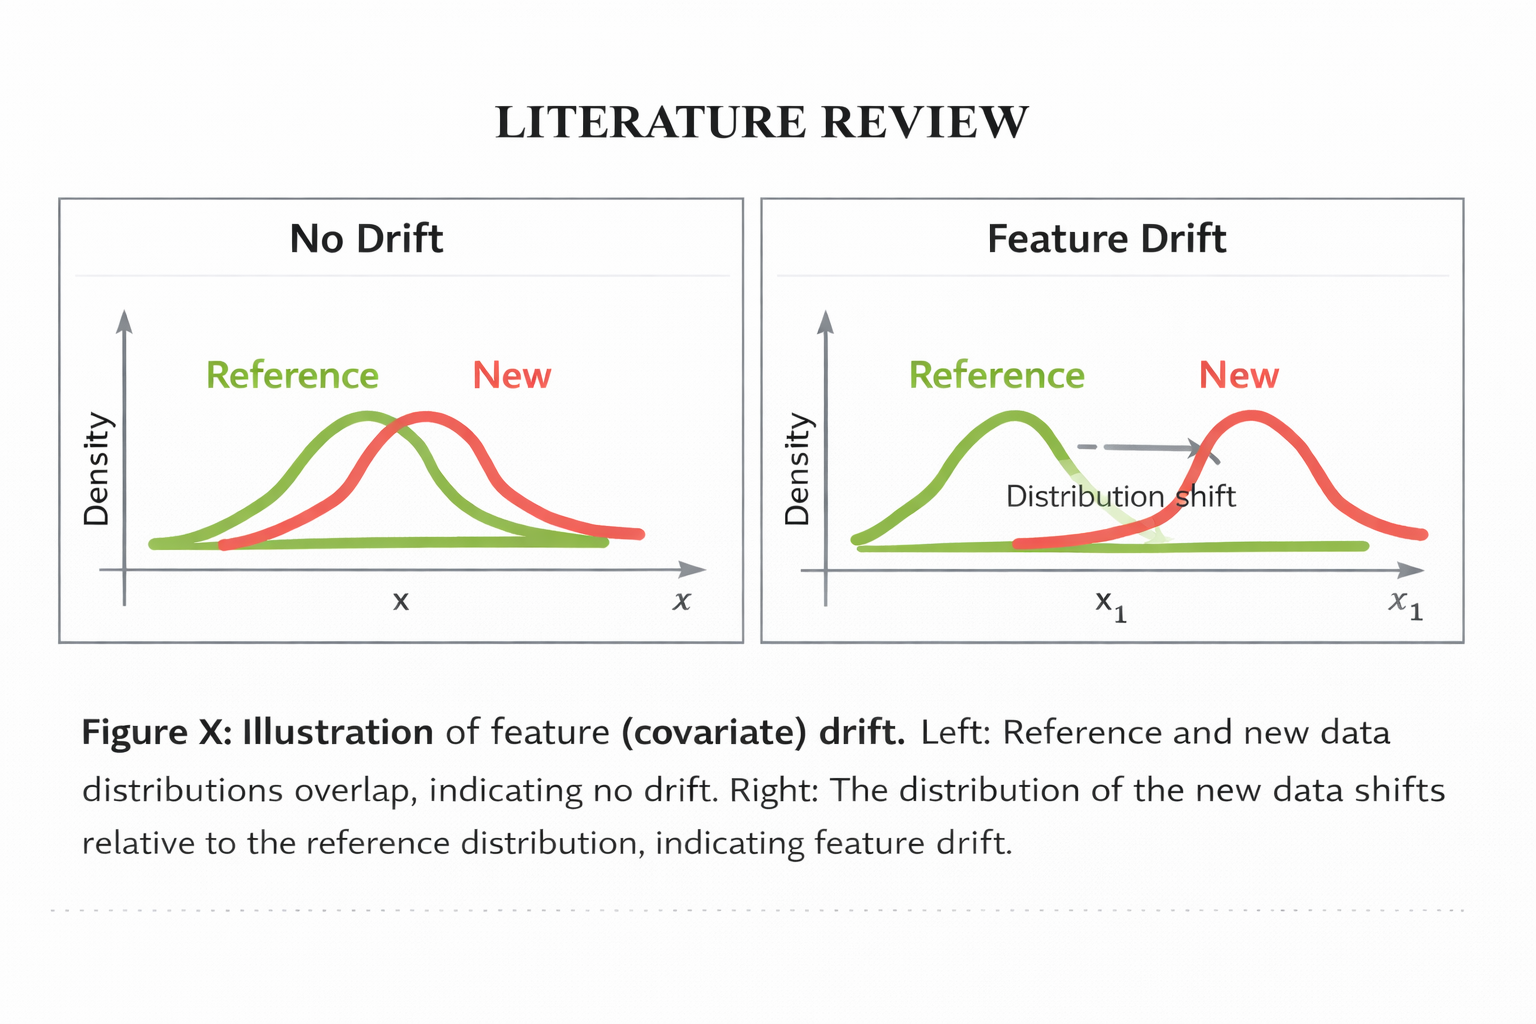
\includegraphics[width=.95\textwidth,keepaspectratio]{figures/figure-1.png}
    \caption[No drift versus drift for a discriminative classifier]{Comparison of no drift versus drift scenarios. Left: When distributions overlap, the discriminative classifier cannot distinguish data sources (AUC $\approx$ 0.5). Right: When drift occurs, distributions shift and the classifier can distinguish sources (AUC $\gg$ 0.5).}
    \label{fig:feature-drift}
\end{figure}

\section{Overview}
Drift detection addresses the challenge that arises when the statistical characteristics of data evolve over time in a manner that impacts the validity of a machine learning model \citep{Lu2018, Gama2014}. According to \citet{Bayram2022}, when users, environments, data sources, or the relationships between labels and features change, model accuracy can diminish. \citet{Gama2014} and \citet{Sculley2015} emphasise that drift detection identifies such modifications early, allowing practitioners to adapt, retrain, or update the model accordingly. A robust understanding of drift types and detection methods is essential for designing effective monitoring systems.

\section{Historical Evolution of Drift Detection}
The study of distribution drift has evolved from foundational statistical concepts to integrated AI governance over roughly seven decades. Table~\ref{tab:timeline} summarises the major eras.

\begin{table}[!htbp]
\centering
\caption{Historical evolution of drift detection research.}
\label{tab:timeline}
\begin{tabular}{p{3.5cm}p{10.5cm}}
\hline
\textbf{Era} & \textbf{Key Developments} \\
\hline
Early Foundations (1950s--1980s) & Statistical process control and sequential analysis laid the groundwork. \citet{Page1954} introduced the cumulative-sum (CUSUM) change-point test, which remains foundational for sequential change detection. Reservoir sampling \citep{Vitter1985} enabled representative subsampling of data streams. \\
\hline
Identification Era (1996--2004) & The term ``concept drift'' gained formal academic recognition \citep{WidmerKubat1996}. \citet{Gama2004} introduced the Drift Detection Method (DDM), using PAC-learning error-rate bounds to trigger alerts and establishing the supervised error-monitoring paradigm. \\
\hline
Windowing \& Statistical Tests (2007--2015) & \citet{BifetGavalda2007} proposed ADWIN (Adaptive Windowing), enabling drift detection without fixed window sizes by applying statistical tests over dynamically adjusted sub-windows. Non-parametric tests (KS, MMD) became standard for comparing reference and current distributions \citep{Rabanser2019, Gretton2012}. \\
\hline
Deep Learning \& High-Dimensionality (2018--2023) & As models moved to unstructured data, detection shifted toward monitoring internal latent representations \citep{Rabanser2019, Liu2020}. \citet{Gozuacik2019} introduced D3, demonstrating that discriminative classifiers could serve as powerful multivariate drift detectors. \citet{LopezPazOquab2017} formalised the classifier two-sample test (C2ST), providing theoretical backing for this approach. \\
\hline
Governance \& Attribution Era (2024--2026) & Drift detection became embedded in AI governance frameworks, and attention moved toward interpretable and statistically rigorous detection: TRIPODD \citep{TRIPODD2024} introduced feature-interaction hypothesis testing; E-C2ST \citep{EC2ST2024} enabled anytime-valid sequential testing via e-values; HDPD \citep{HDPD2024} decomposed performance gaps into $P(X)$ and $P(y|X)$ components with attributions. Cloud platforms added SHAP-based feature attribution monitoring \citep{TalySato2021, AWSSageMaker2025}. \citet{AdvAttackDrift2024} exposed vulnerabilities in discriminative detectors to adversarial evasion. \\
\hline
\end{tabular}
\end{table}

This progression, from reactive error monitoring to proactive analysis of feature distributions and attributions, provides the historical context for the present work.

\section{Types of Drift}
Drift can be categorised along two main dimensions: by the nature of the change (what component of the data-generating process is affected) and by the temporal pattern of the change (how the drift manifests over time) \citep{Lu2018, Gama2014}.

\subsection{Drift by Nature of Change}
Based on which component of the joint distribution $P(X, y)$ changes, the literature \citep{Lu2018, Gama2014, Tsymbal2004} classifies drift into the following types:

\textbf{Concept Drift (Real Drift):} The conditional distribution $P(y|X)$ changes over time while the feature distribution $P(X)$ may or may not change \citep{Lu2018, Zliobaite2010}. This represents a change in the underlying relationship between inputs and outputs: the ``concept'' the model has learned becomes invalid. For example, the factors that determine creditworthiness may evolve due to economic shifts, even if the applicant characteristics (features) remain similar \citep{Gama2014}. Concept drift directly degrades model performance because the learned decision boundaries no longer reflect the true input-output relationship \citep{Lu2018}.

\textbf{Covariate Drift (Feature Drift / Virtual Drift):} The marginal distribution of input features $P(X)$ changes over time while the conditional relationship $P(y|X)$ remains stable \citep{Tsymbal2004, Shimodaira2000}. The ground-truth concept does not change, but the model may encounter inputs outside its training distribution. For example, a fraud detection model trained on transaction patterns from one demographic may receive data from a different user population, even though the definition of fraud remains unchanged \citep{Tsymbal2004}. Covariate drift can degrade model performance because the model is exposed to feature regions where it may not generalise well \citep{Shimodaira2000}.

\textbf{Prior Probability Drift (Label Shift):} The marginal distribution of labels $P(y)$ changes over time while $P(X|y)$ remains stable \citep{Tsymbal2004}. This occurs when the prevalence of different classes changes, for instance a seasonal increase in a particular disease that alters the class balance in medical diagnosis. This is sometimes called class imbalance shift \citep{Lu2018}.

\textbf{Note on Terminology:} The literature uses varied terminology \citep{Lu2018}. The term ``concept drift'' is sometimes used as an umbrella term for any distribution change affecting model performance \citep{Gama2014}, while some reserve it specifically for changes in $P(y|X)$ \citep{Tsymbal2004}. This thesis focuses primarily on covariate (feature) drift detection, as it enables early warning without requiring labels.

\subsection{Drift by Temporal Pattern}
Based on how drift manifests over time, the literature \citep{Lu2018, Gama2014, Zliobaite2010} categorises drift as follows:

\begin{itemize}
    \item \textbf{Abrupt (Sudden) Drift:} A rapid, discrete change where the data distribution shifts quickly from one state to another within a short time period \citep{Gama2014}.

    \item \textbf{Gradual Drift:} A new distribution progressively replacing the old one over an extended duration, with samples from both distributions interleaved during the transition period \citep{Lu2018}.

    \item \textbf{Incremental Drift:} Small but continuous changes accumulating over time, eventually resulting in a significant distributional shift \citep{Zliobaite2010}.

    \item \textbf{Recurring (Seasonal) Drift:} Previously observed distributions reappearing periodically due to cyclical patterns, such as seasonal effects in retail or recurring user behaviour patterns \citep{Lu2018, Gama2014}.
\end{itemize}

Understanding drift patterns is important for detector design: abrupt drift requires rapid response, gradual drift requires sustained sensitivity, and recurring drift benefits from mechanisms that can recognise previously seen distributions \citep{Gama2014}.

Figure~\ref{fig:temporal-patterns} illustrates the four patterns with the synthetic streams used in the experiments of this thesis (Section~\ref{sec:datasets}).

\begin{figure}[!htbp]
    \centering
    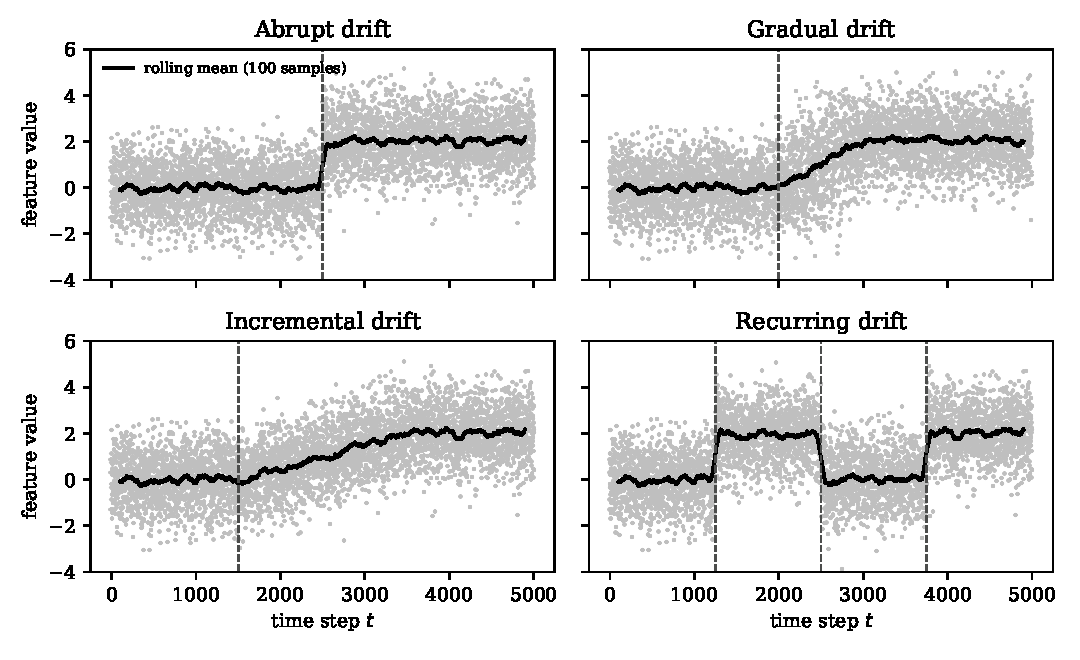
\includegraphics[width=0.95\textwidth]{figures/temporal_drift_patterns.pdf}
    \caption[Four temporal drift patterns]{The four temporal drift patterns in the synthetic streams of this thesis, shown for one feature. Grey points are individual samples, the black line is a rolling mean over 100 samples, and dashed lines mark the drift points.}
    \label{fig:temporal-patterns}
\end{figure}

\subsection{Summary Taxonomy}
Table~\ref{tab:drift-taxonomy} consolidates the drift classification used throughout this thesis.

\begin{table}[!htbp]
\centering
\caption{Taxonomy of drift types referenced in this thesis.}
\label{tab:drift-taxonomy}
\begin{tabular}{p{2.5cm}p{3cm}p{7.6cm}}
\hline
\textbf{Category} & \textbf{Type} & \textbf{Description} \\
\hline
\multirow{3}{*}{\parbox{2.5cm}{By Cause \\ \citep{Lu2018, Gama2014}}}
  & Data / Feature Drift & Change in the input distribution $P(X)$ without changing the relationship to the target. \\
  & Concept Drift & Change in the conditional $P(y \mid X)$, invalidating learned decision boundaries. \\
  & Prior Probability Drift & Change in the label distribution $P(y)$ while $P(X \mid y)$ is stable. \\
\hline
\multirow{4}{*}{\parbox{2.5cm}{By Pattern \\ \citep{Gama2014, Zliobaite2010}}}
  & Sudden (Abrupt) & Rapid, discrete shift between two distinct distributions. \\
  & Gradual & Old concept progressively replaced by a new one over an extended period. \\
  & Incremental & Small, continuous changes accumulating into a significant shift. \\
  & Recurring (Seasonal) & Previously observed distributions reappearing cyclically. \\
\hline
\end{tabular}
\end{table}

This thesis focuses primarily on \textbf{feature (covariate) drift}, that is, changes in $P(X)$, because it can be detected without ground-truth labels and provides early warning before model performance degrades.

\section{Classification of Drift Detection Methods}
Based on surveys of the drift detection literature \citep{Lu2018, Gama2014, Tsymbal2004, Hinder2024}, drift detection methods can be classified along several dimensions. According to \citet{Lu2018}, the most fundamental distinction is based on label availability: whether the method requires access to ground-truth labels (supervised) or operates without them (unsupervised).

\subsection{Supervised Drift Detection Methods}
Supervised detectors require ground-truth labels and monitor the error stream of the deployed model \citep{Gama2014, Gama2004}. They assume that a change in error behaviour, such as a higher error rate, errors that occur closer together, or a shift in the mean of a monitored loss, indicates drift \citep{Gama2004, BaenaGarcia2006}. The methods in this group differ mainly in the statistic they track and in the bound they use to decide that a change is significant. DDM compares the error rate and its standard deviation with thresholds derived from the binomial distribution \citep{Gama2004}. EDDM tracks the distance between consecutive errors, which makes it more sensitive to gradual drift \citep{BaenaGarcia2006}. The Page--Hinkley test accumulates the deviations of the monitored signal from its mean \citep{Page1954}, and HDDM-A and HDDM-W replace distributional assumptions with Hoeffding's inequality, using moving averages for abrupt change and weighted windows for gradual change \citep{FriasBlanco2015}.

Because these methods all watch the model's errors, they share the same strengths and weaknesses. Their alarms are tied directly to model performance, and their thresholds have a clear statistical meaning. However, they need labels, which are often delayed, expensive, or unavailable in production \citep{Lu2018, Sethi2017}. They also react only after drift has already degraded performance, and they cannot detect a change in $P(X)$ that has not yet affected the error rate.

\subsection{Unsupervised Drift Detection Methods}
Unsupervised drift detection methods do not require ground-truth labels and instead monitor changes in data distribution, model outputs, or internal representations \citep{Tsymbal2004, Hinder2024}. These methods enable earlier detection of distributional shifts, before performance degradation becomes observable, which makes them valuable in production environments with label delays \citep{Sethi2017}.

\subsubsection{Statistical Distribution-Based Methods}
Statistical methods compare a reference window with a current window through hypothesis tests or distance measures \citep{Rabanser2019, Raab2020, BifetGavalda2007}. They differ in what they compare. ADWIN compares the means of sub-windows of an adaptive window and shrinks the window when they differ, with guarantees on its false positive and false negative rates \citep{BifetGavalda2007}. KSWIN applies the Kolmogorov--Smirnov test to one feature at a time over sliding windows \citep{Raab2020}, and chi-squared tests play the same role for categorical or discretised features \citep{Lu2018}. Divergence measures such as the Kullback--Leibler divergence, the Jensen--Shannon divergence and the Hellinger distance quantify how far apart two estimated distributions are \citep{Dasu2006, DitzlerPolikar2011}, while the Maximum Mean Discrepancy (MMD) compares whole multivariate distributions through kernel embeddings \citep{Gretton2012}.

As a group, these methods are label-free, theoretically grounded and easy to interpret \citep{Rabanser2019}. Most of them, however, test one feature at a time. With $d$ features this requires $d$ tests, so unless the significance level is corrected, the probability of at least one false alarm grows with $d$, and changes in the joint distribution that leave every marginal unchanged are missed \citep{Lu2018, Webb2016}. Multivariate tests such as MMD avoid the per-feature problem, but their power depends on the choice of kernel \citep{Gretton2012}.

Table~\ref{tab:method-comparison} compares two widely used univariate methods, the Population Stability Index (PSI) and the KS test, with the multivariate discriminative approach used in this thesis.

\begin{table}[!htbp]
\centering
\caption{Comparison of drift detection approaches.}
\label{tab:method-comparison}
\begin{tabular}{p{2.5cm}p{3.6cm}p{3.6cm}p{3cm}}
\hline
\textbf{Method} & \textbf{Approach} & \textbf{Strengths} & \textbf{Limitations} \\
\hline
\textbf{PSI (Population Stability Index)} & Compares binned distributions of single features; PSI $> 0.25$ indicates significant drift & Simple, interpretable, industry standard & Univariate only; requires binning; misses feature correlations \\
\hline
\textbf{KS Test (Kolmogorov-Smirnov)} & Non-parametric test comparing cumulative distributions per feature & No distributional assumptions; exact p-values & Univariate only; multiple testing problem with many features \\
\hline
\textbf{Discriminative Classification} & Trains classifier to distinguish old vs. new data; uses AUC as drift signal & Multivariate; captures feature interactions; single unified test & Requires classifier training; no built-in feature attribution \\
\hline
\end{tabular}
\end{table}

Because PSI and the KS test are univariate, monitoring $d$ features requires $d$ separate tests. The discriminative approach instead tests the joint distribution of all $d$ features with a single classifier.

\subsubsection{Model-Based Discriminative Methods}
Discriminative methods train an auxiliary classifier to tell reference samples from current samples \citep{LopezPazOquab2017, Pan2020, Sethi2017}. If the classifier separates the two sets better than chance, the distributions differ. The methods in this group differ in what they read from the classifier. Domain classifiers, also called adversarial validation in industry practice, use the accuracy or AUC of a logistic regression, random forest, or gradient boosting model trained on the two windows \citep{Pan2020, Qian2021}. D3 applies this idea to data streams with a logistic regression classifier and a fixed AUC threshold \citep{Gozuacik2019}, and it is one of the three detectors recommended by a recent benchmark \citep{Lukats2024}. Margin density methods such as MD3 instead track the proportion of samples that fall close to the decision boundary of a classifier \citep{Sethi2017}.

The main strength of the group is that one classifier tests all features jointly and can capture non-linear changes that marginal tests miss \citep{LopezPazOquab2017}. No labels are needed, only the window that each sample came from \citep{Pan2020}. The costs are that a classifier must be trained at every monitoring step, that the results depend on the classifier and its hyperparameters, and that a raw AUC or margin value has no statistical calibration unless a test, such as a permutation test, is added \citep{Sethi2017, LopezPazOquab2017}.

\subsubsection{Representation-Based Methods}
Representation-based methods monitor learned representations rather than raw features \citep{Rabanser2019, Liu2020}. They compute distances such as the Wasserstein distance or MMD between reference and current embeddings taken from intermediate layers of a neural network \citep{Rabanser2019}, or they track the stability of learned representations using ideas from domain adaptation and transfer learning \citep{Long2016}. These methods suit deep learning systems in which raw feature distributions do not reflect semantically meaningful changes \citep{Liu2020}, but they require a representation model and are less relevant for the tabular streams studied in this thesis.

\subsubsection{Prediction-Based and Output-Based Methods}
Prediction-based methods monitor the outputs of the deployed model without checking whether they are correct \citep{Sethi2017, Gozuacik2019}. They track the distribution of predicted classes or scores \citep{Gozuacik2019}, or the entropy and confidence of the predictions, under the assumption that rising uncertainty indicates out-of-distribution inputs \citep{Guo2017}. Their weakness is calibration: modern models, deep networks in particular, are often poorly calibrated, and under distribution shift their confidence may not change in step with their errors \citep{Guo2017, Ovadia2019}. The prediction entropy signal used in EADD (Chapter~\ref{chap:methodology}) differs from these methods because it is computed from the discriminator that separates the two windows, not from the deployed model.

\subsubsection{Unsupervised Detectors Evaluated in Recent Benchmarks}
\citet{Lukats2024} reviewed ten fully unsupervised drift detectors and evaluated seven of them on eleven real-world data streams; the other three were too slow or depended too much on chance. They also found that the size of the observed samples was one of the most influential hyperparameters. The detectors they studied can be grouped by the mechanism they use.

The discriminative group is represented by D3 \citep{Gozuacik2019}, which achieved the best mean time ratio in the benchmark but, like the other detectors, reports only that drift occurred \citep{Lukats2024}.

Clustering-based detectors summarise each window with clusters and test whether the clusters change. CSDDM reduces dimensionality with PCA, clusters the data with K-Means, and applies statistical tests to the clusters \citep{CSDDM2021}, while UCDD assigns pseudo-labels from cluster membership and monitors shifts of the cluster boundary \citep{UCDD2020}. CSDDM was among the detectors that performed well on the benchmark's lift-per-drift metric, which measures how much classifier accuracy improves per detected drift \citep{Lukats2024}.

Density-based detectors model the reference distribution and flag new data that fit the model poorly. SPLL fits a semi-parametric density model and monitors the log-likelihood of new observations \citep{SPLL2013}, NN-DVI tracks changes in nearest-neighbour density \citep{NNDVI2018}, OCDD fits a one-class SVM to the reference data and counts the samples that fall outside its boundary \citep{OCDD2021}, and BNDM compares windows with a Bayesian non-parametric P\'{o}lya tree test. These detectors respond well to sudden changes in density, but they are sensitive to the size of the reference sample: BNDM signalled drift periodically when it observed few samples, and many OCDD configurations showed the same periodic behaviour \citep{Lukats2024}.

A last group reduces the stream to a simpler signal. IBDD converts windows of numerical data into images and compares the images \citep{IBDD2021}, and UDetect applies Shewhart control charts to the standard deviation of each window. IBDD achieved the best classifier accuracy in the benchmark because it can signal drift again immediately after a reset, but it was among the worst detectors on mean time ratio, and 45\% of the UDetect configurations detected no drift at all \citep{Lukats2024}.

Across these groups, the benchmarked detectors report whether drift occurred but not where it occurred \citep{Lukats2024}. D3 is the only discriminative detector in the benchmark, and it relies on a fixed AUC threshold rather than a calibrated test.

\subsection{Hybrid and Ensemble Methods}
Hybrid approaches combine several sources of information, such as model predictions, embeddings, operational signals and metadata, into a single context-weighted drift score, while ensemble approaches combine several base detectors through voting, weighting, or meta-learning to reduce both false alarms and missed detections \citep{Gama2014, Krawczyk2017}. These approaches can be more robust than any single detector, but they inherit the label or context requirements of their components, and misspecified context can cause missed detections or spurious alarms \citep{Krawczyk2017}.

\section{Limitations of Existing Methods}
Each group of methods has characteristic limitations. Supervised methods need timely labels and detect drift only after performance has degraded \citep{Lu2018, Sethi2017}. Statistical tests are sensitive to noise, mostly test marginal distributions, and raise more false alarms as the number of tested features grows \citep{Rabanser2019, Lu2018, Webb2016}. Prediction-based and uncertainty-based methods depend on model calibration, which is often poor under distribution shift \citep{Guo2017, Ovadia2019}, and context-aware methods depend on context variables that may be incomplete or may drift themselves \citep{Krawczyk2017}.

Discriminative tests avoid several of these problems. They test the joint feature distribution directly, need neither labels nor calibrated model outputs, and make no assumption about which features matter \citep{LopezPazOquab2017, Pan2020}. In streaming drift detection, however, they have mostly been used with fixed thresholds, as in D3 \citep{Gozuacik2019}.

\section{Drift Mitigation and Adaptation Strategies}
Detecting drift is only the first step; production systems must also respond to it. The literature describes five principal mitigation strategies, each with distinct trade-offs \citep{Lu2018, Gama2014, Krawczyk2017}:

\begin{enumerate}
    \item \textbf{Periodic Retraining:} The model is retrained on the latest data at fixed intervals (e.g., weekly or monthly) or triggered by drift alerts. This is the most common industrial approach because of its operational simplicity, but fixed schedules may retrain unnecessarily or react too slowly \citep{Gama2014}.

    \item \textbf{Weighted Retraining:} Old and new data are combined for retraining, but recent examples receive higher weights. This preserves long-term knowledge while prioritising current patterns, and is particularly effective for gradual drift \citep{Krawczyk2017}.

    \item \textbf{Ensemble Methods:} A library of models (for example, one per season or data regime) is maintained, and predictions are combined via voting, stacking, or dynamic weighting. When drift is detected, poorly performing members are discarded and new ones trained on the current distribution \citep{Krawczyk2017}.

    \item \textbf{Online / Incremental Learning:} The model is updated continuously as each new data point (or mini-batch) arrives, making it naturally adaptive to gradual and incremental drift. This is common in streaming applications such as fraud detection and recommendation systems \citep{Gama2014, Ditzler2015}.

    \item \textbf{Human-in-the-Loop:} Uncertain or drifted samples are routed to human experts for re-labelling, which feeds into the next training iteration. This strategy is essential in domains where errors carry high cost (e.g., healthcare, autonomous driving) and labelling is expensive \citep{Lu2018}.
\end{enumerate}

\section{Related Work: Discriminative and Attribution Approaches}

\subsection{Discriminative Distribution Testing}
Discriminative approaches to distribution comparison reframe the problem as a binary classification task: a classifier is trained to predict whether each instance originates from a reference distribution or a target distribution. High discriminative performance (AUC $\gg 0.5$) indicates the distributions are statistically separable; near-random performance suggests they are indistinguishable \citep{Pan2020, Qian2021}.

\citet{Pan2020} used this approach at Uber for the MaLTA user targeting system, training a classifier to detect mismatch between training and deployment data and retraining when the two were strongly separable. \citet{Qian2021} applied discriminative testing to manage dataset shift in credit scoring. D3 \citep{Gozuacik2019} turned the idea into a streaming detector that trains logistic regression classifiers on sliding windows and signals drift when the AUC exceeds a fixed threshold of 0.7. D3 achieved the best mean time ratio in the \citet{Lukats2024} benchmark. However, D3 applies no formal significance test; its fixed threshold is not calibrated, which can make it vulnerable to false alarms on autocorrelated data.

The \textit{classifier two-sample test} (C2ST), formalised by \citet{LopezPazOquab2017}, provided theoretical foundations for the discriminative approach: significance is calibrated via permutation testing, allowing principled Type~I error control. The approach is label-independent, model-agnostic, and makes no assumptions about which features are important. \citet{EC2ST2024} extended C2ST with anytime-valid e-values for sequential monitoring, and \citet{MCD2024} proposed Maximum Concept Discrepancy, which uses contrastive learning as an alternative to classifier-based testing for online drift detection. C2ST and E-C2ST were designed for distribution testing rather than for streaming drift detection, and neither provides feature-level attribution of the detected shift.

D3 and other C2ST-based streaming detectors usually discard the trained classifier after computing the AUC. Practitioners therefore learn whether drift occurred but receive no guidance on which features caused it, even though the classifier has learned which features separate the two windows.

\subsection{Drift Localisation}
Drift localisation asks where a drift occurs \citep{HinderLocalization2024}. The question can be posed for regions of the data space, that is, which samples are affected, or for features, that is, which input dimensions are affected. \citet{HinderLocalization2024} formalise localisation as finding the smallest region of the data space whose removal leaves no drift, and they survey the methods that address it. Most of these methods are built on local drift detection. Binning methods such as kdq-trees partition the data space and compare the samples in each cell \citep{Dasu2006}. Neighbourhood methods compare the local density around each sample, as in the local drift degree of \citet{Liu2017LDD}. Model-based methods train a probabilistic classifier to separate time periods and read the affected regions from its predictions \citep{HinderLocalization2024}.

Feature-level localisation has developed alongside this work. \citet{Kulinski2020} framed the question of which features have shifted as a set of conditional distribution tests, one per feature, and proposed parametric and non-parametric versions based on the score function of a density model. \citet{HinderFeature2024} gave formal definitions of feature-wise drift that allow detector-agnostic selection of drifting features. TRIPODD \citep{TRIPODD2024} tests pre-specified feature interactions with power guarantees, at a cost that grows quadratically with the number of features.

Localisation methods therefore already exist for samples, regions and features. They differ in what they require: a density model \citep{Kulinski2020}, pre-specified interactions \citep{TRIPODD2024}, or batch access to the data \citep{HinderFeature2024}. A further option, discussed next, is to explain the classifier that a discriminative test has already trained.

\subsection{Feature Attribution for Drift Detection}
Feature attribution methods explain the output of a model in terms of its input features. SHAP assigns each feature its Shapley value \citep{Shapley1953} in a cooperative game whose players are the features \citep{Lundberg2017}, and TreeSHAP computes these values exactly and in polynomial time for tree ensembles \citep{LundbergInteraction2020}. Attribution has been connected to drift in two main ways.

The first way explains a domain classifier. \citet{Maggio2021} trained a classifier to separate old data from new data and ranked the features by the mean absolute SHAP value of the classifier's output. In that study, the SHAP ranking identified the corrupted features more reliably than the classifier's impurity-based feature importance. This is the same classifier that a discriminative drift detector already trains, so the ranking adds feature-level localisation at little extra cost. Its limitations come from SHAP itself: the attributions describe the classifier rather than the data-generating process, and they are correlational rather than causal \citep{CausalDrift2025}.

The second way monitors the attributions of the deployed model. \citet{LundbergInteraction2020} monitored the SHAP values of a deployed model over time to find problems in its data pipeline. \citet{Mougan2025} defined explanation shift as a change in the distribution of a model's explanations between training data and new data, and showed that it can reveal shifts that change model behaviour, including changes in feature interactions that per-feature distribution tests miss. Commercial monitoring services follow the same idea: Google Vertex AI and Amazon SageMaker Clarify compare the feature attributions of production predictions with a baseline computed during training \citep{TalySato2021, AWSSageMaker2025}.

A related line of work attributes changes in model performance, rather than changes in the data distribution, to features or to parts of the data-generating process. \citet{Zhang2023Attribution} treated the distributions that make up the data-generating process as players in a cooperative game and attributed a model's performance change to them with Shapley values. HDPD decomposes a performance gap into covariate and conditional components with per-feature attributions \citep{HDPD2024}, DBShap separates virtual and real drift with distributional Shapley values \citep{DBShap2024}, and XPE combines optimal transport with Shapley values to explain how feature shifts affect performance \citep{XPE2024}. These methods require labels. A recent systematic review found that most work on explaining drift adapts static explanation methods to streaming data without addressing scalability or interactions between features \citep{XAIDriftSurvey2025}.

SHAP-based ranking of the features that separate two windows has therefore been used before \citep{Maggio2021}. This thesis does not claim it as a contribution; EADD uses it as one component of the framework.

\subsection{Other Recent Directions}
Other recent work has addressed label efficiency, explanation quality and robustness. Semi-supervised and student--teacher methods reduce or remove the need for labels \citep{CDSeer2024, STUDD2022}, per-label embedding monitoring extends drift detection to unstructured data \citep{DriftLens2024}, and autoregressive error monitoring adds confidence intervals to supervised detection \citep{ADDM2022}. For explanations, SGShift characterises concept shift with generalised additive models and controls the false discovery rate with knockoffs \citep{SGShift2025}, and \citet{CausalDrift2025} argue that drift explanations need causal rather than correlational attribution to guide remediation. \citet{AdvAttackDrift2024} showed that adversarially constructed data streams can evade common drift detectors, including discriminative ones.

\section{Gap in the Literature}
The review shows that the components of a discriminative drift detector that is both calibrated and interpretable already exist, but they have not been combined and evaluated together in a streaming setting. A classifier two-sample test can be calibrated with a permutation test \citep{LopezPazOquab2017}, but a fixed-budget permutation test retrains the classifier many times at every alarm, and D3, which a recent benchmark recommends, uses an uncalibrated fixed threshold instead \citep{Gozuacik2019, Lukats2024}. Sequential stopping rules that preserve the Type~I error of Monte Carlo tests \citep{Gandy2009} have not, to our knowledge, been applied to discriminative drift detection, and e-value tests \citep{EC2ST2024} were designed for distribution testing rather than for streaming detection.

A second gap concerns how discriminative detectors are compared. A new discriminative detector usually differs from D3 in its classifier, its window sizes, and the way it maintains its reference data. A comparison that changes all of these at once cannot show which of them causes the differences in detection delay, missed drifts and false alarms. Finally, feature-level localisation methods \citep{Kulinski2020, HinderFeature2024, TRIPODD2024} and SHAP explanations of domain classifiers \citep{Maggio2021, Mougan2025} answer the question of which features drifted, but they are usually run separately from, and after, detection.

This thesis addresses these gaps with EADD, an integrated framework that combines a LightGBM classifier two-sample test, a reservoir-sampled reference window, prediction entropy monitoring and an adaptive sequential permutation test, and that reports a TreeSHAP feature ranking for every confirmed drift. The evaluation includes an ablation that changes one design choice at a time.


\chapter{Research Methodology} \label{chap:methodology}

This chapter first states the research questions and hypotheses, then gives an overview of the methodology and describes each of its steps: the datasets, the EADD framework, the baseline detectors, the implementation and its validation, the evaluation metrics, and the experimental design with its statistical analysis.

\section{Research Questions}
\label{sec:rq}

Based on the gaps identified in Chapter~\ref{chap:literature}, this thesis investigates two research questions:

\begin{itemize}
    \item \textbf{RQ1 (Detection Accuracy):} Does EADD achieve comparable or better drift detection performance (detection delay and missed detections) than state-of-the-art unsupervised detectors on synthetic and real-world data streams?

    \item \textbf{RQ2 (Robustness):} Does EADD's permutation test reduce false alarm rates on stable data compared with threshold-based approaches such as D3?
\end{itemize}

\section{Hypotheses}
\label{sec:hypotheses}

Two formal hypotheses were tested:

\begin{itemize}
    \item \textbf{H1 (Detection Coverage):} EADD detects a broader range of temporal drift patterns than D3. H1a compares the drift streams that each detector detects (Experiments~1 and~4), and H1b compares detection delay on the streams that both EADD and D3 detect.

    \item \textbf{H2 (False Alarm Reduction):} EADD produces significantly fewer false alarms than D3 on stable data. Formally, $H_0$: $\text{FA}_{\text{EADD}} \geq \text{FA}_{\text{D3}}$ vs $H_1$: $\text{FA}_{\text{EADD}} < \text{FA}_{\text{D3}}$, where FA is the number of false alarms per stream. The hypothesis is tested with a one-sided Mann--Whitney U test ($\alpha = 0.05$) at several D3 thresholds ($\tau \in \{0.6, 0.7, 0.8\}$) in Experiment~3.
\end{itemize}

\section{Overview of the Methodology}
Figure~\ref{fig:research-methodology} summarises the methodology. First, synthetic, semi-synthetic and real-world data streams are collected (Section~\ref{sec:datasets}). Second, each stream is processed by EADD (Section~\ref{sec:eadd}) and by the baseline detectors (Section~\ref{sec:baselines}). The baselines include seven unsupervised detectors from the \citet{Lukats2024} benchmark and ablated versions of D3 and EADD that change one design choice at a time. Third, the detections are compared with the known drift points, or counted on stable streams that contain no drift, using the metrics in Section~\ref{sec:metrics}. Section~\ref{sec:design} describes the four experiments and the statistical tests.

\begin{figure}[!htpb]
    \centering
    \begin{tikzpicture}[
        node distance=0.6cm,
        stage/.style={rectangle, draw=black!65, fill=gray!10,
                      rounded corners=2pt, text width=12.5cm,
                      align=center, font=\small, inner xsep=8pt, inner ysep=6pt},
        arr/.style={-{Stealth[scale=0.85]}, semithick, black!70}
    ]
    \node[stage] (data) {%
        \textbf{1. Data Collection}\\[2pt]
        Synthetic drift streams (abrupt, gradual, incremental, recurring)\\
        Synthetic stable streams (i.i.d., AR(1), heteroscedastic, correlated)\\
        Semi-synthetic and real-world streams from \citet{Lukats2024}};
    \node[stage, below=of data] (detect) {%
        \textbf{2. Drift Detection}\\[2pt]
        EADD; D3 and D3-LightGBM; EADD without ASPT\\
        BNDM, CSDDM, IBDD, OCDD, SPLL and UDetect};
    \node[stage, below=of detect] (eval) {%
        \textbf{3. Evaluation}\\[2pt]
        MTD, missed detection rate, false alarms, precision, recall, runtime\\
        One-sided Mann--Whitney U test for false alarms};
    \draw[arr] (data) -- (detect);
    \draw[arr] (detect) -- (eval);
    \end{tikzpicture}
    \caption[Overview of the research methodology]{Overview of the research methodology: data collection, drift detection with EADD and the baseline detectors, and evaluation.}
    \label{fig:research-methodology}
\end{figure}

\section{Datasets}
\label{sec:datasets}
The population of interest is numerical data streams that are monitored for feature drift without labels. Following the benchmark of \citet{Lukats2024}, the experiments use a sample of synthetic streams with known drift points, semi-synthetic streams, and real-world streams.

\textbf{Synthetic Drift Streams:}
Each synthetic drift stream has $n = 5{,}000$ samples and $d = 5$ independent features. Before the drift, each feature follows $\mathcal{N}(0, 1)$; after the drift, its mean is shifted to $2$. The four streams differ in how the shift happens:
\begin{itemize}
    \item \textbf{Abrupt:} the mean shifts at $t = 2{,}500$.
    \item \textbf{Gradual:} between $t = 2{,}000$ and $t = 3{,}000$, each sample is drawn from the new distribution with a probability that rises linearly from 0 to 1.
    \item \textbf{Incremental:} the mean rises linearly from 0 to 2 between $t = 1{,}500$ and $t = 3{,}500$.
    \item \textbf{Recurring:} the stream alternates between the two distributions every 1{,}250 samples, giving drift points at $t = 1{,}250$, $2{,}500$ and $3{,}750$.
\end{itemize}

\textbf{Synthetic Stable Streams:}
Four stable streams with $n = 10{,}000$ samples, $d = 5$ features and no drift are used to measure false alarms:
\begin{itemize}
    \item \textbf{Gaussian i.i.d.:} independent samples from $\mathcal{N}(0, 1)$.
    \item \textbf{Autocorrelated AR(1):} $x_t = 0.7\, x_{t-1} + \epsilon_t$ with $\epsilon_t \sim \mathcal{N}(0, 1)$.
    \item \textbf{Heteroscedastic:} zero mean with a time-varying standard deviation
    \[ \sigma_t = 1 + 0.15 \sin(2\pi t / 2{,}000). \]
    \item \textbf{Correlated features:} multivariate normal with correlation $0.5^{|i-j|}$ between features $i$ and $j$.
\end{itemize}

\textbf{Semi-Synthetic Streams:}
SineClusters and WaveformDrift2 from the \citet{Lukats2024} framework have annotated drift points and are used in the supplementary multi-detector run of Experiment~2.

\textbf{Real-World Benchmark Datasets:}
Thirteen data streams were used for the primary real-world evaluation, drawn from the \citet{Lukats2024} benchmark suite and spanning diverse domains and drift characteristics. Four streams have annotated ground-truth drift points; nine are unannotated.

\textit{Annotated (known drift points):}
\begin{itemize}
    \item \textbf{INSECTS Abrupt Balanced} \citep{Souza2020}: 52,848 samples $\times$ 33 features; abrupt sensor drift in insect flight patterns (5 annotated drift points).
    \item \textbf{INSECTS Gradual Balanced} \citep{Souza2020}: 24,150 samples $\times$ 33 features; slow gradual sensor drift (1 annotated drift point).
    \item \textbf{INSECTS Incremental-Abrupt Balanced} \citep{Souza2020}: 79,986 samples $\times$ 33 features; incremental drift followed by abrupt reset (2 annotated drift points).
    \item \textbf{INSECTS Incremental-Reoccurring Balanced} \citep{Souza2020}: 79,986 samples $\times$ 33 features; incremental drift with reoccurring concept (2 annotated drift points).
\end{itemize}

\textit{Unannotated (no ground-truth drift labels):}
\begin{itemize}
    \item \textbf{Electricity (Elec2)} \citep{Harries1999}: 45,312 samples $\times$ 8 features; electricity pricing data with natural market fluctuations.
    \item \textbf{INSECTS Incremental Balanced} \citep{Souza2020}: 57,018 samples $\times$ 33 features.
    \item \textbf{Luxembourg} \citep{Lukats2024}: 1,900 samples $\times$ 31 features; financial data stream.
    \item \textbf{NOAA Weather} \citep{Lukats2024}: 18,159 samples $\times$ 8 features; weather measurements with temporal drift.
    \item \textbf{Outdoor Objects} \citep{Lukats2024}: 4,000 samples $\times$ 21 features; object recognition features with environmental variation.
    \item \textbf{Ozone} \citep{Lukats2024}: 2,534 samples $\times$ 72 features; atmospheric ozone level monitoring.
    \item \textbf{PokerHand} \citep{Lukats2024}: 829,201 samples $\times$ 10 features, of which the first 100,000 were used; card hand classification stream.
    \item \textbf{Powersupply} \citep{Lukats2024}: 29,928 samples $\times$ 2 features; power consumption data with usage pattern changes.
    \item \textbf{RialtoBridge Timelapse} \citep{Lukats2024}: 82,250 samples $\times$ 27 features; visual feature stream from a bridge camera.
\end{itemize}

All datasets were processed in streaming fashion, with features used for drift detection. For datasets with known drift points (e.g., INSECTS variants with drift indices at specific sample positions), ground truth was used for computing detection metrics. The INSECTS datasets were particularly valuable as they provide exact drift timestamps, enabling precise measurement of detection delay and false alarm rates.

\section{The EADD Framework}
\label{sec:eadd}
EADD treats feature drift ($P(X)$ shift) detection as binary classification: if a classifier can reliably distinguish reference data from current data based solely on features, the distributions have diverged \citep{LopezPazOquab2017, Gozuacik2019}. D3 \citep{Gozuacik2019} uses this principle with a fixed AUC threshold, and \citet{LopezPazOquab2017} showed how to calibrate the test with permutations. EADD combines these ideas with a long-memory reference window, a sequential version of the permutation test, and a feature ranking for each confirmed drift.

\subsection{Problem Formulation}
\label{sec:problem}
Let $\{x_t\}_{t=1}^{T}$, with $x_t \in \mathbb{R}^d$, denote a stream of feature vectors. At each monitoring point $t$, a detector compares two windows:
\begin{itemize}
    \item a reference window $W_{ref}$ of $N_{ref}$ samples, assumed to represent the baseline feature distribution $P_{ref}(X)$, and
    \item a current window $W_{cur}$ containing the $N_{cur}$ most recent samples, drawn from the current distribution $P_{cur}(X)$.
\end{itemize}
Feature drift at time $t$ means $P_{cur}(X) \neq P_{ref}(X)$. The detector therefore tests
\begin{equation}
H_0: P_{ref}(X) = P_{cur}(X) \quad \text{versus} \quad H_1: P_{ref}(X) \neq P_{cur}(X)
\label{eq:drift-test}
\end{equation}
and outputs a decision $d_t \in \{0, 1\}$, where $d_t = 1$ signals drift. In EADD, the test statistic is the cross-validated AUC of a classifier $f_\theta$ trained to separate $W_{ref}$ from $W_{cur}$. The symbol $\tau$ denotes the AUC screening threshold, $\alpha$ the significance level, and $B_{\min}$ and $B_{\max}$ the minimum and maximum numbers of permutations used by the permutation test.

Figure~\ref{fig:methodology-detailed-architecture} shows the steps of EADD, and Table~\ref{tab:eadd-alignment} lists the methods each step builds on.

\begin{figure}[!htpb]
    \centering
    \begin{tikzpicture}[
        node distance=0.56cm,
        proc/.style={rectangle, draw=black!65, fill=gray!10,
                     rounded corners=2pt, text width=7.8cm, minimum height=0.95cm,
                     align=center, font=\small, inner xsep=6pt, inner ysep=5pt},
        term/.style={rectangle, draw=black!55, fill=white,
                     rounded corners=2pt, text width=7.8cm,
                     align=center, font=\small, inner xsep=7pt, inner ysep=5pt},
        dec/.style={diamond, draw=black!65, fill=white,
                    aspect=2.2, align=center, font=\small, inner sep=2pt},
        arr/.style={-{Stealth[scale=0.85]}, semithick, black!70},
        lbl/.style={font=\footnotesize, fill=white, inner sep=1pt, text=black!70}
    ]

    \node[term] (input) {\textbf{Input Data Stream} \quad $\{x_t\}_{t=1}^{T}$};

    \node[proc, below=of input] (s1) {%
        \textbf{Step 1. Adaptive Reference Windowing}\\[-1pt]
        {\footnotesize Reservoir sampling for $W_\mathrm{ref}$\,; sliding window for $W_\mathrm{cur}$}
    };

    \node[proc, below=of s1] (s2) {%
        \textbf{Step 2. Discriminative Classification (C2ST)}\\[-1pt]
        {\footnotesize LightGBM on $W_\mathrm{ref} \cup W_\mathrm{cur}$\,; monitor AUC and $H_\mathrm{pred}$}
    };

    \node[dec, below=0.72cm of s2] (dec1) {$\mathrm{AUC} > \tau$?};

    \node[proc, below=0.72cm of dec1] (s3) {%
        \textbf{Step 3. Statistical Significance Testing (ASPT)}\\[-1pt]
        {\footnotesize Adaptive sequential permutation test with early stopping}
    };

    \node[dec, below=0.72cm of s3] (dec2) {$p < \alpha$?};

    \node[proc, below=0.72cm of dec2] (s4) {%
        \textbf{Step 4. Feature Ranking}\\[-1pt]
        {\footnotesize TreeSHAP ranking of the features that separate the two windows}
    };

    \node[term, below=of s4] (output) {%
        \textbf{Drift Alert Output}\\[-1pt]
        {\footnotesize uncertainty ($H_\mathrm{pred}$), significance ($p$), ranked features (SHAP)}
    };

    \draw[arr] (input) -- (s1);
    \draw[arr] (s1) -- (s2);
    \draw[arr] (s2) -- (dec1);
    \draw[arr] (dec1.south) -- node[lbl, right=2pt] {Yes} (s3.north);

    \draw[arr] (s3) -- (dec2);
    \draw[arr] (dec2.south) -- node[lbl, right=2pt] {Yes} (s4.north);

    \draw[arr] (s4) -- (output);

    \end{tikzpicture}
    \caption[Architecture of EADD]{Architecture of EADD: adaptive reference windowing, discriminative classification, ASPT significance testing, and TreeSHAP feature ranking for each confirmed drift.}
    \label{fig:methodology-detailed-architecture}
\end{figure}

\begin{table}[!htbp]
\centering
\caption{EADD components and the methods they build on.}
\label{tab:eadd-alignment}
\begin{tabular}{p{3.6cm}p{5cm}p{5cm}}
\hline
\textbf{Component} & \textbf{EADD Step} & \textbf{Based On} \\
\hline
Reference memory & Step 1: reservoir-sampled $W_{ref}$ & Reservoir sampling \citep{Vitter1985} \\
Drift statistic & Step 2: cross-validated AUC of a LightGBM classifier & C2ST \citep{LopezPazOquab2017}; D3 \citep{Gozuacik2019}; LightGBM \citep{Ke2017} \\
Uncertainty signal & Step 2b: prediction entropy $H_{\text{pred}}$ & Shannon entropy \citep{Shannon1948} \\
Statistical confirmation & Step 3: adaptive sequential permutation test & Sequential Monte Carlo tests \citep{Gandy2009} \\
Feature ranking & Step 4: TreeSHAP ranking & SHAP \citep{Lundberg2017, LundbergInteraction2020}; \citet{Maggio2021} \\
\hline
\end{tabular}
\end{table}

\subsection{Step 1: Adaptive Reference Windowing}
To detect feature drift, the current data must be compared against a stable baseline. EADD maintains two windows consistent with established methodologies \citep{BifetGavalda2007, Tsymbal2004}:

\textbf{Reference Window ($W_{ref}$):} A buffer containing $N_{ref}$ historical samples representing the stable feature distribution $P_{ref}(X)$. Unlike sliding windows, which forget older data quickly, EADD uses \textbf{reservoir sampling} \citep{Vitter1985} so that the reference represents all samples seen since the last confirmed drift, not just the most recent batches.

\textbf{Current Window ($W_{cur}$):} A buffer containing the $N_{cur}$ most recent observations representing the current feature distribution $P_{cur}(X)$. As new data arrives, older samples are discarded to maintain responsiveness to recent changes.

\textbf{Update Mechanism:} At each monitoring step:
\begin{itemize}
    \item New samples enter $W_{cur}$
    \item Oldest samples exit $W_{cur}$
    \item Reservoir sampling maintains representative $W_{ref}$
    \item Upon confirmed drift, $W_{ref}$ is reset to the current window
\end{itemize}

According to \citet{Lu2018}, window sizes represent a bias-variance tradeoff: larger windows provide more stable estimates but slower response; smaller windows enable faster detection but higher variance.

\subsection{Step 2: Discriminative Classification}
This step implements the \textbf{classifier two-sample test} (C2ST) \citep{LopezPazOquab2017}, also referred to as ``discriminative classification'' or ``adversarial validation'' in industry practice \citep{Pan2020}, which forms the foundation of both D3 \citep{Gozuacik2019} and EADD. The question it asks is whether a model can tell the difference between old and new data.

\textbf{Construct Binary Classification Dataset:}
\begin{itemize}
    \item Label all samples from $W_{ref}$ as class 0 (``old'' / reference)
    \item Label all samples from $W_{cur}$ as class 1 (``new'' / current)
    \item Combined dataset: $X = W_{ref} \cup W_{cur}$, $y = \{0\}^{N_{ref}} \cup \{1\}^{N_{cur}}$
\end{itemize}

\textbf{Train Discriminative Classifier:}
A binary classifier $f_\theta$ is trained to predict the data source from the features alone. EADD uses \textbf{LightGBM} \citep{Ke2017}, a gradient boosting decision tree ensemble, as the default classifier. D3 \citep{Gozuacik2019} uses logistic regression, which can only separate the windows with a linear boundary; LightGBM can also capture non-linear differences and feature interactions. Experiment~4 measures how much this choice matters on its own.

\textbf{Measure Discriminative Performance:}
Classifier performance is evaluated with stratified 5-fold cross-validation:
\begin{itemize}
    \item \textbf{AUC-ROC:} the primary metric, the area under the ROC curve
    \item AUC $\approx$ 0.5: the classifier cannot distinguish $W_{ref}$ from $W_{cur}$ $\rightarrow$ \textbf{no feature drift}
    \item AUC $\gg$ 0.5: the classifier separates the windows $\rightarrow$ $P_{ref}(X) \neq P_{cur}(X)$ $\rightarrow$ \textbf{feature drift suspected}
\end{itemize}

If the AUC exceeds the screening threshold $\tau$, the alarm is passed to the significance test in Step~3. The term ``adversarial'' in EADD's name refers to this C2ST setting, in which a classifier is trained to distinguish two data sources, and not to adversarial attacks in the security or robustness sense.

\subsection{Step 2b: Prediction Entropy Monitoring ($H_{\text{pred}}$)}
After training the discriminative classifier (Step~2), EADD computes the \textbf{prediction entropy} $H_{\text{pred}}$ as an early-warning signal for distributional instability. This is the binary Shannon entropy \citep{Shannon1948} of the C2ST discriminator's output probabilities, averaged over all samples:

\begin{equation}
H_{\text{pred}} = \frac{-1}{n} \sum_{i=1}^{n} \left[\hat{p}_i \ln \hat{p}_i + (1 - \hat{p}_i) \ln (1 - \hat{p}_i)\right]
\label{eq:hpred}
\end{equation}

where $\hat{p}_i = f_\theta(x_i)$ is the discriminative classifier's predicted probability that sample $i$ belongs to the current window ($W_{cur}$), and $n = |W_{ref}| + |W_{cur}|$ is the combined sample count.

\textbf{Interpretation:}
\begin{itemize}
    \item $H_{\text{pred}} \approx \ln 2$: Maximum entropy; the classifier cannot distinguish windows $\rightarrow$ no distributional difference
    \item $H_{\text{pred}} \rightarrow 0$: Low entropy; the classifier clearly separates windows $\rightarrow$ strong drift signal
    \item Intermediate $H_{\text{pred}}$: Subtle distributional change that may not yet reach statistical significance
\end{itemize}

\textbf{Monitoring Property:}
$H_{\text{pred}}$ is computed at every monitoring step, including steps where the AUC has not yet reached $\tau$, so it gives a continuous view of how confidently the discriminator separates the two windows. It was intended as an early-warning signal for gradual and incremental drift. In the logs of the real-world experiments, however, $H_{\text{pred}}$ fell together with the AUC rather than ahead of it (Section~\ref{sec:component-analysis}), so this thesis does not claim an early-warning effect. A quantitative evaluation, including threshold selection and the precision and recall of pre-alarm warnings, is left to future work.

\textbf{Relationship to AUC:}
$H_{\text{pred}}$ and AUC are complementary signals. AUC measures overall discriminability, while $H_{\text{pred}}$ measures the confidence distribution of individual predictions. A high AUC with low entropy indicates clear, systematic drift; a moderately elevated AUC with higher entropy may indicate localised or emerging drift affecting only a subset of samples.

\subsection{Step 3: Adaptive Sequential Permutation Test (ASPT)}
A raw AUC score (e.g., 0.65) is inconclusive, as it may reflect genuine distributional change or statistical noise. D3 \citep{Gozuacik2019} relies on a fixed threshold (AUC $> 0.7$) without a significance test. \citet{LopezPazOquab2017} proposed the classifier two-sample test (C2ST) with significance testing, typically implemented as a fixed-budget permutation test \citep{Good2005} with a predetermined number $B$ of permutations.

\textbf{The Computational Problem:} A fixed-budget permutation test (e.g., $B=50$) wastes computation when the evidence is clear. If the actual AUC is 0.95, the first few permutations already establish significance and the remaining permutations add cost without information. Conversely, if the AUC is 0.52, early permutations quickly reveal non-significance.

\textbf{Adaptive Sequential Permutation Testing:}
EADD uses an \textbf{adaptive sequential permutation test} based on the sequential Monte Carlo framework of \citet{Gandy2009}. Instead of committing to a fixed budget $B$, ASPT monitors evidence accumulation after each permutation and terminates early when the decision boundary is crossed:

\begin{enumerate}
    \item \textbf{Initialise:} Set maximum budget $B_{\max}$, nominal significance level $\alpha$, and minimum sequential budget $B_{\min}$.
    \item \textbf{Sequential Execution:} For each permutation $i = 1, \ldots, B_{\max}$:
    \begin{itemize}
        \item Shuffle labels, retrain the discriminative classifier, compute $\text{AUC}^{(i)}_{\text{perm}}$
        \item Update running count: $c_i = \#\{j \leq i : \text{AUC}^{(j)}_{\text{perm}} \geq \text{AUC}_{\text{actual}}\}$
        \item \textbf{Early reject $H_0$ (confirm drift):} If $c_i = 0$ and $i \geq B_{\min}$ and the conservative bound $1/(i+1) < \alpha$ holds, terminate and confirm drift with $p = 1/(i+1)$.
        \item \textbf{Early accept $H_0$ (no drift):} If $c_i / i > 2\alpha$ and $i \geq B_{\min}$, the running exceedance rate far exceeds the nominal level; terminate and declare no drift with $p = (c_i + 1)/(i + 1)$.
    \end{itemize}
    \item \textbf{Terminal decision:} If $B_{\max}$ is reached, compute the standard empirical p-value: $p = (c_{B_{\max}} + 1) / (B_{\max} + 1)$. Drift is confirmed if $p < \alpha$.
\end{enumerate}

\textbf{Statistical Validity Note:} ASPT preserves the standard permutation p-value at termination, either by the full-budget estimate $p = (c_B + 1)/(B+1)$ or by the conservative early-reject upper bound $p = 1/(i+1)$ when no exceedances are observed. This keeps the stopping rule aligned with the permutation-test interpretation.

\textbf{Computational Savings:} ASPT logs the number of permutations executed per invocation. With $\alpha = 0.05$ and $B_{\min} = 10$, the earliest possible confirmation is at $i = 20$, where $1/21 \approx 0.048 < \alpha$, so a clear drift costs 20 permutations instead of $B_{\max} = 199$. Clear non-drift cases can stop after $B_{\min} = 10$ permutations, and only cases close to the decision boundary use the full budget.

\textbf{Interaction with the AUC Threshold:} ASPT runs only when the AUC exceeds the screening threshold $\tau$. Under the null hypothesis, the AUC of a classifier trained on shuffled labels stays close to 0.5, and with $N_{ref} = 500$ and $N_{cur} = 200$ it rarely moves far from that value. An observed AUC above $\tau = 0.7$ is therefore far into the tail of the permutation distribution, and ASPT is expected to confirm almost every alarm that reaches it. ASPT affects the decision mainly when $\tau$ is set closer to 0.5, which Experiment~4 examines.

\subsection{Step 4: Feature Ranking via TreeSHAP}
Once ASPT confirms drift ($p < \alpha$), EADD reports which features drive the separation between the two windows. D3 \citep{Gozuacik2019} discards the trained classifier after computing the AUC, although the classifier has learned which features differentiate the reference data from the current data. Following \citet{Maggio2021}, EADD explains the discriminative classifier with SHAP.

EADD applies \textbf{TreeSHAP} \citep{Lundberg2017, LundbergInteraction2020} to a LightGBM classifier trained on $W_{ref} \cup W_{cur}$. TreeSHAP computes exact Shapley values \citep{Shapley1953} in polynomial time for tree-based models. The per-feature ranking is computed as follows:
\begin{enumerate}
    \item Compute SHAP values using TreeSHAP
    \item Calculate the mean absolute SHAP value per feature: $\text{Importance}_i = \frac{1}{n} \sum_{j=1}^{n} |\text{SHAP}_{ij}|$
    \item Normalise to a contribution vector: $s_i = \frac{\text{Importance}_i}{\sum_k \text{Importance}_k}$, so that $\mathbf{s} = (s_1, \ldots, s_d)$ sums to 1
    \item Rank the features by $s_i$
\end{enumerate}

EADD also computes TreeSHAP interaction values \citep{LundbergInteraction2020} on a sample of 100 points and reports their mean absolute values for each feature pair. The ranking and the interaction values are provided as diagnostic output; their accuracy is not evaluated in this thesis.

\subsection{Model Adaptation Strategies}
According to \citet{Gama2014}, upon drift detection, the primary prediction model can be adapted:

\textbf{Strategy 1: Drift-Triggered Retraining}
\begin{itemize}
    \item Model is trained at initialisation
    \item Retraining occurs only when drift alarm is raised
    \item Reference window resets to current data after retraining
    \item According to \citet{Pan2020}, advantage: Conserves resources; exploits early detection for timely updates
\end{itemize}

\textbf{Strategy 2: Periodic Retraining (Baseline)}
\begin{itemize}
    \item Model is retrained at fixed intervals regardless of drift signals
    \item Advantage: Simple; does not depend on detector reliability
    \item According to \citet{Gama2014}, disadvantage: May retrain unnecessarily or too late
\end{itemize}

\textbf{Strategy 3: Continuous Update with Drift Weighting}
\begin{itemize}
    \item Online learning with sample weighting based on drift score
    \item According to \citet{Krawczyk2017}, recent samples receive higher weights when drift is detected
\end{itemize}

\section{Baseline Drift Detectors}
\label{sec:baselines}
EADD was benchmarked against seven state-of-the-art unsupervised drift detectors evaluated in the \citet{Lukats2024} survey, all of which operate without ground-truth labels:

\begin{itemize}
    \item \textbf{D3 (Discriminative Drift Detector)} \citep{Gozuacik2019}: Trains a logistic regression classifier to distinguish old from new data windows, using AUC as the drift signal. One of the three detectors recommended by the \citet{Lukats2024} benchmark.
    \item \textbf{BNDM (Bayesian Non-parametric Drift Monitor):} Uses a P\'{o}lya tree test to detect distributional changes without parametric assumptions.
    \item \textbf{CSDDM (Clustered Statistical Drift Detection Method)} \citep{CSDDM2021}: Applies PCA dimensionality reduction followed by K-Means clustering, then uses statistical tests to detect cluster shifts.
    \item \textbf{IBDD (Image-Based Drift Detector)} \citep{IBDD2021}: Converts numerical data streams into images and applies image comparison techniques to detect distributional changes.
    \item \textbf{OCDD (One-Class Drift Detector)} \citep{OCDD2021}: Uses one-class SVMs to define ``normal'' data boundaries and flags drift when incoming data falls outside these boundaries.
    \item \textbf{SPLL (Semi-Parametric Log-Likelihood)} \citep{SPLL2013}: Fits probability density models to reference data and detects drift when new observations have anomalously low likelihood.
    \item \textbf{UDetect (Univariate Detection):} Monitors standard deviation changes using Shewhart control charts.
\end{itemize}

Existing benchmark results for these seven detectors from the \citet{Lukats2024} framework were used for direct comparison with EADD's detection performance across the same datasets.

\textbf{Ablation Variants:}
EADD differs from D3 in its classifier, its window sizes, its reference memory, and its permutation test. To measure the effect of each difference, Experiment~4 adds the following variants, each of which changes one design choice:
\begin{itemize}
    \item \textbf{D3-LightGBM:} D3 with its logistic regression replaced by LightGBM with the same hyperparameters as EADD. Windows, 2-fold cross-validation and the fixed AUC threshold are unchanged.
    \item \textbf{D3-LightGBM (matched windows):} D3-LightGBM with EADD's window sizes ($N_{ref} = 500$, $N_{cur} = 200$).
    \item \textbf{EADD-NoASPT:} EADD without the permutation test; every alarm with $\text{AUC} > \tau$ is accepted.
    \item \textbf{EADD-NoASPT (fixed reference):} EADD-NoASPT in which $W_{ref}$ keeps the first $N_{ref}$ samples after the last confirmed drift instead of being updated by reservoir sampling.
    \item \textbf{Lower thresholds:} EADD and EADD-NoASPT with $\tau \in \{0.5, 0.6\}$ in addition to the default $\tau = 0.7$, so that ASPT, rather than the threshold, decides most alarms.
\end{itemize}

\section{Implementation and Validation}
\label{sec:implementation}
All detectors were run in Python. The seven baseline detectors and the dataset loaders come from the open-source implementation of the \citet{Lukats2024} benchmark, whose authors only included algorithms that could be implemented faithfully from their original descriptions; their unit tests were kept. EADD (\texttt{detectors/eadd.py}) and D3-LightGBM (\texttt{detectors/d3\_lightgbm.py}) were added to this code base and use LightGBM \citep{Ke2017} and scikit-learn. Unit tests check that ASPT confirms a clear shift after exactly 20 permutations with $p = 1/21$, that it stops early without a shift, that EADD raises no alarm on a stable stream and detects an abrupt shift after its onset, and that D3-LightGBM detects a simple shift once. All experiments use fixed random seeds, and the code, scripts and result files are available in the project repository\footnote{\url{https://github.com/NusratBegum/unsupervised-concept-drift-detection}}.

\section{Evaluation Metrics}
\label{sec:metrics}

Following \citet{Lu2018}, \citet{Lukats2024}, and \citet{Souza2020}, the following metrics were used to evaluate drift detection performance:

\begin{itemize}
    \item \textbf{Mean Time to Detection (MTD):} Average number of samples between a true drift point and the first detection within a tolerance window after it. Lower is better.
    \item \textbf{Missed Detection Rate (MDR):} Proportion of true drifts that were not detected within the tolerance window. Lower is better.
    \item \textbf{False Alarms (FA):} Number of detections that are not matched to a true drift point. On stable streams, every detection is a false alarm. Lower is better.
    \item \textbf{Precision and Recall:} On annotated real-world streams, the proportion of detections that match a known drift point and the proportion of known drift points that are detected. A detection matches a drift point if it occurs within 500 samples after it.
    \item \textbf{Detection Count:} On unannotated real-world streams, the number of detections, used as an indicator of selectivity.
    \item \textbf{Runtime:} Wall-clock time to process a stream.
\end{itemize}

\section{Experimental Design}
\label{sec:design}

Four experiments were designed to answer the research questions:

\textbf{Experiment 1: Multi-Detector Sensitivity to Temporal Drift Patterns}

Compared all eight detectors (EADD, D3, BNDM, CSDDM, IBDD, OCDD, SPLL, UDetect) on the four synthetic drift streams ($n = 5{,}000$), using the default configurations from the \citet{Lukats2024} framework. This experiment addresses RQ1 and H1.

\textbf{Experiment 2: Real-World Benchmark Comparison}

Benchmarked EADD against D3 across 13 real-world benchmark data streams (4 annotated + 9 unannotated) with three seeds, measuring precision, recall, MTD and detection counts. A supplementary multi-detector comparison (EADD, D3, BNDM, CSDDM, IBDD, OCDD, SPLL, UDetect) was also conducted on the first 20{,}000 samples of an 11-stream subset to place EADD within the full \citet{Lukats2024} benchmark field. This experiment addresses RQ1.

\textbf{Experiment 3: Robustness to Stable Data (False Alarm Evaluation)}

Counted false alarms on the four stable synthetic streams with zero actual drift (Gaussian i.i.d., autocorrelated, heteroscedastic, correlated features) over five runs, and compared EADD with D3 at AUC thresholds $\tau \in \{0.6, 0.7, 0.8\}$. This experiment addresses RQ2 and H2.

\textbf{Experiment 4: Component Ablation with a LightGBM D3}

Ran D3, the ablation variants of Section~\ref{sec:baselines}, and EADD on the synthetic drift streams of Experiment~1 (five seeds), on the stable streams of Experiment~3 (five runs), and on the 13 real-world streams of Experiment~2 (three seeds). Changing one design choice at a time shows whether EADD's results come from the classifier, the window sizes, the reference memory, the AUC threshold, or the permutation test. This experiment addresses RQ1 and RQ2.

\subsection{Statistical Analysis}
Results over several seeds or runs are summarised by their mean, and by their range where it matters for interpretation. H1a is tested with an exact one-sided sign test on the 20 synthetic drift streams of Experiment~4 (four drift types and five seeds): each stream counts for EADD if only EADD detects its drift and for D3 if only D3 does. H1b is tested with a two-sided Wilcoxon signed-rank test on the detection delays of the streams that both detectors detect. H2 is tested with a one-sided Mann--Whitney U test on the mean number of false alarms per stable stream type. Because only four stream types are compared, the exact p-value of this test is reported together with the normal approximation. All tests use $\alpha = 0.05$.

\section{Practical Considerations}

\textbf{Class Imbalance:} When $|W_{ref}| \neq |W_{cur}|$, use:
\begin{itemize}
    \item Stratified cross-validation
    \item Class-weighted classifiers
    \item According to \citet{LopezPazOquab2017}, AUC-ROC rather than accuracy
\end{itemize}

\textbf{Computational Efficiency:}
\begin{itemize}
    \item Use efficient classifiers (logistic regression, small random forests)
    \item Consider approximate methods for large windows
    \item According to \citet{Pan2020}, implement incremental training where possible
\end{itemize}

\textbf{Temporal Leakage Prevention:}
\begin{itemize}
    \item Use purged cross-validation to avoid temporal overlap between folds
    \item According to \citet{Souza2020}, ensure strict temporal ordering in train/test splits
\end{itemize}

\textbf{Threshold Calibration:}
\begin{itemize}
    \item Use validation data with known drift to tune $\tau$
    \item According to \citet{Pan2020}, consider adaptive thresholds based on baseline variance
\end{itemize}


\chapter{Results} \label{chap:results}

This chapter presents the results of the four experiments described in Section~\ref{sec:design}: sensitivity to temporal drift patterns, the real-world benchmark, false alarms on stable data, and the component ablation. The research questions and hypotheses are stated in Sections~\ref{sec:rq} and~\ref{sec:hypotheses}.

\section{Experimental Setup}

\textbf{Environment:} Experiments 1 and 3 were run in Python 3.10. Experiments 2 and 4 were run with Python 3.13, LightGBM 4.6 and scikit-learn 1.8 on the same code base (Section~\ref{sec:implementation}).

\textbf{EADD Configuration:}
\begin{itemize}
    \item \textbf{Reference Window ($N_{ref}$):} 500 samples
    \item \textbf{Current Window ($N_{cur}$):} 200 samples
    \item \textbf{AUC Threshold ($\tau$):} 0.7, as in D3 \citep{Gozuacik2019}
    \item \textbf{ASPT:} $B_{\max} = 199$ permutations, $B_{\min} = 10$, $\alpha = 0.05$ (adaptive early stopping)
    \item \textbf{LightGBM:} 50 estimators, learning rate 0.1, max depth $= -1$ (unlimited), 31 leaves
    \item \textbf{Cross-Validation:} Stratified 5-fold within each detection cycle
    \item \textbf{Monitoring Frequency:} Every 50 samples
\end{itemize}

\textbf{D3 Baseline Configuration:}
\begin{itemize}
    \item Logistic regression classifier with 2-fold cross-validation
    \item AUC threshold of 0.7 (also 0.6 and 0.8 in Experiment~3); no permutation test
    \item Window sizes: $N_{ref} = 300$, $N_{cur} = 120$ in Experiment~1; $N_{ref} = 500$, $N_{cur} = 200$ (the same as EADD) in Experiment~2; $N_{ref} = 100$, $N_{cur} = 50$ in Experiment~3
\end{itemize}

\textbf{Baselines:} EADD was compared against seven unsupervised detectors from the \citet{Lukats2024} benchmark: D3 \citep{Gozuacik2019} (primary comparison), BNDM, CSDDM, IBDD, OCDD, SPLL, and UDetect. All baselines were run with their default configurations as provided in the benchmark framework. A per-detector timeout of 120 seconds was applied in the multi-detector real-world run to handle scalability limitations of certain detectors (e.g., BNDM on high-dimensional data).

\section{Experiment 1: Multi-Detector Sensitivity to Temporal Drift Patterns}
\label{sec:exp1}

\textbf{Objective:} Compare EADD with seven state-of-the-art unsupervised drift detectors on the four major temporal drift patterns (abrupt, gradual, incremental and recurring), and evaluate the trade-offs between detection speed, missed drifts and false alarms.

\textbf{Data:}
The four synthetic drift streams described in Section~\ref{sec:datasets} were used ($n = 5{,}000$ samples, $d = 5$ features, seed 42). A detection was matched to a drift point if it occurred within 1{,}000 samples after it for abrupt and recurring drift, 2{,}000 samples for gradual drift, and 3{,}000 samples for incremental drift. All eight detectors were run under identical conditions with their default configurations from the \citet{Lukats2024} benchmark framework.

\textbf{Results:}

Table~\ref{tab:exp1-results} presents the detection performance across all eight detectors and four drift types.

\begin{table}[!htbp]
\centering
\caption[Experiment 1: multi-detector comparison on synthetic drift]{Experiment 1: Multi-Detector Comparison on Synthetic Drift Patterns (one stream per drift type). MTD = Mean Time to Detection (samples); MDR = Missed Detection Rate; FA = False Alarms. Bold marks the lowest MTD and the zero false alarm counts of EADD. ``--'' indicates that the detector missed all drift points.}
\label{tab:exp1-results}
\small
\setlength{\tabcolsep}{3.5pt}
\begin{tabular}{l|ccc|ccc|ccc|ccc}
\hline
 & \multicolumn{3}{c|}{\textbf{Abrupt}} & \multicolumn{3}{c|}{\textbf{Gradual}} & \multicolumn{3}{c|}{\textbf{Incremental}} & \multicolumn{3}{c}{\textbf{Recurring}} \\
\textbf{Detector} & MTD & MDR & FA & MTD & MDR & FA & MTD & MDR & FA & MTD & MDR & FA \\
\hline
\textbf{EADD} & 149 & 0.0 & \textbf{0} & 699 & 0.0 & \textbf{0} & 849 & 0.0 & \textbf{0} & 149 & 0.0 & \textbf{0} \\
D3 & 98 & 0.0 & 0 & -- & 1.0 & -- & -- & 1.0 & -- & 157 & 0.0 & 0 \\
BNDM & 272 & 0.0 & 4 & \textbf{26} & 0.0 & 6 & 383 & 0.0 & 6 & 219 & 0.0 & 3 \\
CSDDM & 206 & 0.0 & 5 & 413 & 0.0 & 6 & \textbf{9} & 0.0 & 5 & 84 & 0.0 & 6 \\
IBDD & \textbf{18} & 0.0 & 41 & 153 & 0.0 & 48 & 156 & 0.0 & 47 & \textbf{11} & 0.0 & 49 \\
OCDD & 249 & 0.0 & 18 & 249 & 0.0 & 18 & 249 & 0.0 & 18 & 249 & 0.0 & 16 \\
SPLL & 66 & 0.0 & 0 & -- & 1.0 & -- & -- & 1.0 & -- & 72 & 0.0 & 0 \\
UDetect & -- & 1.0 & -- & -- & 1.0 & -- & -- & 1.0 & -- & -- & 1.0 & -- \\
\hline
\end{tabular}
\end{table}

Figure~\ref{fig:heatmap-synthetic} presents heatmaps of detection performance across all detector and drift-type combinations, providing a visual summary of Table~\ref{tab:exp1-results}.

\begin{figure}[!htbp]
    \centering
    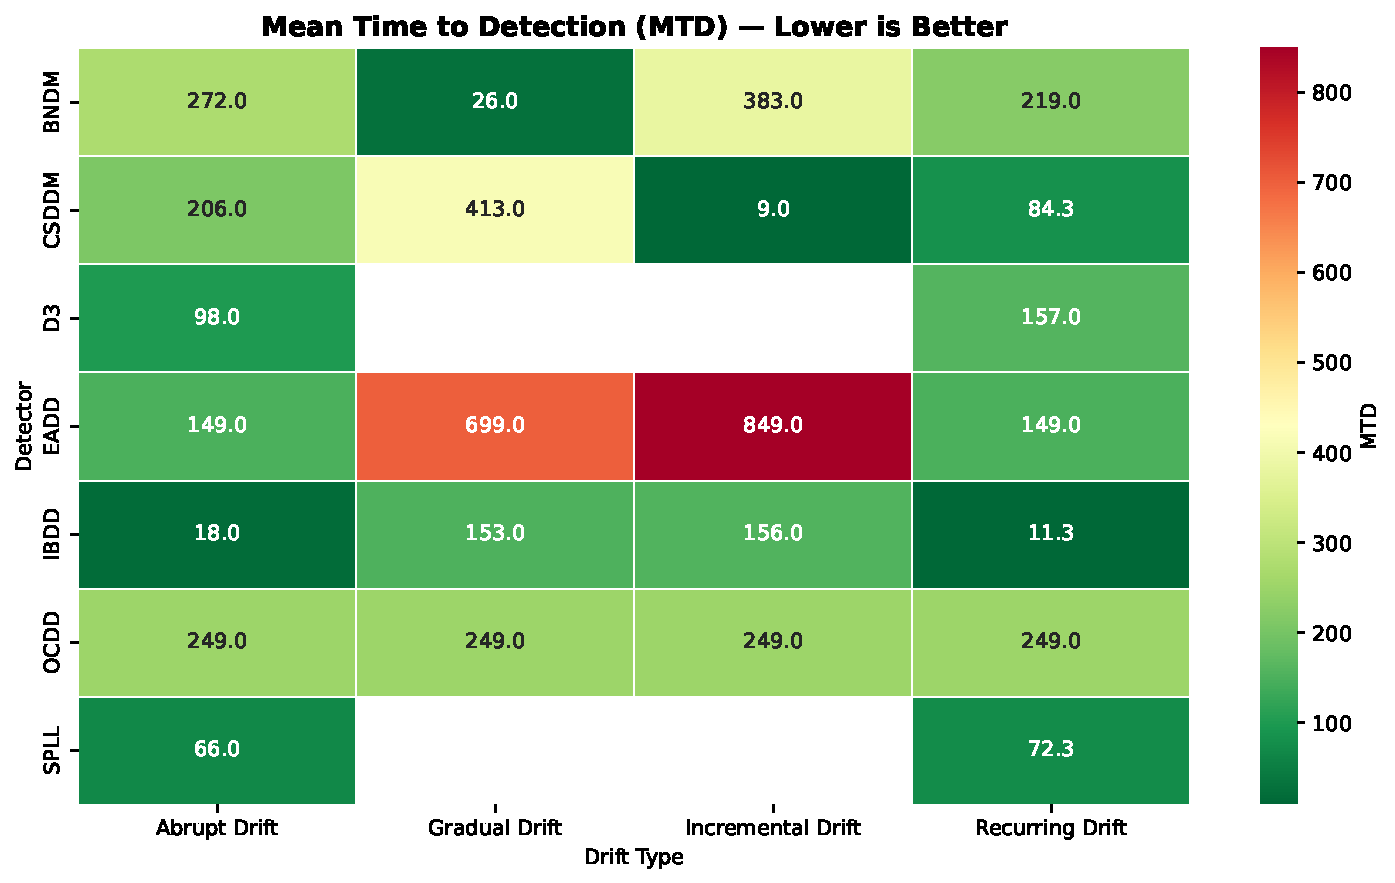
\includegraphics[width=0.86\textwidth,height=0.34\textheight,keepaspectratio]{figures/heatmap_mtd.pdf}\\[0.7em]
    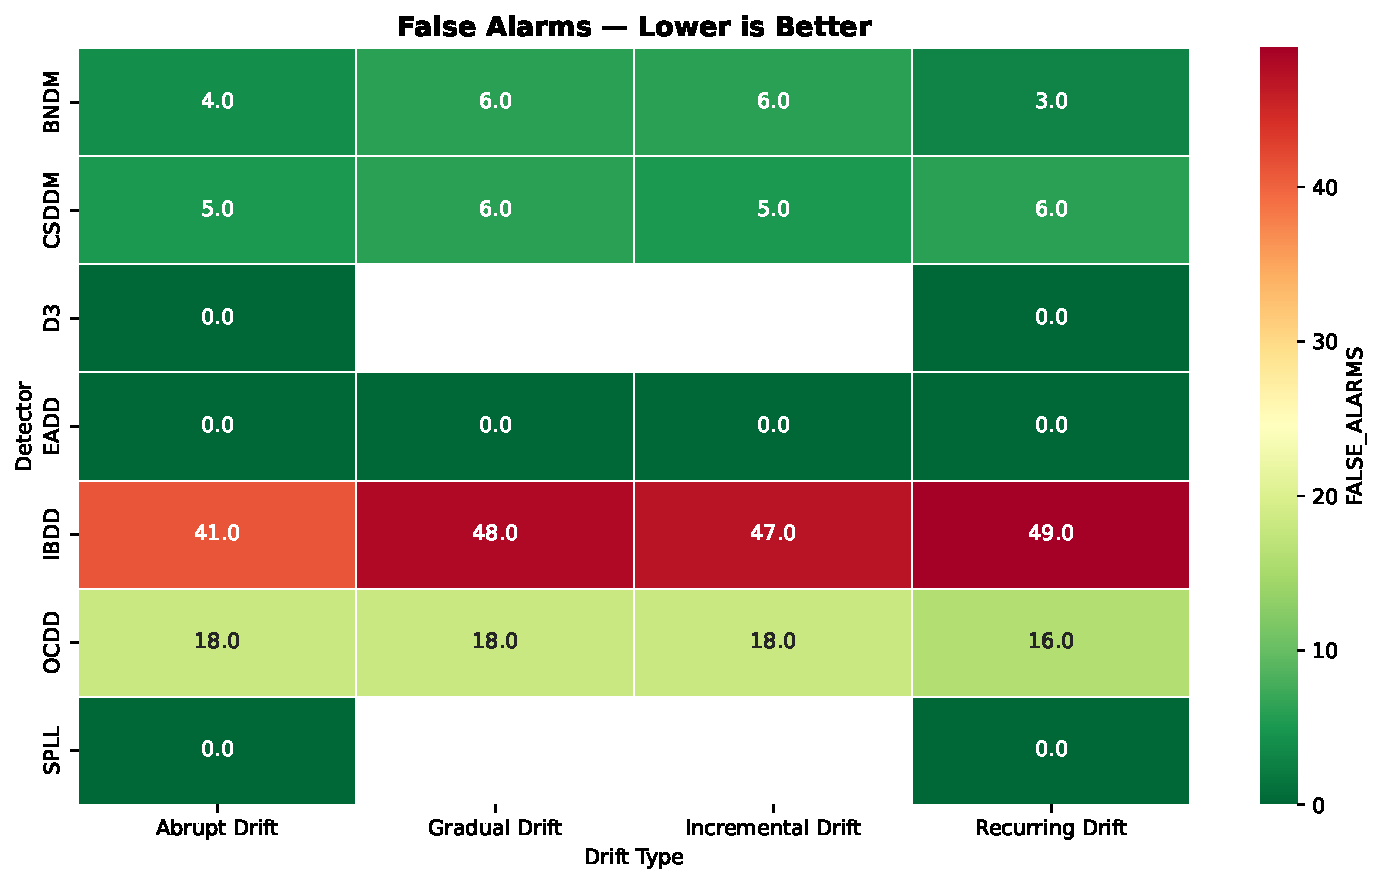
\includegraphics[width=0.86\textwidth,height=0.34\textheight,keepaspectratio]{figures/heatmap_false_alarms.pdf}
    \caption[Heatmaps of detection performance on synthetic drift]{Heatmaps of detection performance on synthetic drift. Top: Mean Time to Detection (lower is better; white cells indicate complete miss). Bottom: False Alarm count (lower is better).}
    \label{fig:heatmap-synthetic}
\end{figure}

Figure~\ref{fig:bell-curves-synthetic} shows the feature distributions before and after drift injection, visualising the distributional shift that each detector must detect.

\begin{figure}[!htbp]
    \centering
    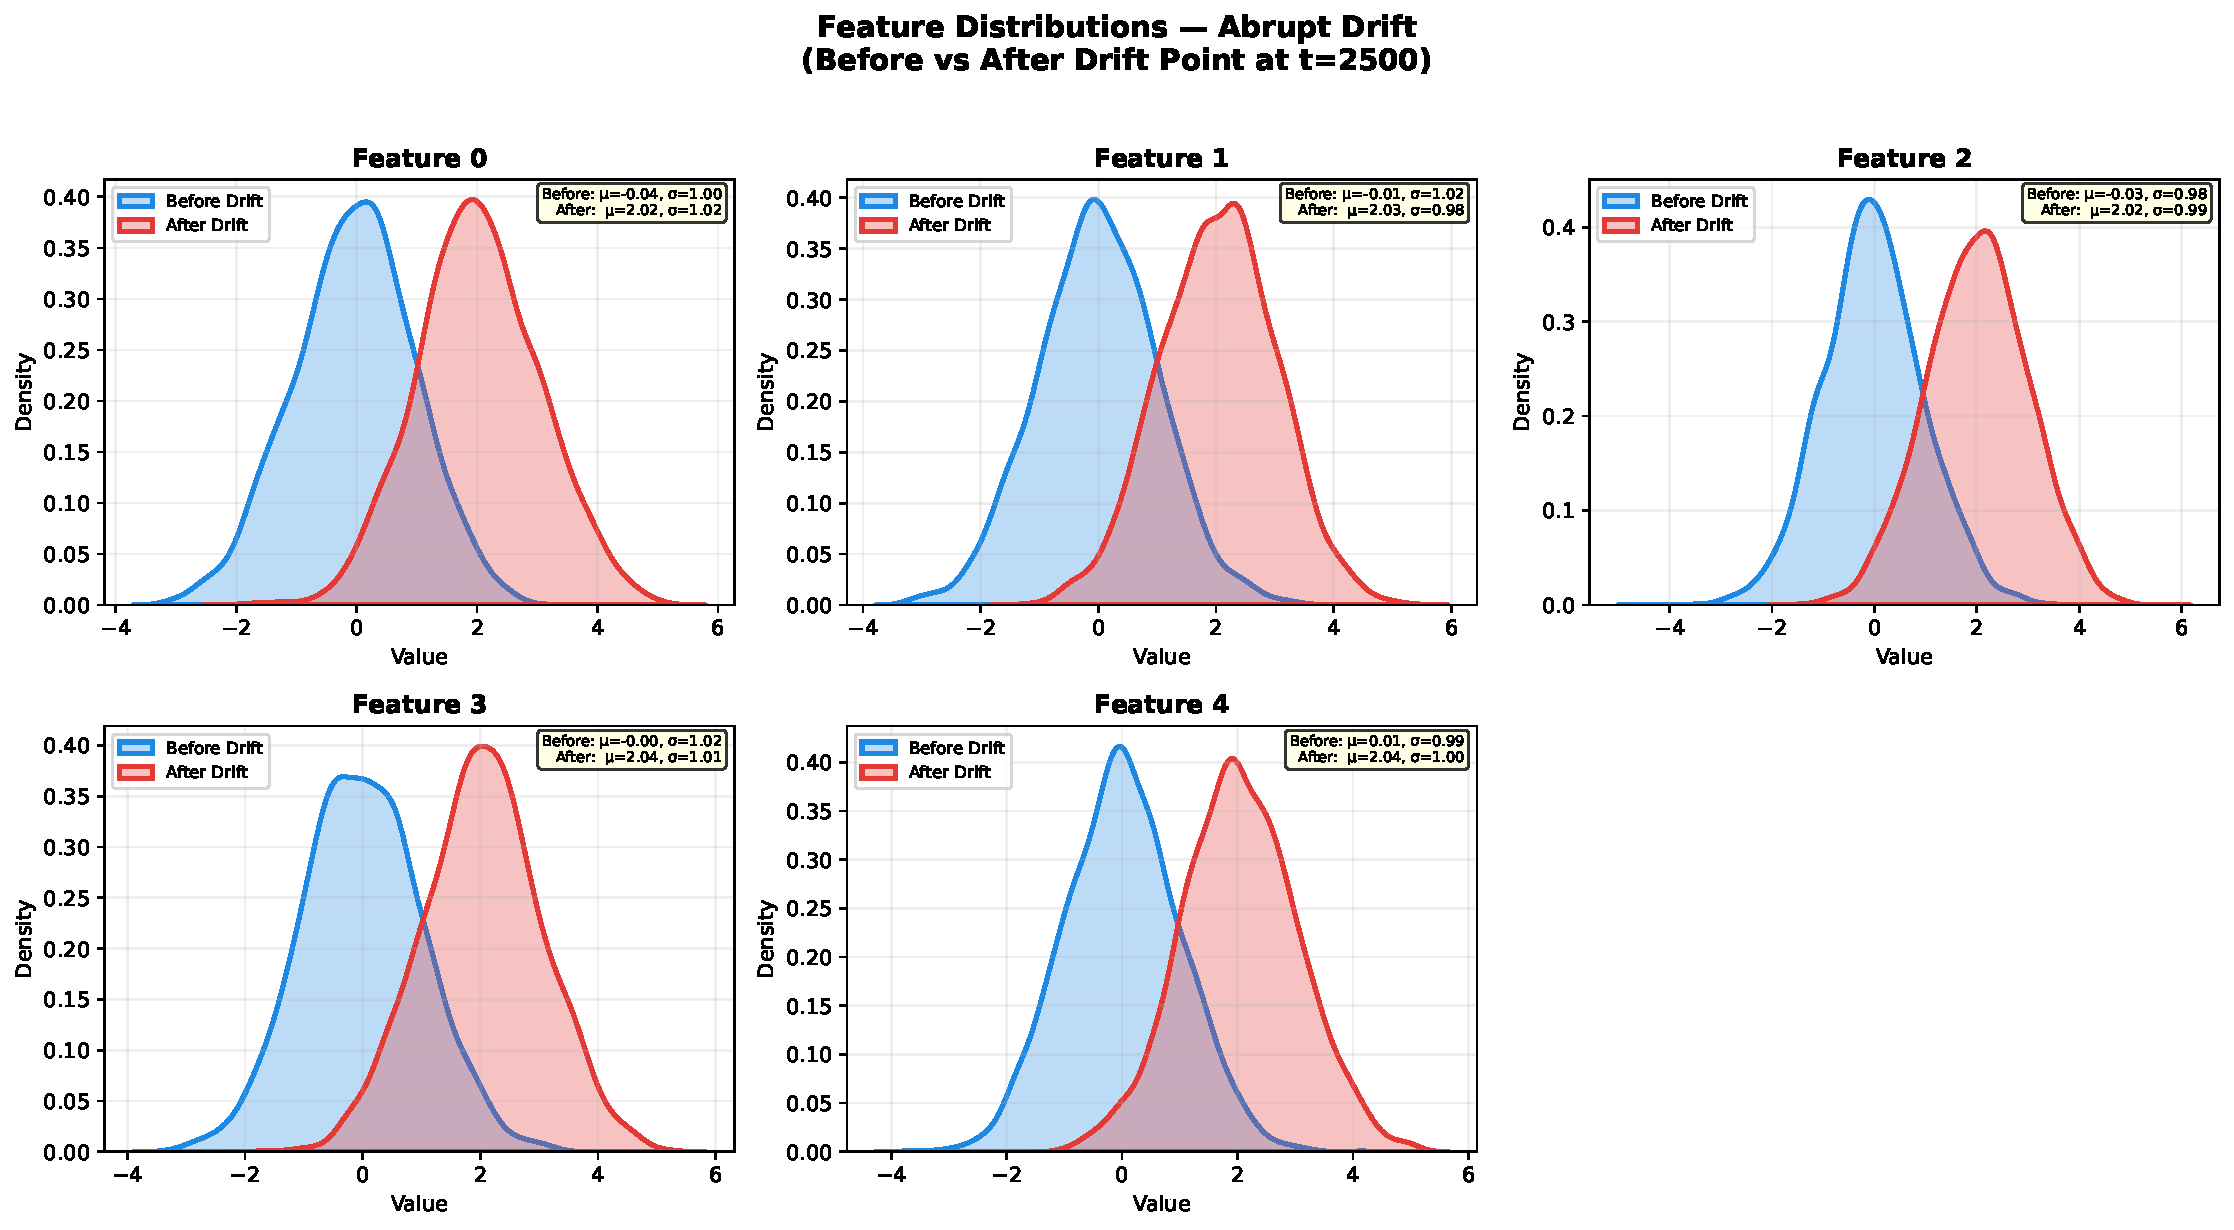
\includegraphics[width=0.86\textwidth,height=0.34\textheight,keepaspectratio]{figures/bell_curves_abrupt_drift.pdf}\\[0.7em]
    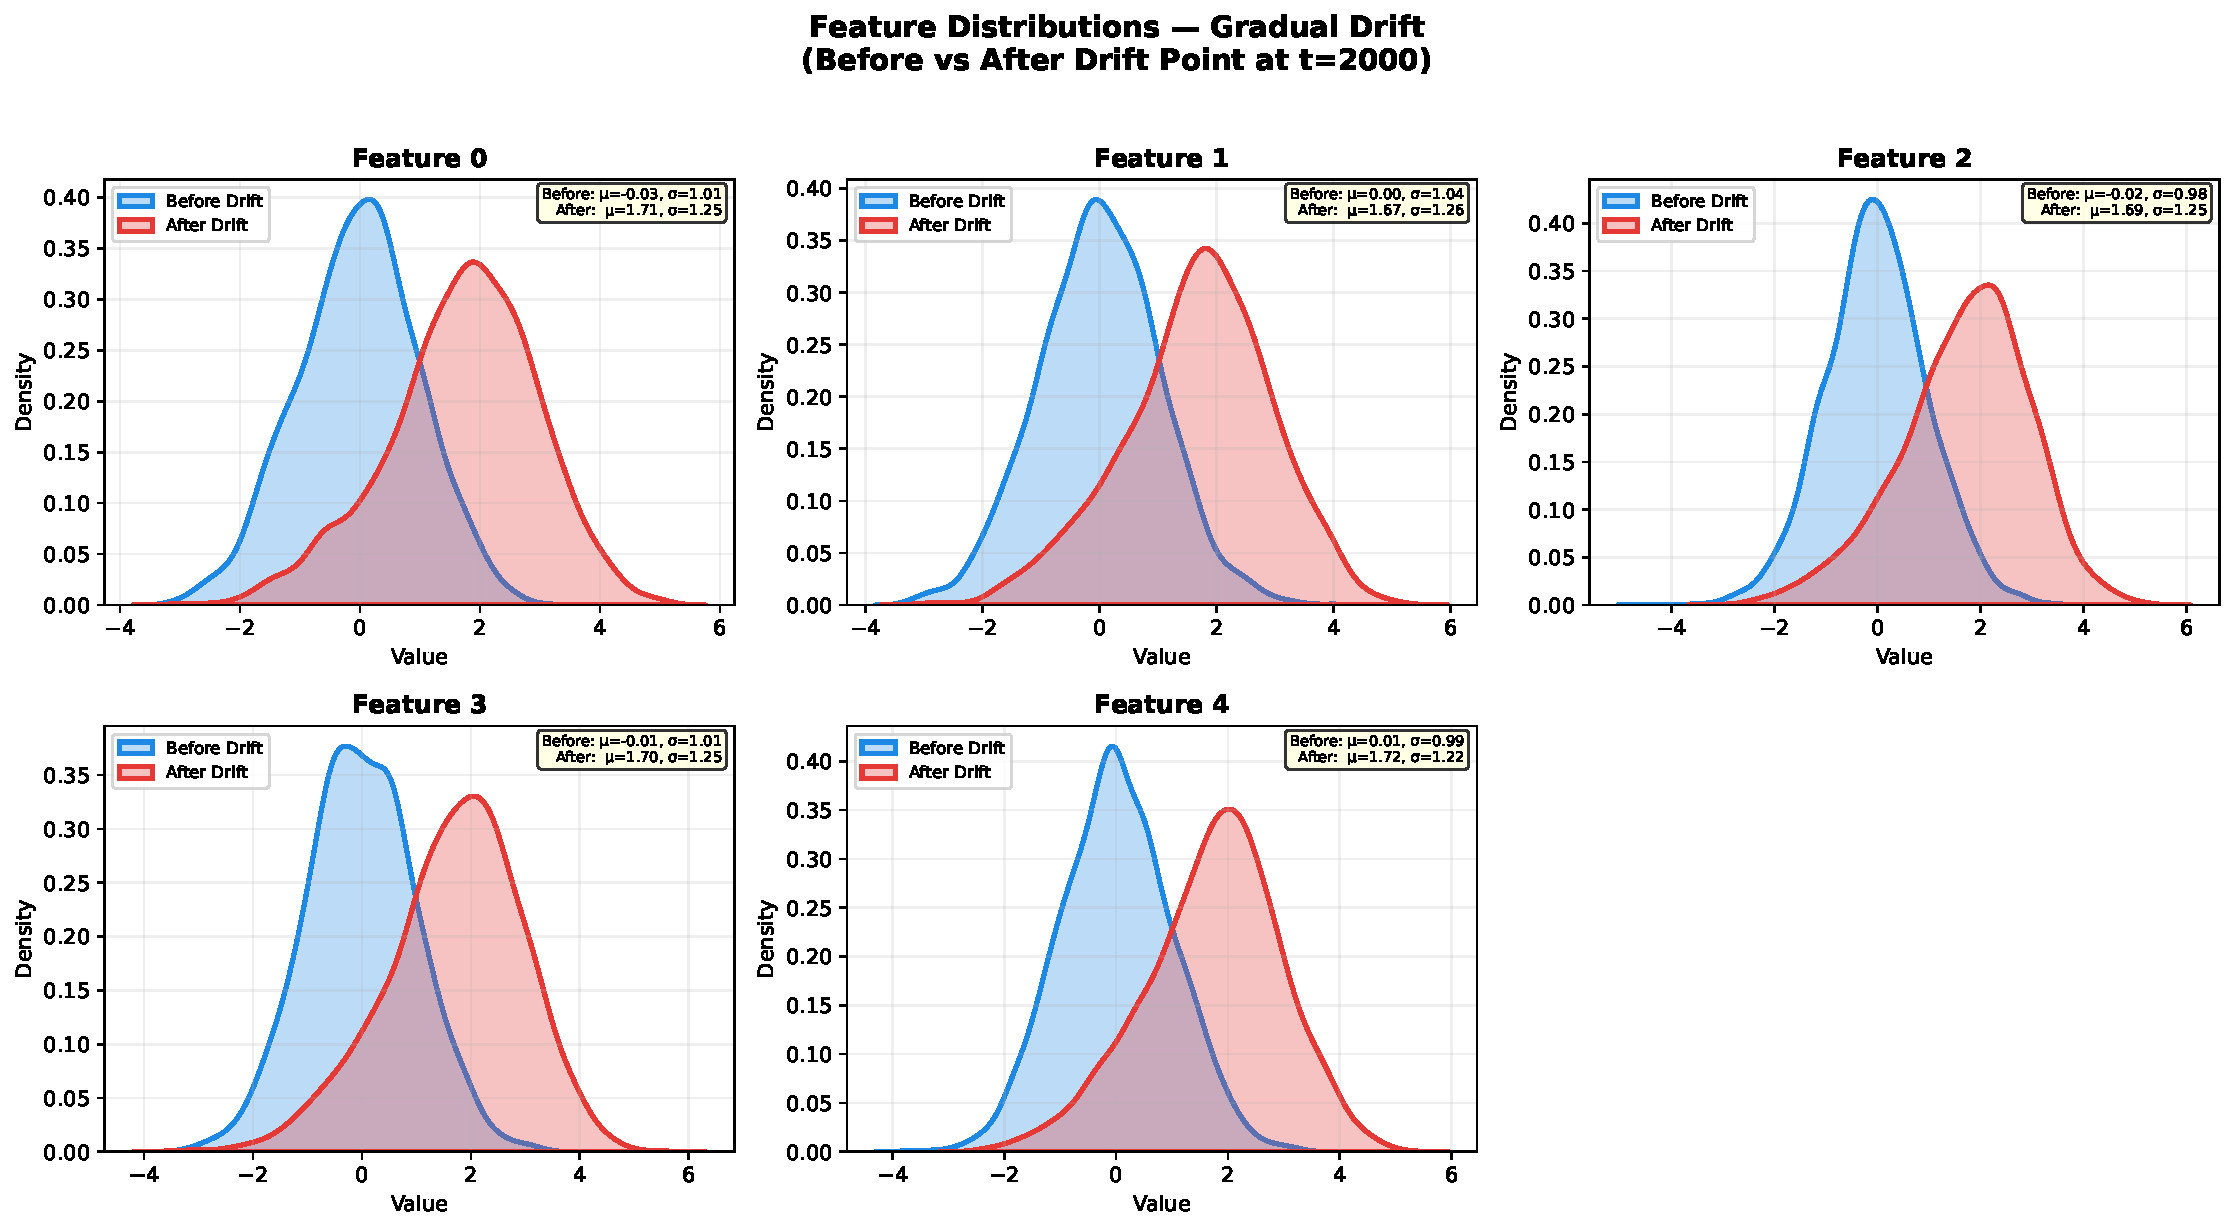
\includegraphics[width=0.86\textwidth,height=0.34\textheight,keepaspectratio]{figures/bell_curves_gradual_drift.pdf}
    \caption[Feature distributions before and after synthetic drift]{Bell curves showing feature distributions before (blue) and after (red) drift injection. Top: Abrupt drift with clear separation. Bottom: Gradual drift with overlapping distributions, the subtle shift that D3, SPLL, and UDetect all failed to detect.}
    \label{fig:bell-curves-synthetic}
\end{figure}

Figure~\ref{fig:timeseries-synthetic} shows the multi-detector time-series comparison, plotting each detector's AUC or detection score over time alongside the true drift point.

\begin{figure}[!htbp]
    \centering
    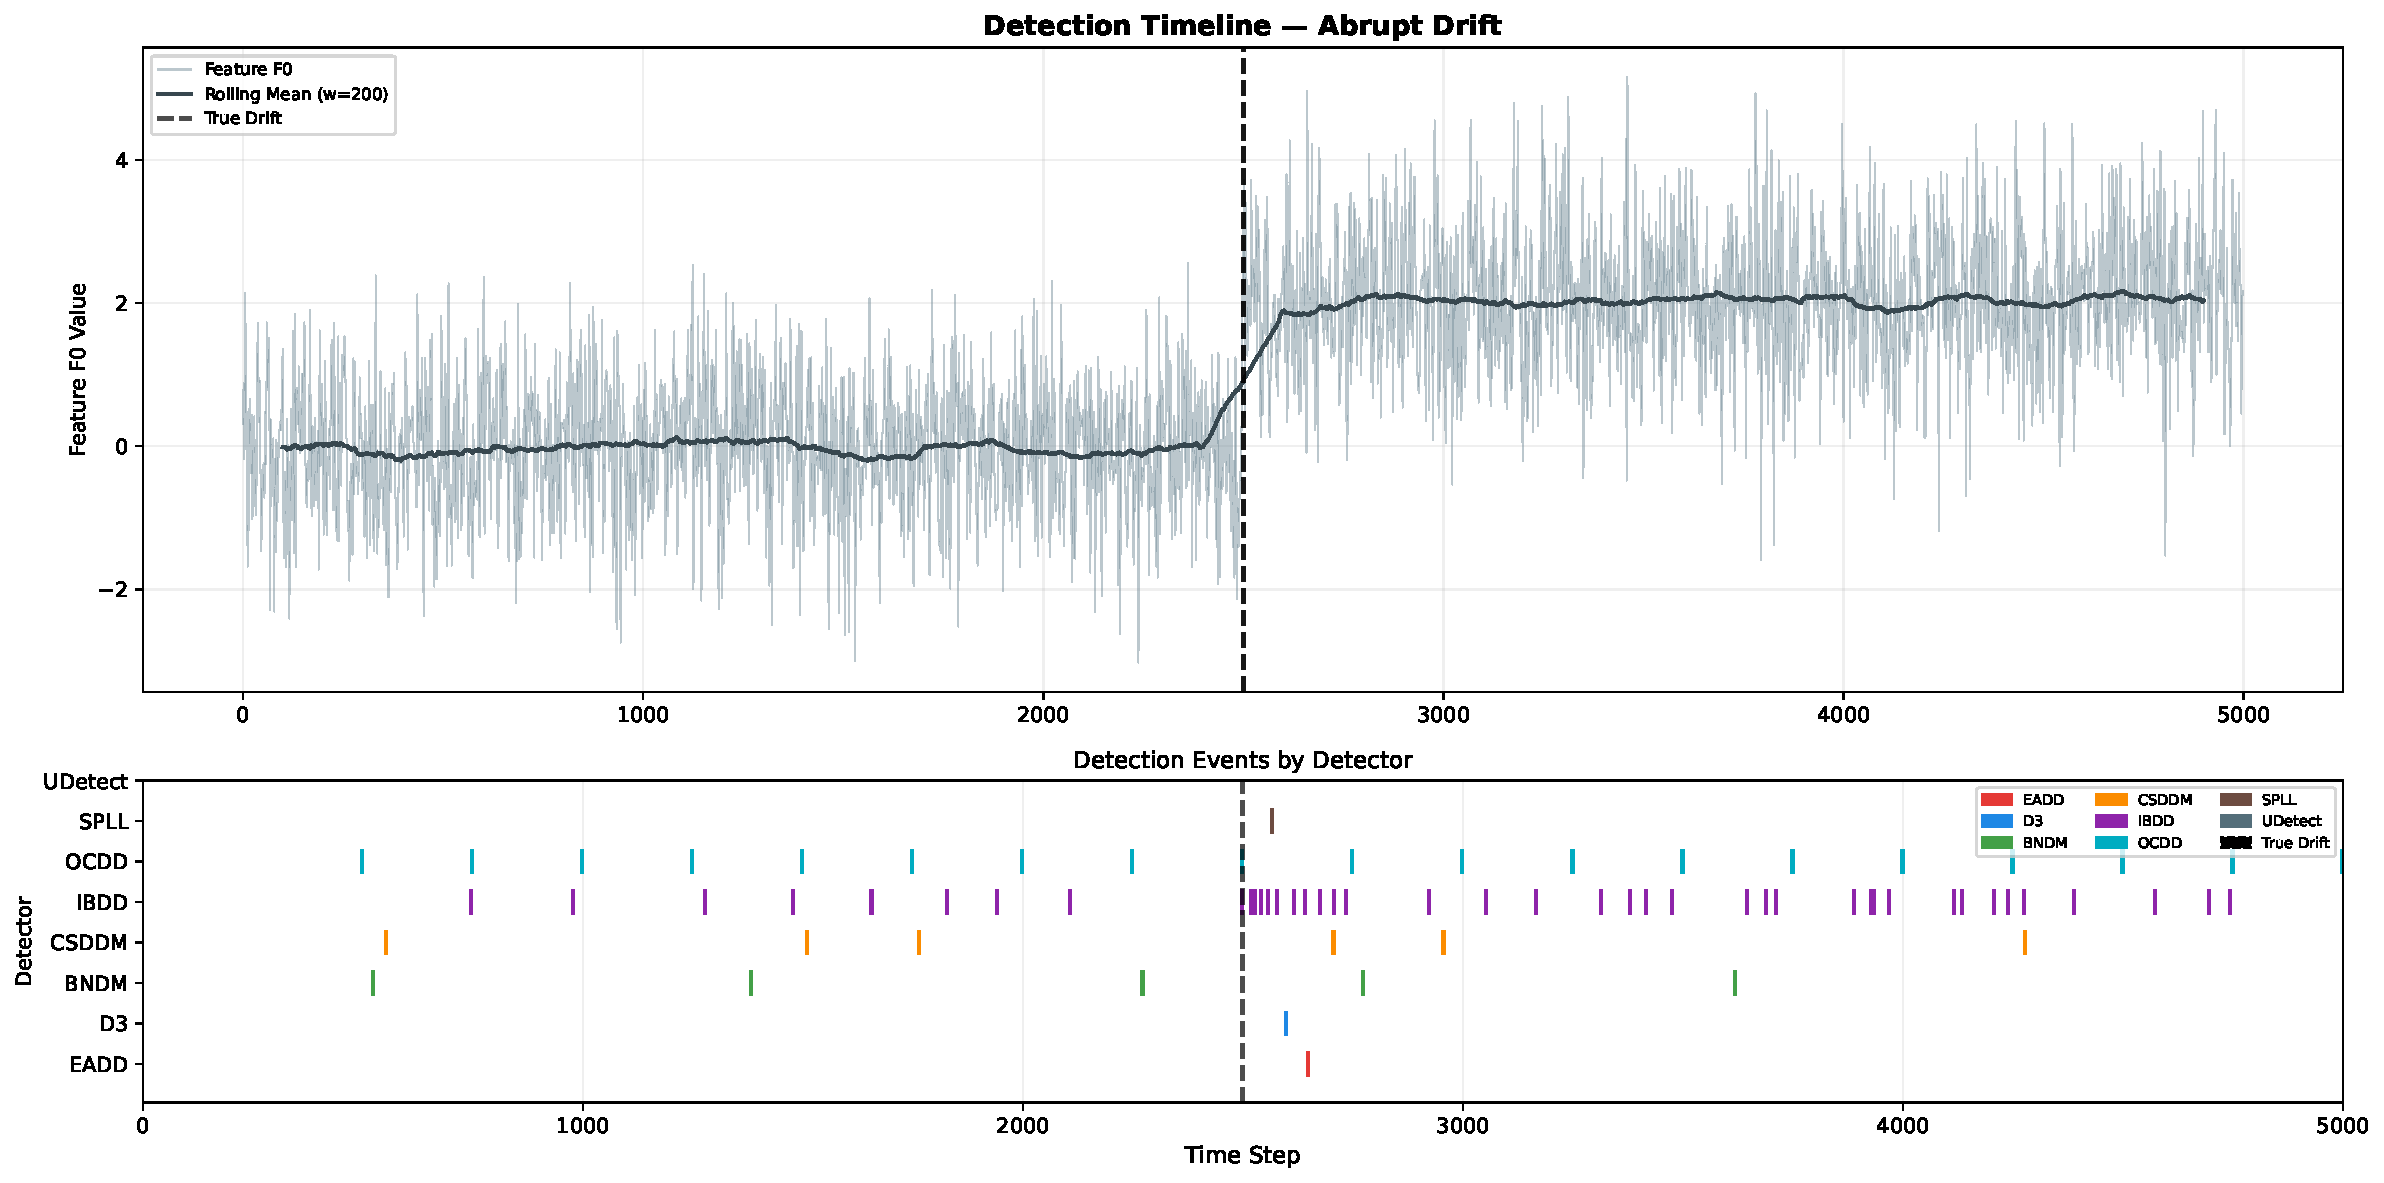
\includegraphics[width=0.86\textwidth,height=0.34\textheight,keepaspectratio]{figures/timeseries_abrupt_drift.pdf}\\[0.7em]
    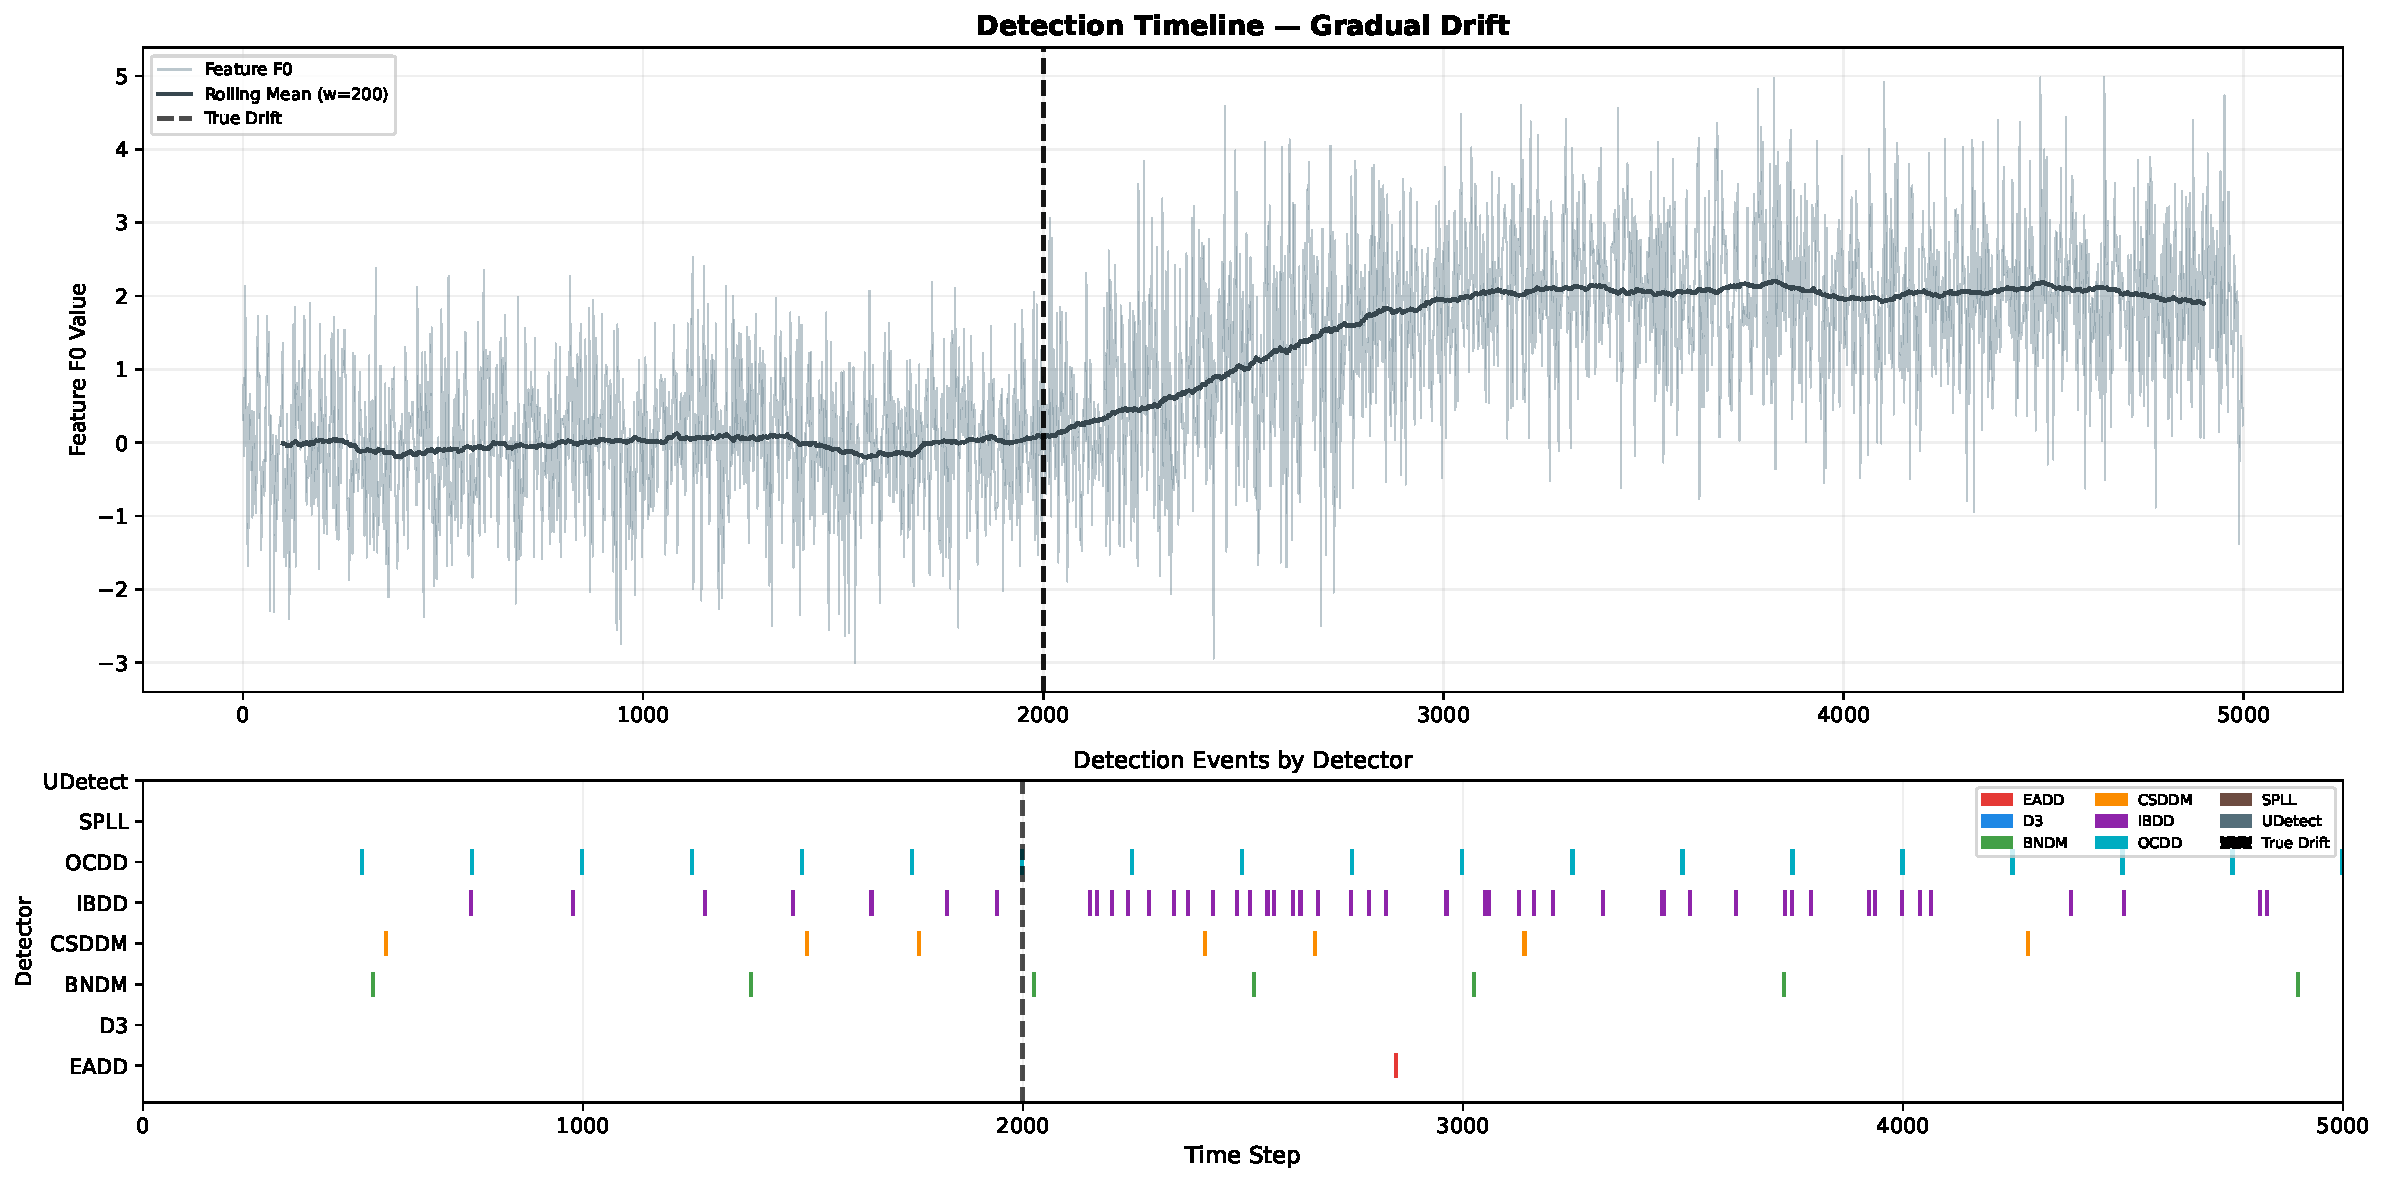
\includegraphics[width=0.86\textwidth,height=0.34\textheight,keepaspectratio]{figures/timeseries_gradual_drift.pdf}
    \caption[Time-series comparison of the eight detectors on synthetic drift]{Time-series comparison of all eight detectors. Top: Abrupt drift; most detectors respond near the true drift point (dashed line). Bottom: Gradual drift; only EADD, BNDM, CSDDM, IBDD, and OCDD detect the shift, while D3, SPLL, and UDetect remain silent.}
    \label{fig:timeseries-synthetic}
\end{figure}

\textbf{Key Findings:}
The multi-detector comparison reveals three groups of detectors:

\begin{enumerate}
    \item \textbf{Complete Coverage without False Alarms:} EADD was the only detector that detected all four drift types (4/4 coverage, MTD: 149--849) with zero false alarms, including the gradual and incremental drift that D3 and SPLL missed entirely. Experiment~4 shows that this coverage comes from EADD's reservoir-sampled reference window rather than from its classifier or its permutation test. EADD's detection delays are longer than those of the fastest detectors (e.g., IBDD's 11--18 samples). EADD also reports a feature ranking with each detection, which the other detectors do not provide.

    \item \textbf{High-Sensitivity Detectors with False Alarm Costs:} BNDM, CSDDM, IBDD, and OCDD also achieved 4/4 drift-type coverage, but with substantially higher false alarm rates (3--49 per drift type). IBDD was the fastest (MTD of 11--18 samples) but generated 41--49 false alarms per type, rendering it impractical for production monitoring. OCDD produced 16--18 false alarms per type with no speed advantage over EADD.

    \item \textbf{Missed Drift Types:} D3 and SPLL both missed gradual and incremental drift entirely (MDR = 1.0), detecting only 2/4 types. UDetect failed on all four types.
\end{enumerate}

\section{Experiment 2: Real-World Benchmark}
\label{sec:exp2}

\textbf{Objective:} Evaluate EADD and the baseline detectors on real-world data streams from the \citet{Lukats2024} benchmark, where drift patterns are unknown, complex, and multi-dimensional.

\textbf{Procedure:}
Thirteen real-world datasets (Section~\ref{sec:datasets}) were processed in streaming fashion by EADD and D3, with D3 using the same window sizes as EADD, for up to 100{,}000 samples per stream and with three seeds (42, 142 and 242). For the four annotated datasets (InsectsAbrupt, InsectsGradual, InsectsIncrAbrupt, InsectsIncrRecur), precision, recall and MTD were computed against the known drift points, with a detection counted as correct if it occurred within 500 samples after a drift point. For the nine unannotated datasets, the total number of detections was recorded as a selectivity indicator.

A supplementary multi-detector run compared all eight detectors on the first 20{,}000 samples of an 11-stream subset of the same benchmark (excluding Luxembourg, Ozone, PokerHand and RialtoBridge). A per-detector timeout of 120 seconds was applied in this run, as BNDM's computation exceeded practical limits on the 33-feature INSECTS datasets.

\textbf{Results:}

Table~\ref{tab:exp2-results} presents the results on datasets with known drift points.

\begin{table}[!htbp]
\centering
\caption[Experiment 2: EADD vs.\ D3 on annotated real-world datasets]{Experiment 2: EADD vs.\ D3 on the four annotated real-world datasets, averaged over three seeds. MTD = Mean Time to Detection (samples; lower is better). Bold indicates that EADD outperforms D3. ``--'' = all known drift points missed. Low precision on incremental datasets reflects the INSECTS annotation convention: only major transition boundaries are annotated; additional detections may correspond to unannotated continuous incremental changes rather than false alarms.}
\label{tab:exp2-results}
\begin{tabular}{l|cc|cc|cc}
\hline
 & \multicolumn{2}{c|}{\textbf{Precision}} & \multicolumn{2}{c|}{\textbf{Recall}} & \multicolumn{2}{c}{\textbf{MTD}} \\
\textbf{Dataset} & EADD & D3 & EADD & D3 & EADD & D3 \\
\hline
InsectsAbrupt     & 0.33 & 0.41 & 0.60 & 0.73 & \textbf{124} & 166 \\
InsectsGradual    & 0.00 & 0.00 & 0.00 & 0.00 & --           & --  \\
InsectsIncrAbrupt & 0.14 & 0.29 & 1.00 & 1.00 & \textbf{50}  & 126 \\
InsectsIncrRecur  & 0.12 & 0.18 & 0.83 & 1.00 & \textbf{84}  & 256 \\
\hline
\end{tabular}
\end{table}

Table~\ref{tab:exp2-nogt} summarises detection activity on the nine unannotated datasets.

\begin{table}[!htbp]
\centering
\caption[Experiment 2: detection counts on unannotated datasets]{Experiment 2: Mean number of detections over three seeds on the nine unannotated real-world datasets (EADD vs.\ D3). Ground-truth drift counts are unknown; counts indicate detection activity, not false alarm rates.}
\label{tab:exp2-nogt}
\begin{tabular}{lcc}
\hline
\textbf{Dataset} & \textbf{EADD} & \textbf{D3} \\
\hline
Electricity & 90.0 & 86.0 \\
INSECTS Incremental & 1.0 & 0.7 \\
Luxembourg & 3.0 & 1.0 \\
NOAAWeather & 12.7 & 29.7 \\
OutdoorObjects & 6.0 & 1.0 \\
Ozone & 1.0 & 4.0 \\
PokerHand & 199.0 & 193.0 \\
Powersupply & 10.0 & 18.3 \\
RialtoBridge & 152.0 & 138.0 \\
\hline
\textbf{Total} & \textbf{474.7} & \textbf{471.7} \\
\hline
\end{tabular}
\end{table}

\textbf{Multi-Detector Context (11-stream subset):}
Table~\ref{tab:exp2-multidet} presents the supplementary multi-detector comparison, including the semi-synthetic benchmarks SineClusters and WaveformDrift2, which have annotated drift points in the \citet{Lukats2024} framework. Because this run used only the first 20{,}000 samples of each stream and a single run, its values for EADD and D3 differ from those in Table~\ref{tab:exp2-results}.

\begin{table}[!htbp]
\centering
\caption[Experiment 2: supplementary multi-detector comparison]{Supplementary multi-detector comparison on the first 20{,}000 samples of the annotated streams in the 11-stream subset. MTD = Mean Time to Detection (samples); bold marks the lowest MTD per stream. ``--'' = detector missed all annotated drifts or timed out. MTD ignores false alarms: IBDD, for example, raised 72 detections on InsectsAbrupt.}
\label{tab:exp2-multidet}
\begin{tabular}{l|c|c|c|c}
\hline
\textbf{Detector} & \textbf{InsectsAbrupt} & \textbf{InsectsGradual} & \textbf{SineClusters} & \textbf{WaveformDrift2} \\
\hline
EADD & 148 & -- & 299 & 99 \\
D3 & 152.5 & -- & 219 & 179 \\
BNDM & -- & -- & 499 & 60 \\
CSDDM & 44 & 143 & \textbf{35} & 359 \\
IBDD & 28 & 88 & 45 & \textbf{8} \\
OCDD & 254 & -- & 249 & 249 \\
SPLL & \textbf{25} & \textbf{39} & 249 & 22 \\
UDetect & -- & -- & 36 & 21 \\
\hline
\end{tabular}
\end{table}

Figure~\ref{fig:heatmap-realworld} presents heatmaps summarising detection performance across all detector and dataset combinations of the supplementary run.

\begin{figure}[!htbp]
    \centering
    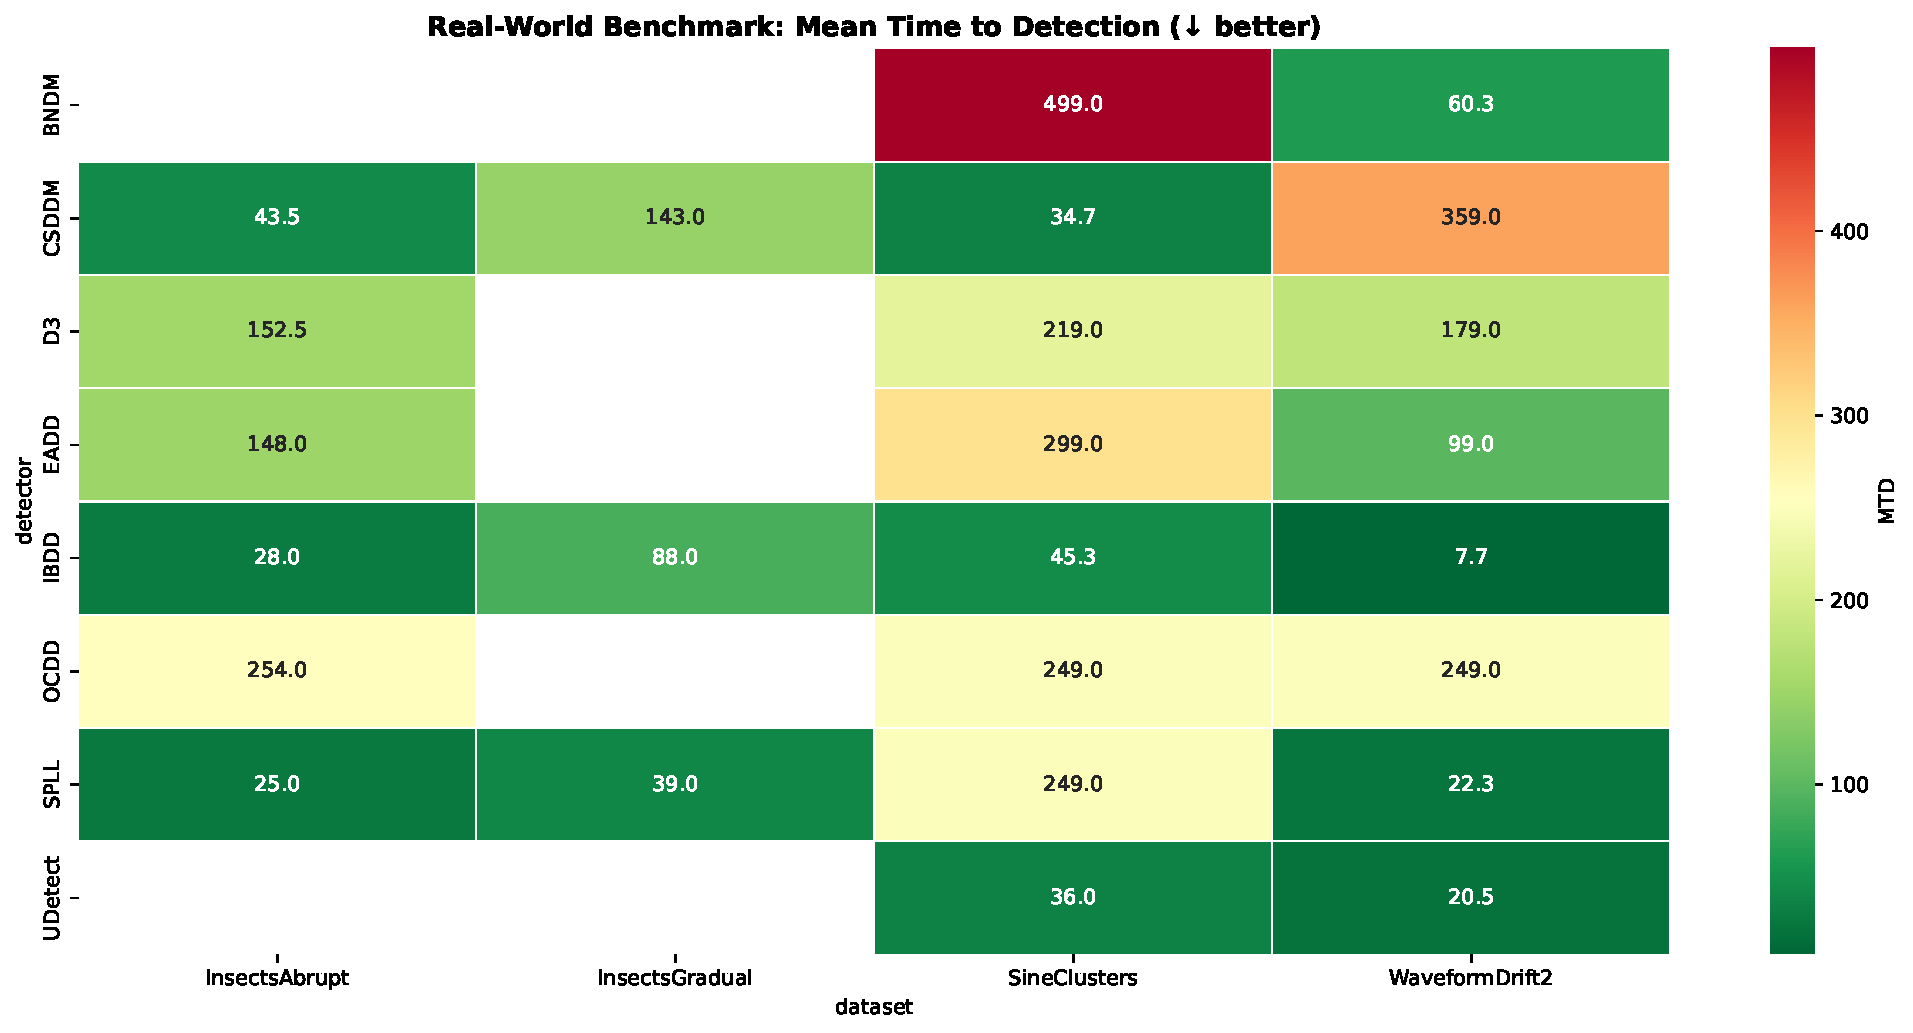
\includegraphics[width=0.86\textwidth,height=0.34\textheight,keepaspectratio]{figures/heatmap_realworld_mtd.pdf}\\[0.7em]
    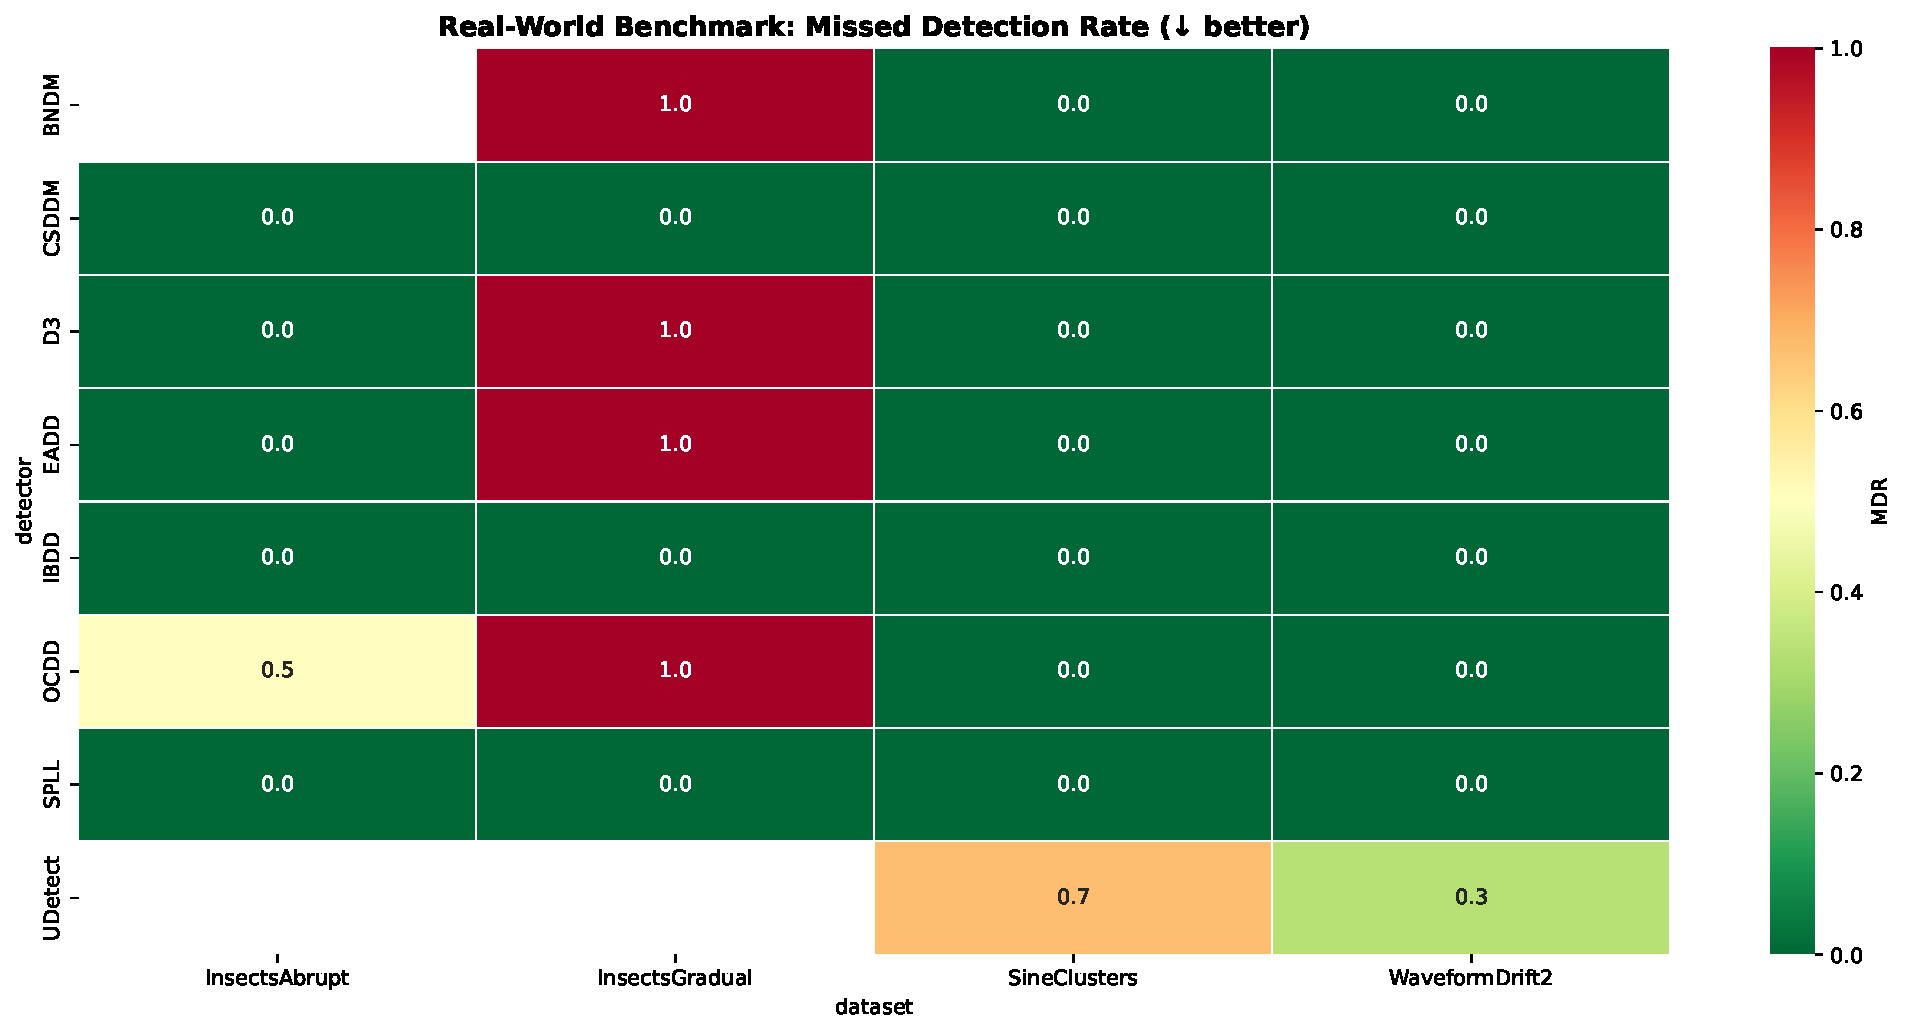
\includegraphics[width=0.86\textwidth,height=0.34\textheight,keepaspectratio]{figures/heatmap_realworld_mdr.pdf}
    \caption[Heatmaps of the multi-detector real-world run]{Heatmaps of the supplementary multi-detector real-world run. Top: Mean Time to Detection (lower is better; white cells indicate missed drifts or timeout). Bottom: Missed Detection Rate (0.0 is perfect).}
    \label{fig:heatmap-realworld}
\end{figure}

Figure~\ref{fig:timeseries-realworld} shows time-series visualisations of detection behaviour on two semi-synthetic datasets.

\begin{figure}[!htbp]
    \centering
    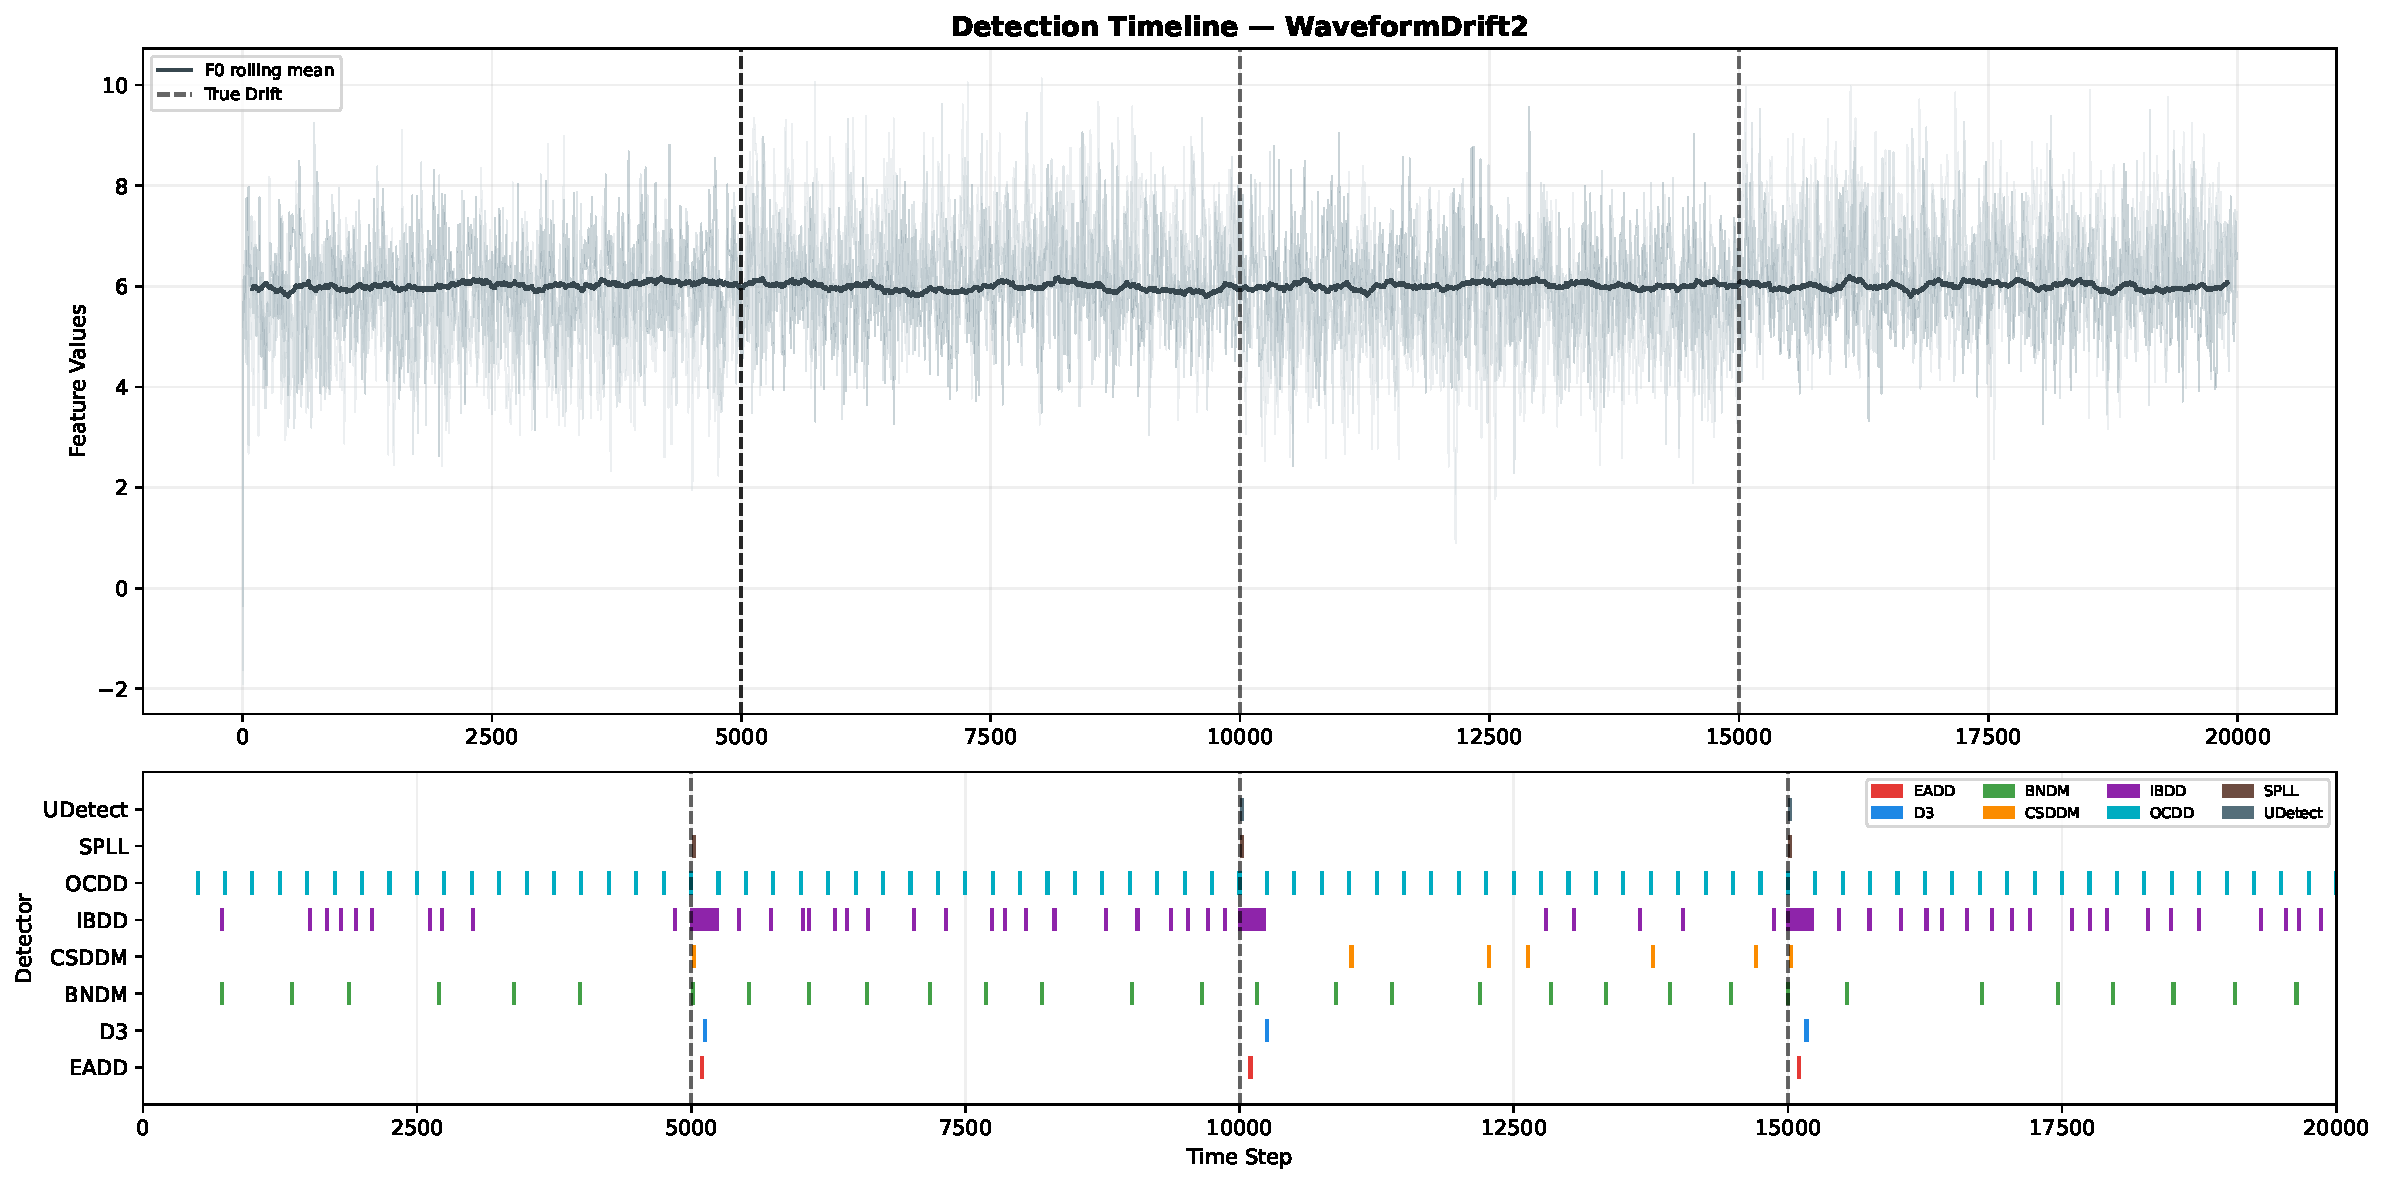
\includegraphics[width=0.86\textwidth,height=0.34\textheight,keepaspectratio]{figures/timeseries_realworld_waveformdrift2.pdf}\\[0.7em]
    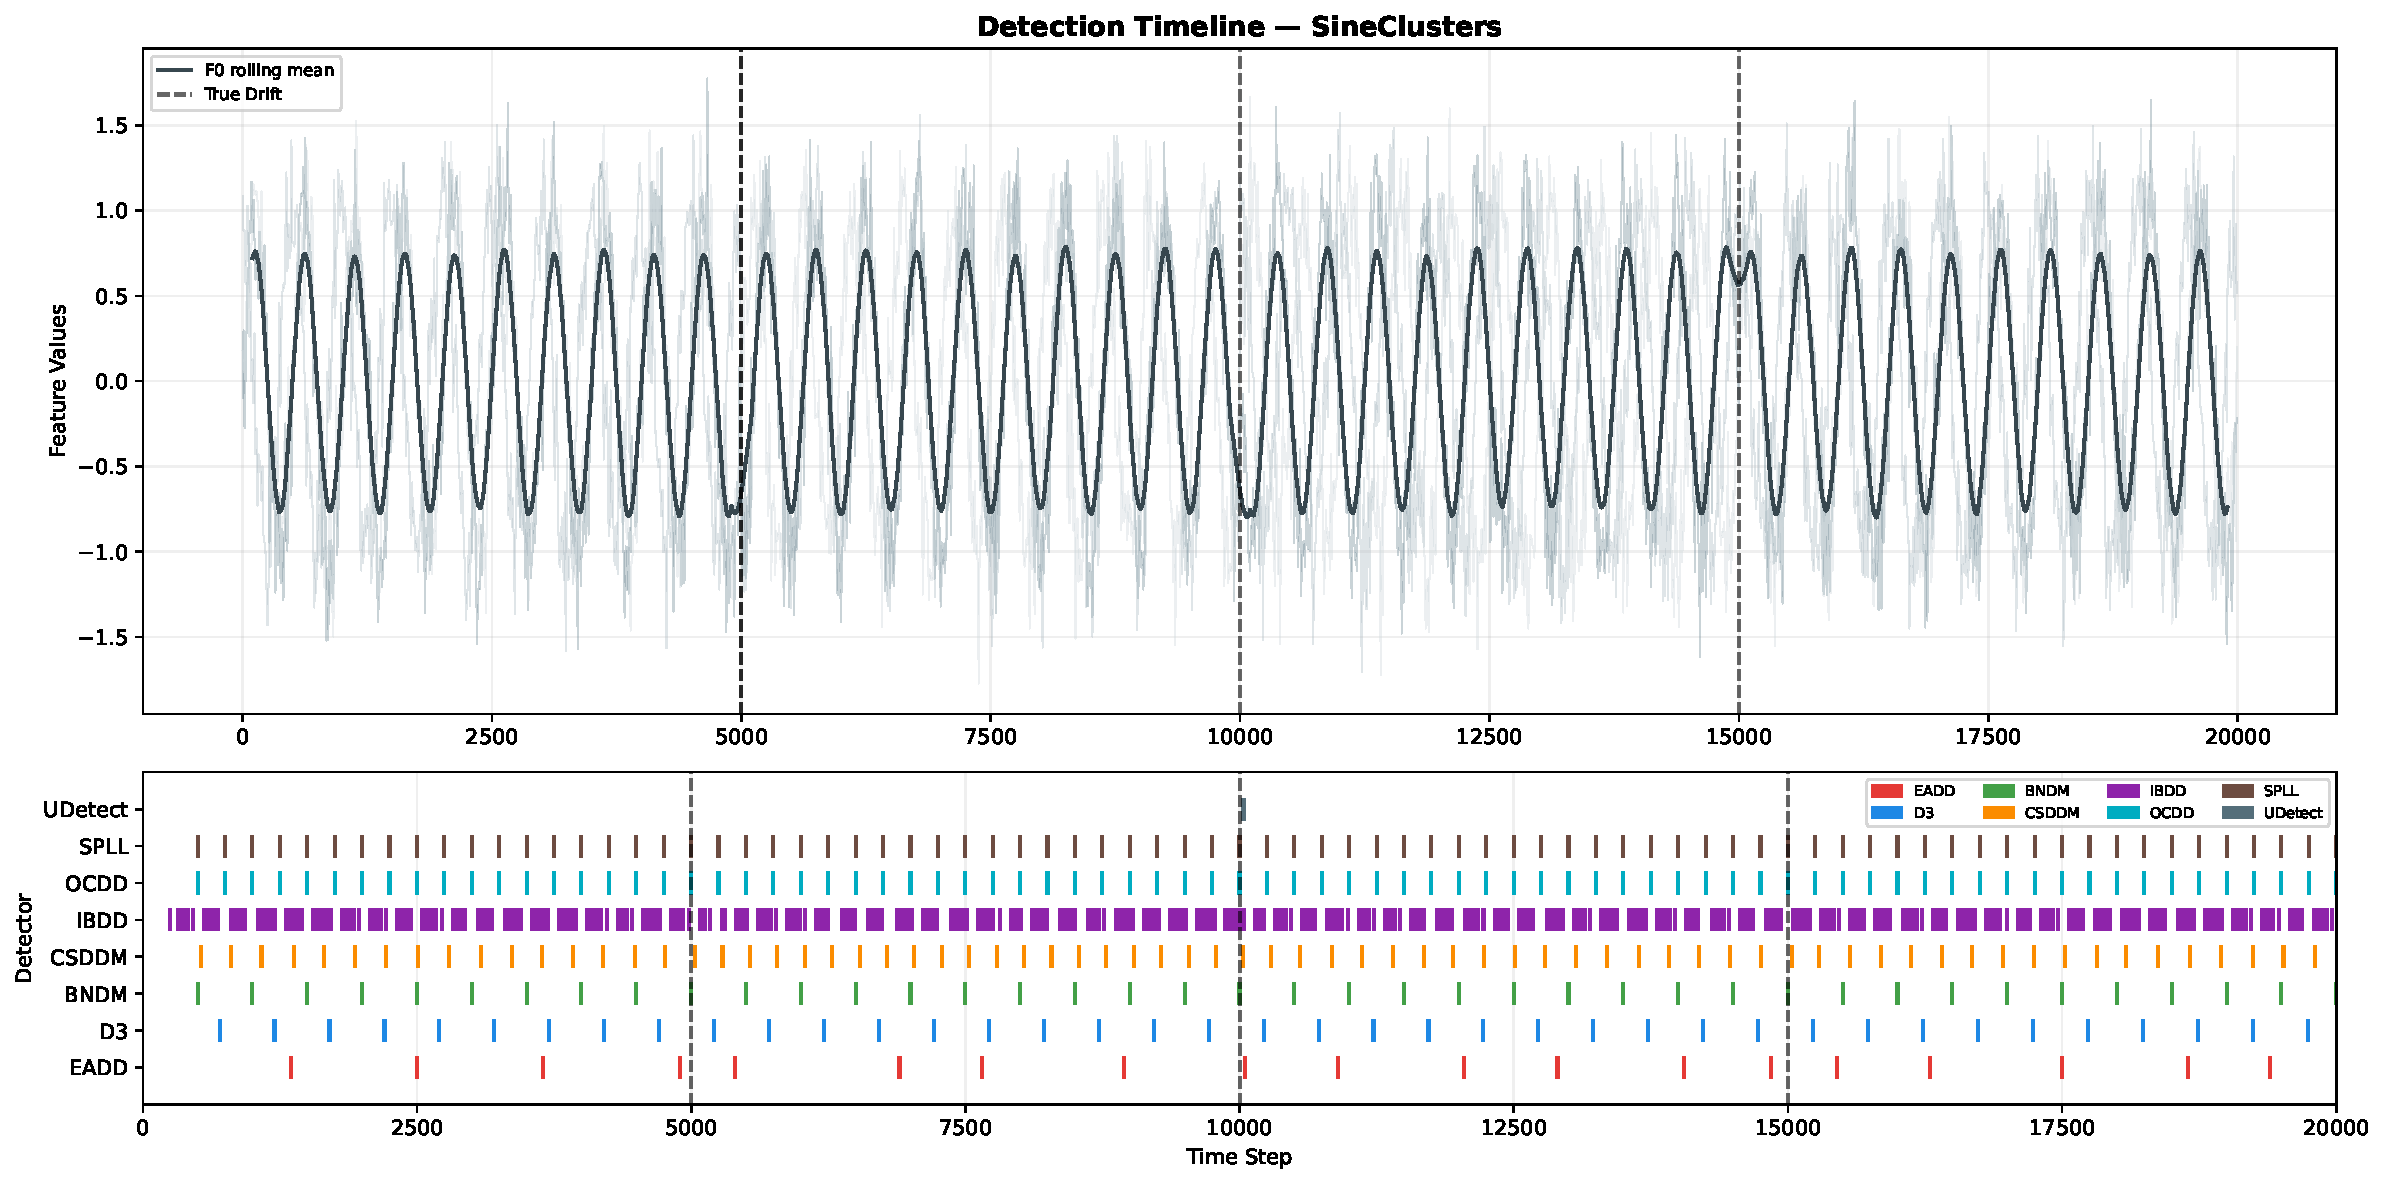
\includegraphics[width=0.86\textwidth,height=0.34\textheight,keepaspectratio]{figures/timeseries_realworld_sineclusters.pdf}
    \caption[Time-series comparison on semi-synthetic benchmark datasets]{Time-series comparison on benchmark datasets from the multi-detector supplementary run. Top: WaveformDrift2 (semi-synthetic); EADD detects all three drift points (MTD=99), faster than D3 (MTD=179). Bottom: SineClusters (semi-synthetic); IBDD detects rapidly but with many excess detections, illustrating the sensitivity and specificity trade-off.}
    \label{fig:timeseries-realworld}
\end{figure}

Figure~\ref{fig:bell-curves-realworld} shows the feature distributions for representative real-world datasets, illustrating the distributional complexity that detectors must handle.

\begin{figure}[!htbp]
    \centering
    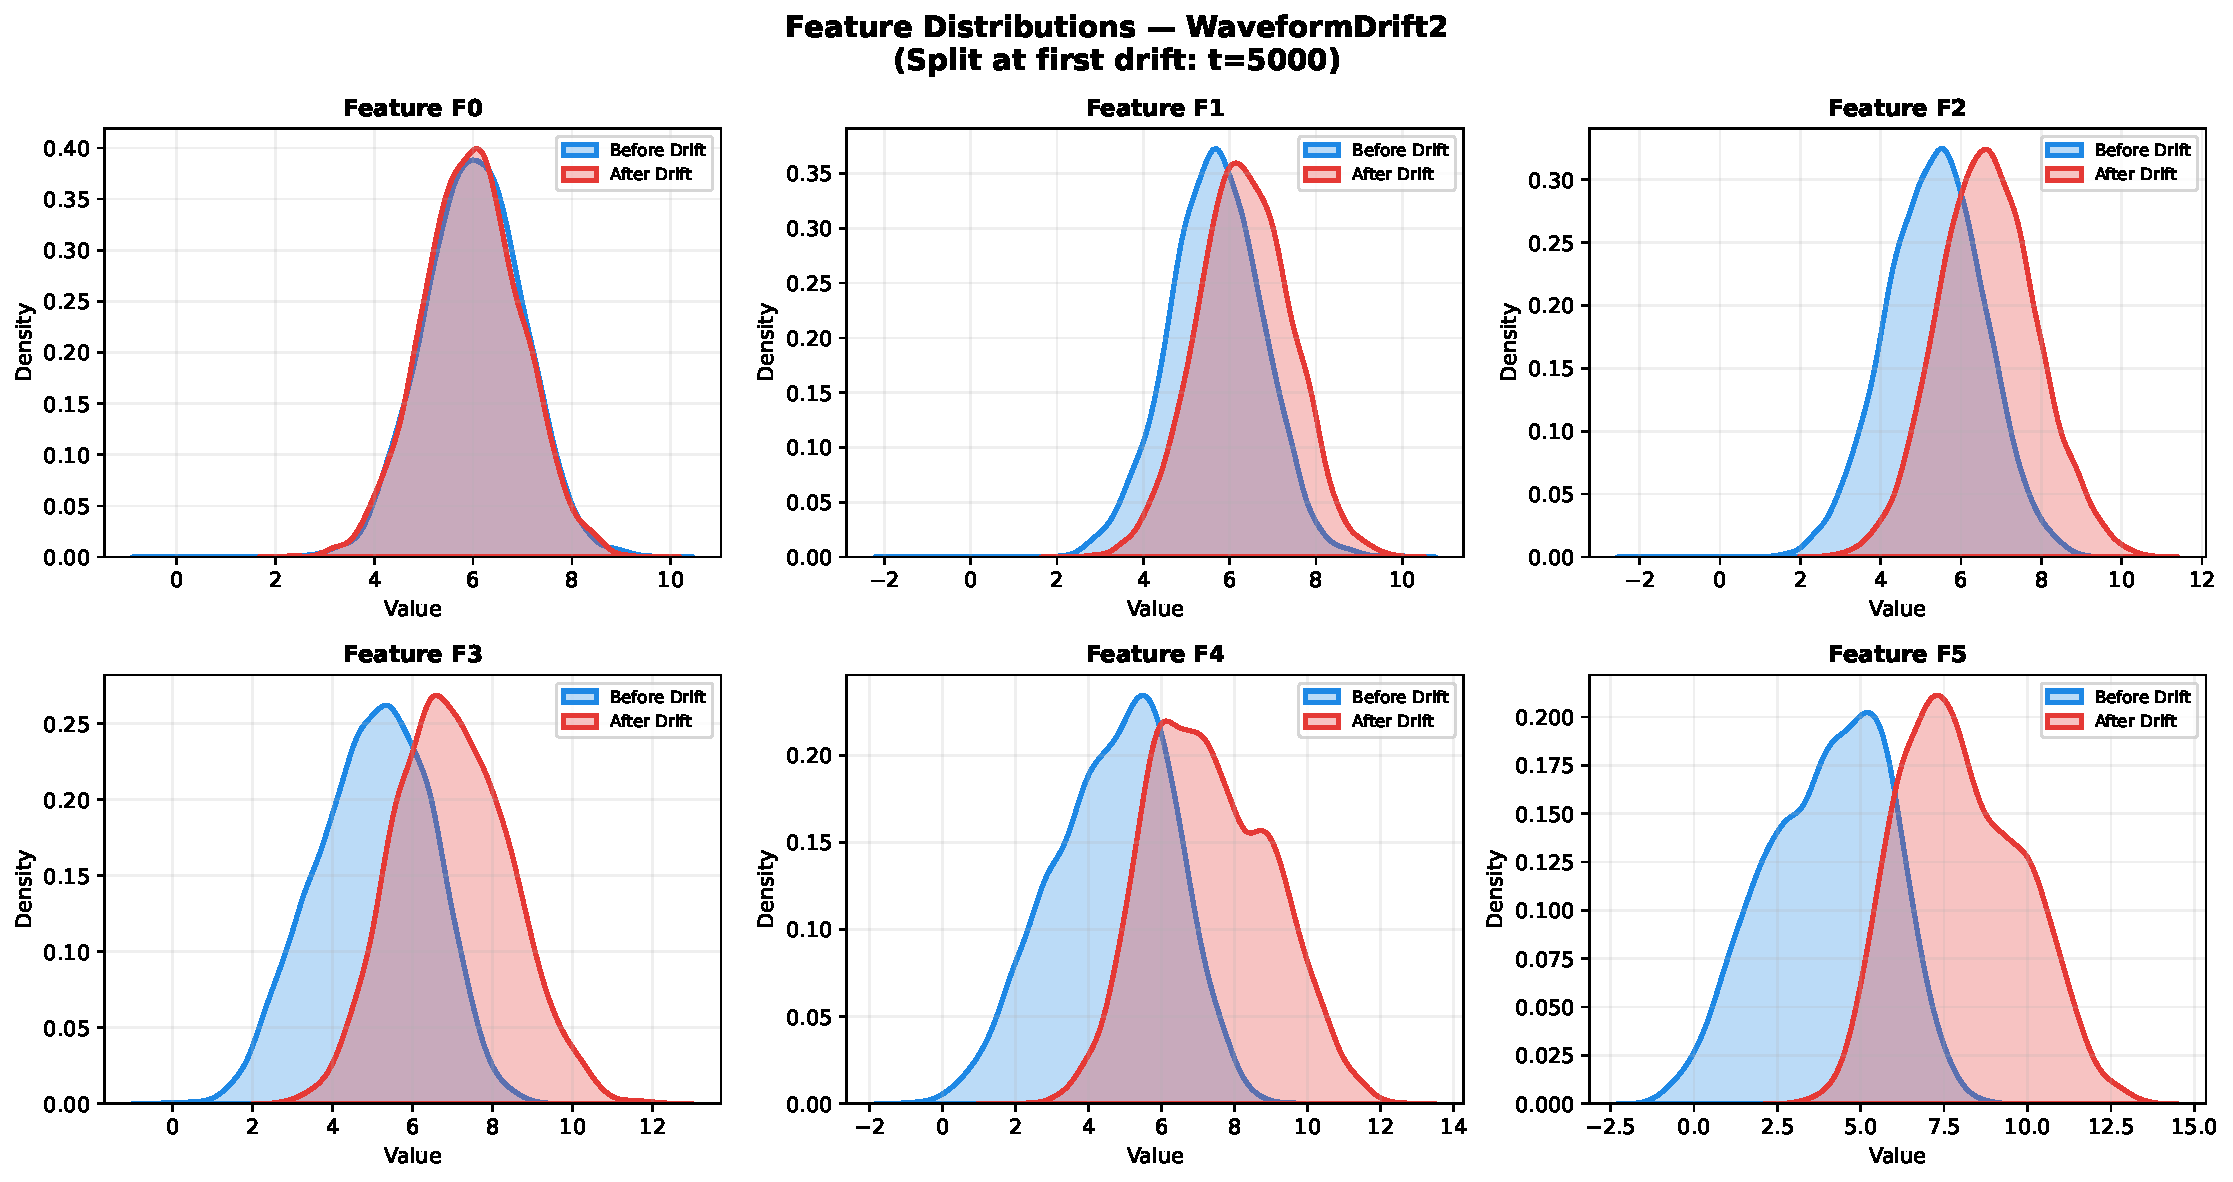
\includegraphics[width=0.86\textwidth,height=0.34\textheight,keepaspectratio]{figures/bell_curves_realworld_waveformdrift2.pdf}\\[0.7em]
    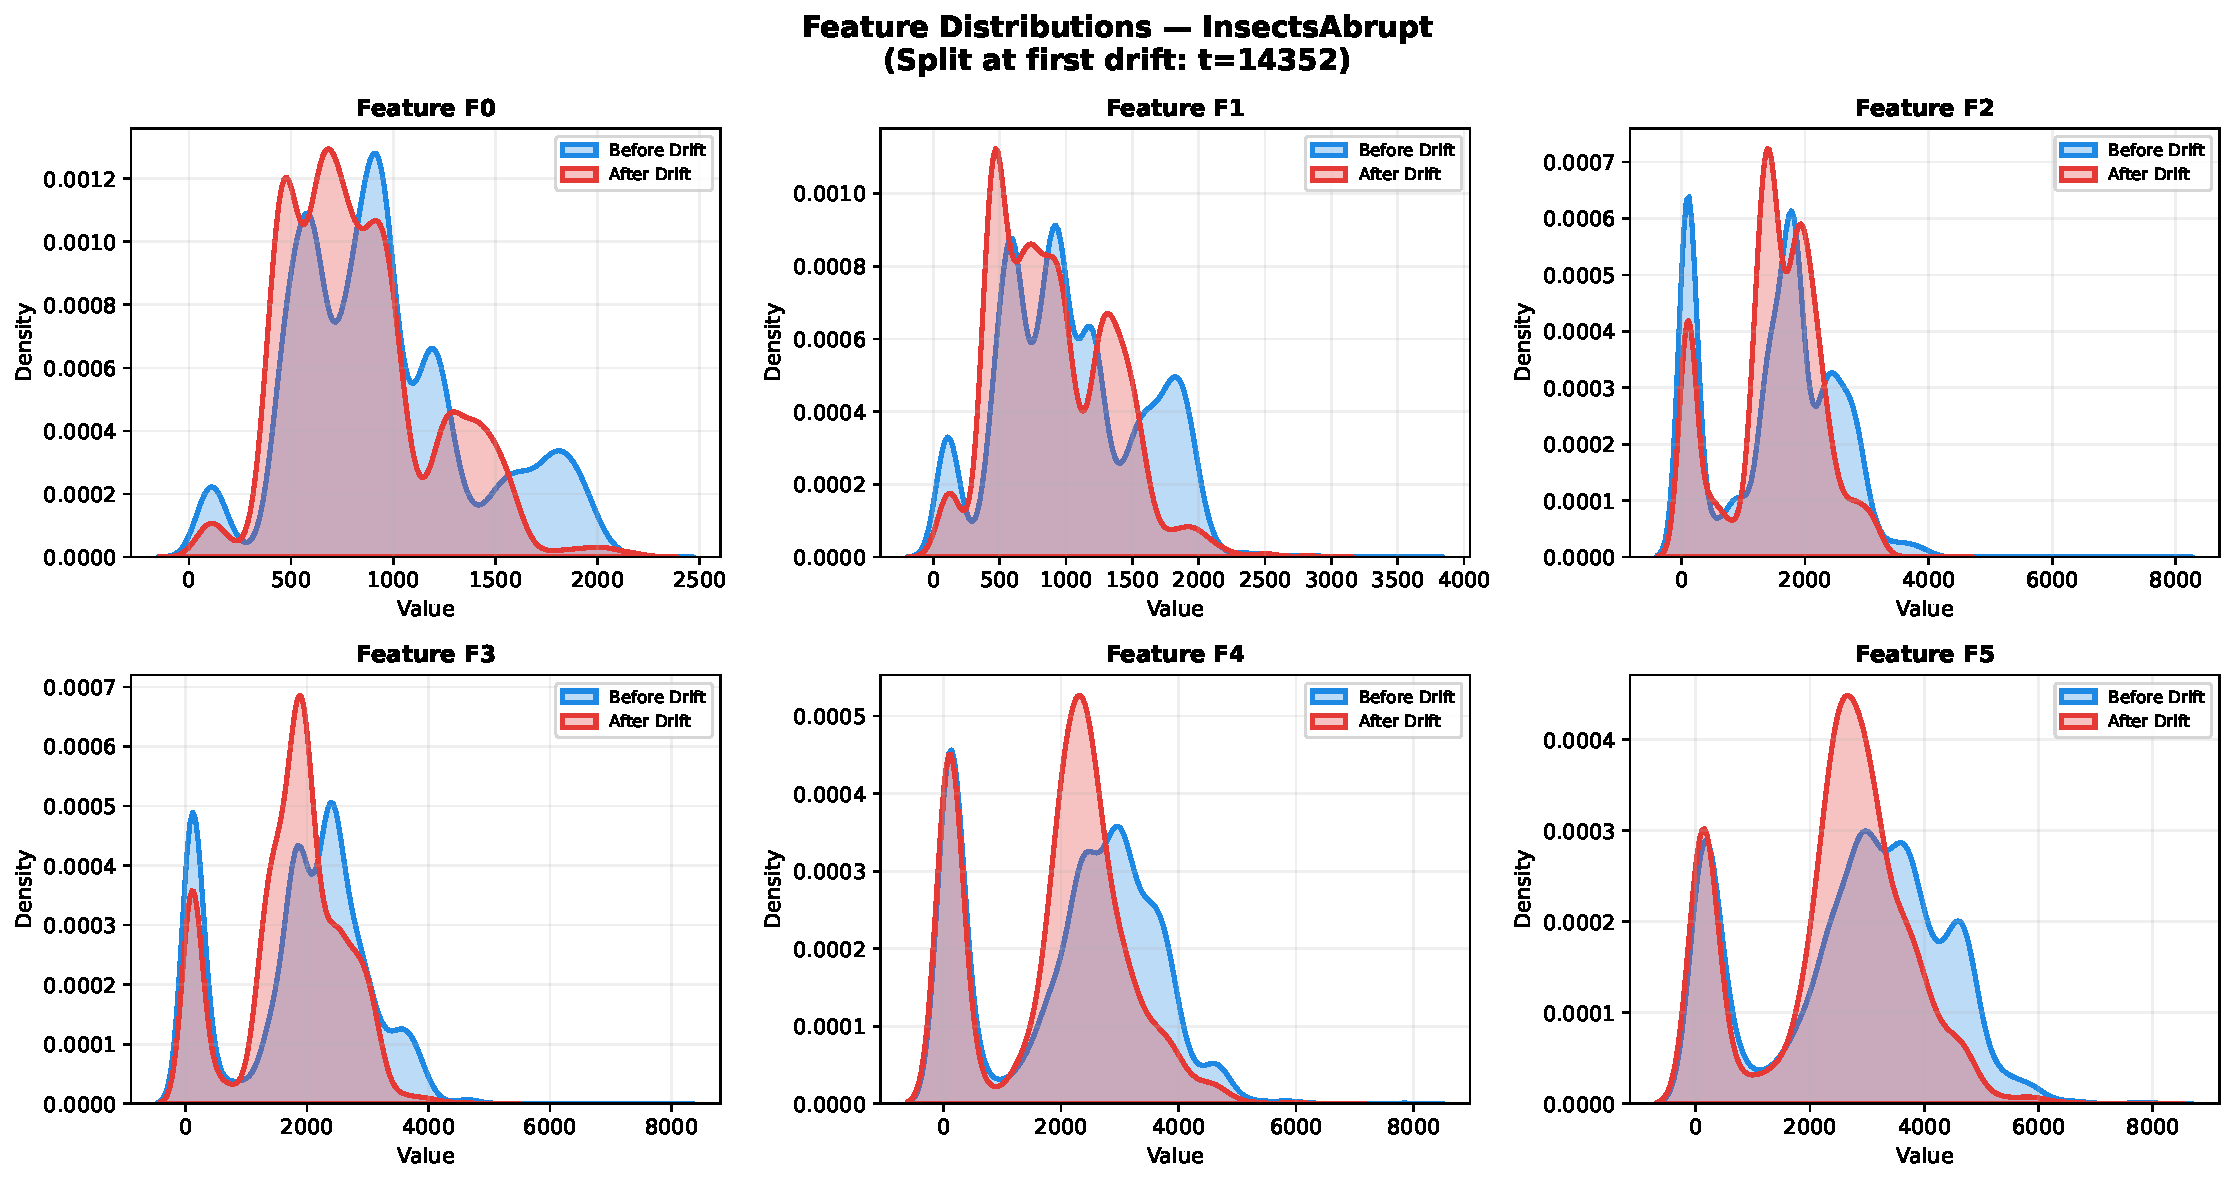
\includegraphics[width=0.86\textwidth,height=0.34\textheight,keepaspectratio]{figures/bell_curves_realworld_insectsabrupt.pdf}
    \caption[Feature distributions of WaveformDrift2 and InsectsAbrupt]{Feature distribution bell curves. Top: WaveformDrift2 (semi-synthetic) showing multi-dimensional distributional shift across 21 features. Bottom: InsectsAbrupt showing abrupt distributional changes across 33 features.}
    \label{fig:bell-curves-realworld}
\end{figure}

\textbf{Key Findings:}
The real-world benchmark reveals important trade-offs among detectors:

\begin{enumerate}
    \item \textbf{EADD's Real-World Performance:} EADD detected drift on three of the four annotated datasets (Table~\ref{tab:exp2-results}) and had a lower mean MTD than D3 on all three: InsectsAbrupt (124 vs.\ 166), InsectsIncrAbrupt (50 vs.\ 126) and InsectsIncrRecur (84 vs.\ 256). The difference is largest on the incremental drift types. D3 had a higher recall on InsectsAbrupt (0.73 vs.\ 0.60) and InsectsIncrRecur (1.00 vs.\ 0.83), and a higher precision on all three. On the nine unannotated datasets (Table~\ref{tab:exp2-nogt}), EADD and D3 produced almost the same total number of detections (474.7 and 471.7), indicating comparable selectivity when both use the same window sizes.

    \item \textbf{Variation across Runs:} Results varied between seeds because D3's cross-validation folds and EADD's reservoir sampling and permutations are random. For example, EADD's MTD on InsectsIncrAbrupt ranged from 33 to 58, and D3's MTD on InsectsIncrRecur from 172 to 324. An earlier single run without fixed seeds, reported in the conference version of this work, gave larger differences in favour of EADD (e.g., 33 vs.\ 272.5 on InsectsIncrAbrupt); the three-seed averages above are more reliable.

    \item \textbf{IBDD's False Alarm Problem:} In the supplementary run, IBDD demonstrated the fastest raw detection times (MTD = 8--88) but at enormous false alarm cost: 726 detections on Electricity, 485 on NOAAWeather and 163 on Powersupply. Over the 11 streams, IBDD raised 2{,}509 detections and OCDD 700, compared with 99 for EADD and 129 for D3.

    \item \textbf{BNDM's Scalability Limitation:} BNDM timed out on all 33-feature datasets (InsectsAbrupt, InsectsGradual, InsectsIncrAbrupt, InsectsIncremental, InsectsReoccurring), making it impractical for high-dimensional real-world data.

    \item \textbf{InsectsGradual Challenge:} InsectsGradual remained one of the hardest datasets: EADD, D3, BNDM, OCDD and UDetect all missed the annotated drift point, while CSDDM, IBDD and SPLL detected it at the cost of more detections on other datasets. EADD raised an alarm 29 samples before the annotated drift point in the run with seed 42; because the matching rule only accepts detections at or after the drift point, this alarm counts as a false alarm.
\end{enumerate}

\section{Experiment 3: Robustness to Stable Data (False Alarm Evaluation)}
\label{sec:exp4}

\textbf{Objective:} Measure false alarm rates on stable data streams that contain no drift.

\textbf{Experimental Design:}
The four stable streams described in Section~\ref{sec:datasets} (Gaussian i.i.d., autocorrelated AR(1), heteroscedastic, and correlated features; $n = 10{,}000$ each) were each generated five times with different seeds. EADD ($N_{ref} = 500$, $N_{cur} = 200$) and D3 ($N_{ref} = 100$, $N_{cur} = 50$) were run on every stream, with D3 at AUC thresholds $\tau \in \{0.6, 0.7, 0.8\}$.

\textbf{Results:}
EADD produced zero false alarms across all four stream types. D3 was particularly vulnerable to autocorrelated data: 87.4 mean false alarms at $\tau{=}0.6$, 54.6 at $\tau{=}0.7$ and 13.8 at $\tau{=}0.8$. At $\tau{=}0.6$, D3 also raised about 10 false alarms on each of the other three streams. Table~\ref{tab:ablation-fa} in Experiment~4 reports the full results.

\textbf{Key Finding:} EADD produced no false alarms, whereas D3 with its small windows raised many false alarms on autocorrelated data at every threshold. D3 used smaller windows than EADD in this experiment, so the comparison does not show whether the difference comes from the window sizes, the classifier, or the permutation test. Experiment~4 separates these effects. The result is consistent with Experiment~2, where D3 used the same window sizes as EADD and both detectors produced almost the same number of detections on the nine unannotated streams.

\section{Experiment 4: Component Ablation}
\label{sec:exp-ablation}

\textbf{Objective:} Determine which of EADD's design choices causes its differences from D3: the classifier, the window sizes, the reference memory, the AUC threshold, or the permutation test.

\textbf{Procedure:}
D3, the ablation variants of Section~\ref{sec:baselines}, and EADD were run on the four synthetic drift streams of Experiment~1 with five seeds (42, 142, 242, 342 and 442), on the four stable streams of Experiment~3 with five runs each, and on the 13 real-world streams of Experiment~2 with three seeds. On the synthetic drift streams, D3 and D3-LightGBM used the window sizes of Experiment~1 ($N_{ref} = 300$, $N_{cur} = 120$). On the stable streams, they used the window sizes of Experiment~3 ($N_{ref} = 100$, $N_{cur} = 50$) at $\tau \in \{0.6, 0.7, 0.8\}$, and EADD's window sizes ($N_{ref} = 500$, $N_{cur} = 200$) at $\tau = 0.7$. On the real-world streams, all variants used EADD's window sizes. D3-LightGBM used the same LightGBM hyperparameters as EADD.

\subsection{Synthetic Streams}

Table~\ref{tab:ablation-drift} reports detection on the synthetic drift streams, and Table~\ref{tab:ablation-fa} reports false alarms on the stable streams.

\begin{table}[!htbp]
\centering
\caption[Experiment 4: ablation on synthetic drift streams]{Experiment 4: Detection on the synthetic drift streams over five seeds. Det.\ = number of seeds in which the drift was detected; MTD = mean time to detection (samples) over the detected seeds; ``--'' = not detected in any seed. Windows are given as $N_{ref}/N_{cur}$.}
\label{tab:ablation-drift}
\small
\setlength{\tabcolsep}{4pt}
\begin{tabular}{l|c|cc|cc|cc|cc}
\hline
 & & \multicolumn{2}{c|}{\textbf{Abrupt}} & \multicolumn{2}{c|}{\textbf{Gradual}} & \multicolumn{2}{c|}{\textbf{Incremental}} & \multicolumn{2}{c}{\textbf{Recurring}} \\
\textbf{Detector} & \textbf{Windows} & Det. & MTD & Det. & MTD & Det. & MTD & Det. & MTD \\
\hline
D3 & 300/120 & 5/5 & 98 & 0/5 & -- & 0/5 & -- & 5/5 & 133 \\
D3-LightGBM & 300/120 & 5/5 & 98 & 0/5 & -- & 0/5 & -- & 5/5 & 117 \\
D3-LightGBM & 500/200 & 5/5 & 210 & 0/5 & -- & 1/5 & 1411 & 5/5 & 175 \\
EADD-NoASPT, fixed ref. & 500/200 & 5/5 & 109 & 5/5 & 549 & 5/5 & 589 & 5/5 & 132 \\
EADD-NoASPT & 500/200 & 5/5 & 139 & 5/5 & 699 & 5/5 & 859 & 5/5 & 149 \\
EADD & 500/200 & 5/5 & 139 & 5/5 & 699 & 5/5 & 859 & 5/5 & 149 \\
\hline
\end{tabular}
\end{table}

All detectors in Table~\ref{tab:ablation-drift} raised no false alarms on the drift streams, with three exceptions: EADD-NoASPT with a fixed reference raised a mean of 1.0 false alarms per stream on gradual drift and 2.0 on incremental drift, and EADD-NoASPT raised 0.2 on incremental drift (one false alarm in five seeds).

\begin{table}[!htbp]
\centering
\caption[Experiment 4: false alarms on stable streams]{Experiment 4: Mean number of false alarms on the stable streams over five runs. Windows are given as $N_{ref}/N_{cur}$.}
\label{tab:ablation-fa}
\begin{tabular}{l|c|c|cccc}
\hline
\textbf{Detector} & \textbf{Windows} & $\boldsymbol{\tau}$ & \textbf{Gaussian} & \textbf{AR(1)} & \textbf{Heterosc.} & \textbf{Correlated} \\
\hline
D3 & 100/50 & 0.6 & 10.4 & 87.4 & 10.4 & 10.0 \\
D3 & 100/50 & 0.7 & 0.0 & 54.6 & 0.0 & 0.0 \\
D3 & 100/50 & 0.8 & 0.0 & 13.8 & 0.0 & 0.0 \\
D3-LightGBM & 100/50 & 0.6 & 12.2 & 83.8 & 11.8 & 10.8 \\
D3-LightGBM & 100/50 & 0.7 & 0.0 & 52.2 & 0.0 & 0.0 \\
D3-LightGBM & 100/50 & 0.8 & 0.0 & 8.6 & 0.0 & 0.0 \\
D3 & 500/200 & 0.7 & 0.0 & 0.0 & 0.0 & 0.0 \\
D3-LightGBM & 500/200 & 0.7 & 0.0 & 0.2 & 0.0 & 0.0 \\
EADD-NoASPT & 500/200 & 0.7 & 0.0 & 0.0 & 0.0 & 0.0 \\
EADD & 500/200 & 0.7 & 0.0 & 0.0 & 0.0 & 0.0 \\
\hline
\end{tabular}
\end{table}

\subsection{Real-World Streams}

Table~\ref{tab:ablation-realworld} reports the ablation on the real-world streams, where all variants used the same window sizes ($N_{ref} = 500$, $N_{cur} = 200$). All variants missed the drift in InsectsGradual.

\begin{table}[!htbp]
\centering
\caption[Experiment 4: ablation on real-world streams]{Experiment 4: Ablation on the real-world streams, averaged over three seeds. Rec.\ = recall; MTD = mean time to detection (samples); the last column is the total number of detections on the nine unannotated streams.}
\label{tab:ablation-realworld}
\small
\setlength{\tabcolsep}{4pt}
\begin{tabular}{l|cc|cc|cc|c}
\hline
 & \multicolumn{2}{c|}{\textbf{InsectsAbrupt}} & \multicolumn{2}{c|}{\textbf{InsectsIncrAbrupt}} & \multicolumn{2}{c|}{\textbf{InsectsIncrRecur}} & \textbf{Unannotated} \\
\textbf{Detector} & Rec. & MTD & Rec. & MTD & Rec. & MTD & \textbf{detections} \\
\hline
D3 & 0.73 & 166 & 1.00 & 126 & 1.00 & 256 & 471.7 \\
D3-LightGBM & 0.80 & 130 & 1.00 & 176 & 0.67 & 197 & 511.7 \\
EADD-NoASPT & 0.60 & 107 & 0.33 & 85 & 1.00 & 108 & 477.1 \\
EADD & 0.60 & 124 & 1.00 & 50 & 0.83 & 84 & 474.7 \\
\hline
\end{tabular}
\end{table}

\subsection{Effect of the AUC Threshold}

Because ASPT runs only when the AUC exceeds $\tau$, its effect depends on the threshold. Table~\ref{tab:ablation-threshold} compares EADD with and without ASPT at $\tau \in \{0.5, 0.6, 0.7\}$ on the synthetic streams. Every variant detected every synthetic drift in all five seeds.

\begin{table}[!htbp]
\centering
\caption[Experiment 4: effect of the AUC threshold on ASPT]{Experiment 4: Effect of the AUC threshold $\tau$ on EADD with and without ASPT (synthetic streams; five seeds or runs). FA = mean false alarms per stable stream; MTD = mean time to detection on the drift streams; the last column gives the mean number of ASPT invocations and rejections per stable stream.}
\label{tab:ablation-threshold}
\small
\setlength{\tabcolsep}{4pt}
\begin{tabular}{c|l|c|ccc|c}
\hline
 & & \textbf{Stable} & \multicolumn{3}{c|}{\textbf{MTD}} & \textbf{ASPT} \\
$\boldsymbol{\tau}$ & \textbf{Variant} & \textbf{FA} & Abrupt & Gradual & Incremental & \textbf{invoked / rejected} \\
\hline
0.5 & EADD-NoASPT & 4.35 & 79 & 229 & 369 & -- \\
0.5 & EADD & 2.10 & 79 & 369 & 559 & 25.6 / 23.5 \\
0.6 & EADD-NoASPT & 0.70 & 99 & 539 & 639 & -- \\
0.6 & EADD & 0.70 & 99 & 539 & 639 & 0.7 / 0.0 \\
0.7 & EADD-NoASPT & 0.00 & 139 & 699 & 859 & -- \\
0.7 & EADD & 0.00 & 139 & 699 & 859 & 0.0 / 0.0 \\
\hline
\end{tabular}
\end{table}

Lowering $\tau$ made detection faster but raised more false alarms. At $\tau = 0.5$, ASPT rejected 92\% of the alarms it tested on the stable streams and halved the false alarms (2.10 vs.\ 4.35 per stream), at the cost of slower detection of gradual and incremental drift (MTD 369 vs.\ 229 and 559 vs.\ 369). At $\tau = 0.6$ and $\tau = 0.7$, ASPT rejected no alarm, so EADD and EADD-NoASPT behaved the same. Even with ASPT, EADD at $\tau = 0.5$ raised 2.10 false alarms per stable stream and 5.2 on the autocorrelated stream, because every monitoring check is a separate test at $\alpha = 0.05$ and autocorrelation violates the exchangeability that the permutation test assumes.

\textbf{Key Findings:}

\begin{enumerate}
    \item \textbf{Classifier:} Replacing logistic regression with LightGBM in D3 changed little. On the synthetic streams, D3-LightGBM detected the same drift types as D3, abrupt and recurring drift, and missed gradual and incremental drift in all five seeds; on stable data it produced false alarm counts similar to D3 (52.2 vs.\ 54.6 on AR(1) at $\tau = 0.7$). On the real-world streams, D3-LightGBM had a higher recall than D3 on InsectsAbrupt (0.80 vs.\ 0.73) but a lower recall on InsectsIncrRecur (0.67 vs.\ 1.00), and it raised more detections on the unannotated streams (511.7 vs.\ 471.7). The LightGBM classifier is therefore not what allows EADD to detect gradual and incremental drift.

    \item \textbf{Window size:} With EADD's window sizes, D3 and D3-LightGBM produced almost no false alarms on the stable streams (0.0 and 0.2 on AR(1)). The false alarms of D3 in Experiment~3 are therefore caused mainly by its small windows, which make the AUC estimate noisy, especially when consecutive samples are correlated. Larger windows alone did not let D3-LightGBM detect gradual drift, and it detected incremental drift in only one of five seeds, 1{,}411 samples after onset.

    \item \textbf{Reference memory:} Every variant with a long-memory reference window detected all four synthetic drift types in all five seeds. D3 compares two adjacent windows that move forward together, so a drift that develops over 1{,}000 to 2{,}000 samples never makes the two windows very different. EADD's reference window instead represents all samples since the last confirmed drift, through reservoir sampling, or keeps the first samples after it (fixed reference), so a slow change accumulates in the comparison. The fixed reference detected gradual and incremental drift sooner (MTD 549 and 589 vs.\ 699 and 859) but raised 1.0 and 2.0 false alarms per stream, while reservoir sampling raised 0.0 and 0.2. On the real-world streams, EADD detected the two incremental INSECTS streams much sooner than D3-LightGBM, which uses the same classifier and window sizes (MTD 50 vs.\ 176 and 84 vs.\ 197).

    \item \textbf{Permutation test and threshold:} ASPT never overturned an alarm at the default threshold $\tau = 0.7$. EADD-NoASPT, which accepts every AUC above $\tau$, raised no false alarms on the stable streams, so the AUC never exceeded $\tau = 0.7$ there and ASPT was never invoked. On the real-world streams, ASPT was invoked at 1{,}548 of 20{,}322 monitoring checks (7.6\%) and confirmed drift every time. The small differences between EADD and EADD-NoASPT in Tables~\ref{tab:ablation-drift} and~\ref{tab:ablation-realworld} come from the random numbers that ASPT draws, which change the later reservoir samples, and not from ASPT rejecting alarms. ASPT changed the decisions only at $\tau = 0.5$, where it halved the false alarms (Table~\ref{tab:ablation-threshold}).

    \item \textbf{Runtime:} On the stable streams, EADD and EADD-NoASPT took about 11.9 seconds per 10{,}000-sample stream, compared with 0.2 to 0.5 seconds for D3 and 0.9 to 1.3 seconds for D3-LightGBM. Processing all 13 real-world streams once took about 27.5 minutes for EADD, 1.7 minutes for D3-LightGBM and 0.5 minutes for D3. Most of EADD's cost comes from training a LightGBM classifier with 5-fold cross-validation every 50 samples.
\end{enumerate}

\section{Statistical Hypothesis Testing}
\label{sec:h1}

\subsection{H1: Detection Coverage and Delay}

\textbf{H1a: Drift Type Coverage}

Table~\ref{tab:h1a-coverage} summarises the drift-type coverage of the eight detectors in Experiment~1.

\begin{table}[!htbp]
\centering
\caption[Drift type coverage summary]{Drift Type Coverage Summary (out of 4 types: Abrupt, Gradual, Incremental, Recurring)}
\label{tab:h1a-coverage}
\begin{tabular}{lccl}
\hline
\textbf{Detector} & \textbf{Types Detected} & \textbf{Coverage} & \textbf{Mean FA per Type} \\
\hline
\textbf{EADD} & \textbf{4/4} & \textbf{100\%} & \textbf{0.00} \\
BNDM & 4/4 & 100\% & 4.75 \\
CSDDM & 4/4 & 100\% & 5.50 \\
IBDD & 4/4 & 100\% & 46.25 \\
OCDD & 4/4 & 100\% & 17.50 \\
D3 & 2/4 & 50\% & 0.00 \\
SPLL & 2/4 & 50\% & 0.00 \\
UDetect & 0/4 & 0\% & -- \\
\hline
\end{tabular}
\end{table}

EADD is the only detector that achieved full drift-type coverage (4/4) with zero false alarms. BNDM, CSDDM, IBDD, and OCDD also achieved 4/4 coverage but with substantially higher false alarm counts (4.75--46.25 per type). D3 and SPLL each cover only 2/4 types (failing on gradual and incremental drift), while UDetect fails on all four types.

To test H1a, the 20 synthetic drift streams of Experiment~4 (four drift types and five seeds) were compared pairwise. EADD detected the drift in 10 streams where D3 missed it (all gradual and incremental streams), and D3 detected none that EADD missed. The exact one-sided sign test gives $p = 0.001$, so H1a is supported.

\textbf{H1b: Detection Delay Comparison}

On the 10 synthetic streams where both detectors detected the drift (abrupt and recurring), D3 was faster than EADD by 28.6 samples on average (98 vs.\ 139 on abrupt drift and 133 vs.\ 149 on recurring drift). The two-sided Wilcoxon signed-rank test gives $p = 0.020$. H1b, that EADD's delay is comparable to D3's where both detect, is therefore not supported on the synthetic streams: D3 detects abrupt and recurring drift sooner, partly because its windows are smaller. On the real-world streams, where both detectors used the same window sizes, EADD had the lower mean MTD on all three detected streams (Table~\ref{tab:exp2-results}).

\subsection{H2: False Alarm Reduction (Mann--Whitney U Test)}

False alarm counts from EADD and D3 over the four stable stream types were compared using one-sided Mann--Whitney U tests (Experiment~3, Section~\ref{sec:exp4}).

\textbf{Result (vs D3 $\tau$=0.6):} $U = 0.0$, exact $p = 0.014$ (normal approximation $p = 0.010$). The difference is statistically significant: EADD produced 0 mean false alarms in total, compared with 118.2 for D3.

\textbf{Result (vs D3 $\tau$=0.7):} $U = 6.0$, exact $p = 0.343$ (normal approximation $p = 0.227$). Not statistically significant at the $\alpha=0.05$ level.

H2 is therefore supported at $\tau = 0.6$ for D3 with its small windows. Experiment~4 shows, however, that D3 with EADD's window sizes also produces no false alarms on these streams, so the difference cannot be attributed to the permutation test.

\section{Component Analysis on Real-World Data}
\label{sec:component-analysis}

The monitoring logs of EADD on the real-world streams of Experiments~2 and~4 (13 streams, three seeds, 20{,}322 monitoring checks) show how each component behaves.

\textbf{AUC Trajectory.} On InsectsAbrupt, the cross-validated AUC before the first drift point ($t = 14{,}352$) averaged 0.45 and ranged from 0.22 to 0.77. After the drift point it rose from 0.36 to 0.46, 0.58 and 0.76 over three consecutive checks, and EADD confirmed the drift at $t = 14{,}499$, 147 samples after onset (seed 42). Values of the AUC below 0.5 are expected under cross-validation when the windows cannot be separated.

\textbf{ASPT Behaviour.} ASPT was invoked at 1{,}548 checks (7.6\%), each time because the AUC exceeded $\tau = 0.7$. It confirmed drift in every invocation and always stopped at $i = 20$ permutations, the earliest stopping point for $\alpha = 0.05$ ($p = 1/21 \approx 0.048$). A fixed-budget test with 199 permutations would have retrained the classifier 199 times at each of these checks, so ASPT saved 90\% of the permutations. ASPT never stopped early to accept the null hypothesis on these streams, because it was never invoked on an AUC below 0.7.

\textbf{Prediction Entropy.} $H_{\text{pred}}$ was about 0.45 to 0.47 on stable segments and fell together with the AUC as drift appeared, for example to 0.39 and 0.30 in the two checks before the first detection on InsectsAbrupt. Across all checks, the Spearman correlation between $H_{\text{pred}}$ and the AUC was $-0.56$. On InsectsGradual, $H_{\text{pred}}$ stayed between 0.44 and 0.47 around the annotated drift point. These logs do not show $H_{\text{pred}}$ declining consistently before the AUC, so its value as an early-warning signal is not established.

\textbf{Component Summary.} The reservoir-sampled reference window gives EADD its broader detection coverage over D3; the LightGBM classifier alone does not (Experiment~4). At the default threshold, ASPT confirmed every alarm that reached it at 10\% of the cost of a fixed-budget permutation test, so its effect on the decisions depends on the threshold. $H_{\text{pred}}$ provides a continuous monitoring signal but moved together with the AUC. The TreeSHAP feature ranking adds diagnostic output without affecting detection decisions.

\chapter{Discussion} \label{chap:discussion}

This chapter interprets the results of Chapter~\ref{chap:results}, answers the research questions, and relates the findings to the studies reviewed in Chapter~\ref{chap:literature}.

\section{Answers to the Research Questions}

\subsection{RQ1: Detection Accuracy}

\textit{Does EADD achieve comparable or better drift detection performance than state-of-the-art unsupervised detectors?}

The experiments give a nuanced answer: EADD is not the \textit{fastest} detector, but it achieves the best \textit{balance} of coverage and false alarm control among the eight detectors tested.

\begin{itemize}
    \item \textbf{Synthetic Data (Experiments 1 and 4):} EADD detected all four drift types (4/4) with zero false alarms, the only detector among the eight to achieve this combination. BNDM, CSDDM, IBDD, and OCDD also detected 4/4 types but with 4.75--46.25 false alarms per type. D3 and SPLL detected only 2/4 types, failing on gradual and incremental drift. Over 20 paired synthetic streams, EADD detected 10 drifts that D3 missed and D3 none that EADD missed (sign test $p = 0.001$, H1a supported). Where both detected the drift, D3 was faster (Wilcoxon $p = 0.020$, H1b not supported).

    \item \textbf{Real-World Data (Experiment 2):} With matched window sizes and three seeds, EADD detected drift on 3 of 4 annotated INSECTS datasets and had a lower mean MTD than D3 on all three (124 vs.\ 166, 50 vs.\ 126, and 84 vs.\ 256 samples), while D3 had a higher recall on two of them. On nine unannotated datasets, EADD and D3 produced almost the same number of detections (474.7 and 471.7).

    \item \textbf{Source of the Coverage:} Experiment~4 shows that EADD's advantage on gradual and incremental drift comes from its long-memory reference window. D3 with a LightGBM classifier still missed these drift types, even with EADD's window sizes, while EADD without its permutation test detected them in all five seeds.
\end{itemize}

Among the eight detectors, EADD was the only one to combine complete synthetic drift-type coverage with zero false alarms, and on the real-world streams it detected incremental drift sooner than D3.

\subsection{RQ2: Robustness}

\textit{Does EADD's permutation test reduce false alarm rates on stable data compared with threshold-based approaches such as D3?}

EADD produced no false alarms on the four stable streams, while D3 with $N_{ref} = 100$ produced up to 87.4 false alarms at $\tau = 0.6$ and 54.6 at $\tau = 0.7$ on the autocorrelated stream (Experiment~3). The difference at $\tau = 0.6$ was statistically significant (H2, exact $p = 0.014$). The ablation in Experiment~4, however, shows that the permutation test is not the cause of this difference:
\begin{itemize}
    \item \textbf{Window size:} D3 with EADD's window sizes produced no false alarms on any stable stream, and D3-LightGBM produced 0.2 on the autocorrelated stream. The false alarms of D3 in Experiment~3 come from its small windows, which give a noisy AUC estimate when consecutive samples are correlated.

    \item \textbf{Permutation test at the default threshold:} With $\tau = 0.7$, ASPT never rejected an alarm. On the stable streams the AUC never exceeded the threshold, and on the real-world streams ASPT confirmed all 1{,}548 alarms it tested.

    \item \textbf{Permutation test at a lower threshold:} With $\tau = 0.5$, ASPT rejected 92\% of the alarms it tested and halved the false alarms on the stable streams (2.10 vs.\ 4.35 per stream), but EADD still raised more false alarms than at $\tau = 0.7$ and detected gradual and incremental drift more slowly than without ASPT.
\end{itemize}

The answer to RQ2 is therefore that EADD raises fewer false alarms than D3 in its benchmark configuration, but that, at the default threshold, the permutation test did not measurably reduce false alarms. The AUC threshold and the window sizes did. ASPT reduces false alarms only when the threshold is close to 0.5, and even then it cannot keep the number of false alarms per stream at the nominal level, because each monitoring check is a separate test.

\section{Relation to Previous Studies}

Several results agree with the studies reviewed in Chapter~\ref{chap:literature}. \citet{Lukats2024} found that the size of the observed samples was one of the most influential hyperparameters of unsupervised drift detectors, and that D3 is sensitive to noise. The ablation confirms both points for discriminative detectors: changing D3's windows from 100/50 to 500/200 samples removed almost all of its false alarms, while changing its classifier did not. \citet{Lukats2024} also questioned whether purging the data windows after a detection, as most detectors do, suits incremental and gradual drift. The results support this concern from the other side: D3, which compares two adjacent sliding windows, missed every slow synthetic drift, while EADD, whose reference window summarises all data since the last detection, detected all of them.

The behaviour of ASPT follows from the theory of the classifier two-sample test \citep{LopezPazOquab2017}. Under the null hypothesis, the AUC of a classifier trained on shuffled labels concentrates near 0.5, with a spread that shrinks as the windows grow. With 700 samples per test, an AUC of 0.7 lies far in the tail of this distribution, so a permutation test confirms almost every alarm that passes the threshold. The sequential stopping rule of \citet{Gandy2009} still reduced the cost of the test by 90\%, as expected when the evidence is clear. The remaining false alarms at $\tau = 0.5$ illustrate a known limitation of repeated significance testing on a stream: a test at level $\alpha$ at every check does not control the error rate over the whole stream, which is the motivation for anytime-valid tests such as E-C2ST \citep{EC2ST2024}.

The feature ranking in EADD follows the domain-classifier approach of \citet{Maggio2021}, and the monitoring of explanation distributions by \citet{Mougan2025} offers an alternative that observes the deployed model instead. Because the accuracy of the ranking was not evaluated in this thesis, the results neither confirm nor contradict the reports that SHAP rankings identify drifted features. Finally, prediction-based monitoring depends on calibrated outputs \citep{Guo2017, Ovadia2019}. In EADD, the prediction entropy of the discriminator moved together with its AUC, so it added little information beyond the AUC in these experiments.

\section{Practical Implementation Considerations}

\subsection{Window Size and Threshold Selection}

The experiments used $N_{ref} = 500$ and $N_{cur} = 200$ for EADD throughout, which proved effective across both synthetic and real-world datasets. However, the optimal window configuration is dataset-dependent:

\begin{table}[!htbp]
\centering
\caption[Guidelines for window size selection]{Guidelines for Window Size Selection Based on Experimental Evidence}
\label{tab:window-guidelines}
\begin{tabular}{p{3cm}p{4cm}p{5cm}}
\hline
\textbf{Factor} & \textbf{Consideration} & \textbf{Recommendation} \\
\hline
Dataset Size & Larger datasets allow larger windows & $N_{ref}$: 1--10\% of total data \\
Expected Drift Type & Abrupt: smaller windows; Gradual: larger windows & Abrupt: 200--500; Gradual: 500--2000 \\
Detection Latency & Smaller windows = faster detection & Trade-off with statistical power \\
Computational Budget & Larger windows = more expensive training & Balance accuracy vs. speed \\
\hline
\end{tabular}
\end{table}

Experiment~4 shows that window size matters more than the classifier for false alarms on autocorrelated data. With $N_{ref} = 100$, D3 raised false alarms at every threshold from 0.6 to 0.8, while with $N_{ref} = 500$ it raised none at $\tau = 0.7$. The reference memory matters for slow drift: a reference window that summarises all data since the last drift detected gradual and incremental drift that two adjacent sliding windows missed. The threshold sets a trade-off between speed and false alarms: lowering $\tau$ from 0.7 to 0.5 halved the detection delay on gradual drift but introduced false alarms, and ASPT is useful only in that low-threshold setting.

\subsection{Proposed MLOps Deployment Architecture}

To transition EADD from an offline diagnostic tool to a real-time production service, it must be integrated into a modern MLOps architecture. We propose a microservices-based deployment utilising standard data engineering frameworks:

\begin{itemize}
    \item \textbf{Data Ingestion Layer (e.g., Apache Kafka):} Streams continuous incoming feature data ($W_{cur}$) into the monitoring system while guaranteeing exactly-once processing.
    \item \textbf{EADD Monitoring Microservice:} An isolated container running the LightGBM discriminative classifier and SHAP explainer. It utilises Reservoir Sampling to maintain the historical baseline ($W_{ref}$) in an in-memory database (e.g., Redis) for rapid access.
    \item \textbf{Orchestration \& Model Registry (e.g., MLflow / Apache Airflow):} When EADD confirms drift, it pushes a drift report containing the AUC, the p-value, $H_{\text{pred}}$ and the feature ranking to the orchestrator. The orchestrator can then trigger the training pipeline to fetch new data, retrain the primary model and log the new artifact in MLflow, or alert the data engineering team to inspect the upstream pipelines of the top-ranked features.
\end{itemize}

This architecture decouples the computational overhead of the discriminator and the permutation test from the primary model's inference latency, allowing EADD to run asynchronously as an independent monitoring service.

\section{Limitations and Threats to Validity}
\label{sec:limitations}

\textbf{Covariate Drift Only:} EADD detects feature drift ($P(X)$ changes) but cannot directly detect pure concept drift ($P(y|X)$ changes with stable $P(X)$). The hierarchical decomposition of \citet{HDPD2024} addresses this gap but requires labelled data.

\textbf{Synthetic Streams:} The synthetic streams have five independent Gaussian features and mean shifts of two standard deviations. Correlated features, smaller shifts and drift in only some features were not studied in the drift streams, so the results may be optimistic for harder drifts.

\textbf{Few Annotated Real-World Drifts:} Only four real-world streams have annotated drift points, with ten annotated drifts in total, and the annotation marks only major transitions. Precision on these streams is therefore uncertain, and the nine unannotated streams can only be compared by their detection counts.

\textbf{Number of Runs:} Experiment~1 used one stream per drift type and Experiment~3 five runs per stream type, and the real-world results varied between seeds (Section~\ref{sec:exp2}). The statistical tests are based on small samples, such as four stream types for H2.

\textbf{Window Sizes in Experiment 3:} In Experiment~3, D3 used smaller windows than EADD. The H2 result therefore reflects the window sizes as well as the detectors themselves, as Experiment~4 shows.

\textbf{Repeated Testing:} EADD tests for drift at every monitoring check without correcting for the number of tests, and the permutation test assumes exchangeable samples, which autocorrelated streams violate. The false alarm rate per stream is therefore not controlled at $\alpha$.

\textbf{Computational Overhead:} EADD took about 11.9 seconds per 10{,}000-sample stable stream, compared with 0.2 to 0.5 seconds for D3, and about 27.5 minutes for one pass over the 13 real-world streams, compared with 0.5 minutes for D3. Each permutation is independent, so the permutation test can be distributed across compute clusters for high-velocity applications.

\textbf{Unevaluated Feature Ranking:} The TreeSHAP feature ranking is reported with each detection but its accuracy is not evaluated in this thesis. SHAP explanations are also correlational rather than causal \citep{CausalDrift2025}, so in production they may direct attention to symptomatic rather than root-cause features.

\textbf{Difference from the Conference Paper:} The conference version of this work reported a single unseeded real-world run, the Drift Severity Index, and an evaluation of the feature ranking on three synthetic scenarios. This thesis replaces the real-world results with three-seed averages and leaves out the severity index and the ranking evaluation, so some numbers differ between the two documents.

\textbf{Adversarial Vulnerability:} \citet{AdvAttackDrift2024} demonstrated that discriminative drift detectors can be evaded by adversarial data streams. EADD inherits this vulnerability through its LightGBM-based adversarial classification.

\section{Chapter Summary}

EADD was the only detector to achieve 4/4 synthetic drift-type coverage with zero false alarms, and it detected the slow synthetic drifts that D3 missed (RQ1, H1a supported); where both detected the drift, D3 was faster (H1b not supported). On the real-world streams with matched windows, EADD detected incremental drift sooner than D3, and both raised a similar number of detections. EADD produced no false alarms on the stable streams, while D3 with small windows produced up to 87.4 (RQ2, H2 supported at $\tau = 0.6$). The ablation showed that EADD's coverage of slow drift comes from its reservoir-sampled reference window, that D3's false alarms come from its small windows, that replacing D3's logistic regression with LightGBM changes little, and that ASPT changes the decisions only when the AUC threshold is lowered to 0.5. The remaining detection limitation is InsectsGradual, where EADD (along with D3, BNDM, OCDD, and UDetect) missed the annotated drift point.

\addtocontents{toc}{\protect\newpage}

\chapter{Conclusion and Recommendations} \label{chap:conclusion}

\section{Summary of Findings}

This thesis addressed three gaps in D3's operational utility: the lack of a formal significance test, a reference window that moves with the current window, and the absence of any feature-level output. D3 \citep{Gozuacik2019} demonstrated that discriminative classification can detect distribution changes, and recent work \citep{TRIPODD2024, HDPD2024, EC2ST2024} advanced individual aspects of drift detection, but these components had not been combined and evaluated together in an unsupervised streaming detector.

We proposed \textbf{Enhanced Adversarial Drift Detection (EADD)} and made the following contributions:

\begin{enumerate}
    \item An integrated framework that combines a LightGBM classifier two-sample test \citep{LopezPazOquab2017, Ke2017}, a reservoir-sampled reference window \citep{Vitter1985}, prediction entropy monitoring ($H_{\text{pred}}$) and an adaptive sequential permutation test, and that ranks the features behind each confirmed drift with TreeSHAP \citep{Lundberg2017}.
    \item An adaptive sequential permutation test (ASPT) that applies sequential Monte Carlo stopping \citep{Gandy2009} to the classifier two-sample test. ASPT confirmed a clear drift after 20 of 199 permutations, a 90\% saving over a fixed-budget test.
    \item An experimental evaluation against seven unsupervised detectors on synthetic and real-world streams, including an ablation with a LightGBM version of D3 that separates the effects of the classifier, the window sizes, the reference memory, the threshold and the permutation test.
\end{enumerate}

The experimental evaluation (Chapter~\ref{chap:results}) produced the following key findings:
\begin{itemize}
    \item \textbf{Experiment 1:} EADD detected all four synthetic drift types (4/4) with zero false alarms, the only detector to achieve this combination. BNDM, CSDDM, IBDD, and OCDD achieved 4/4 coverage but with substantially higher false alarm counts.
    \item \textbf{Experiment 2:} With matched window sizes and three seeds, EADD detected drift on 3 of 4 annotated INSECTS datasets and had a lower mean MTD than D3 on all three (124 vs.\ 166, 50 vs.\ 126, and 84 vs.\ 256 samples), while D3 had a higher recall on two of them. On nine unannotated datasets, both detectors raised a similar number of detections (474.7 and 471.7).
    \item \textbf{Experiment 3:} EADD produced no false alarms on 4 stable stream types, compared with D3's 87.4 mean false alarms on autocorrelated data at $\tau=0.6$ with $N_{ref} = 100$.
    \item \textbf{Experiment 4:} D3 with a LightGBM classifier behaved like the original D3. With EADD's window sizes, D3 raised almost no false alarms. EADD's coverage of slow drift came from its reservoir-sampled reference window. ASPT changed the decisions only at $\tau = 0.5$, where it halved the false alarms.
\end{itemize}

Statistical testing supported H1a (sign test $p = 0.001$) and H2 at $\tau = 0.6$ (exact Mann--Whitney $p = 0.014$), but not H1b: D3 detected abrupt and recurring drift sooner on the synthetic streams. The ablation showed that the H2 difference is explained by D3's smaller windows rather than by the permutation test.

\section{Limitations}

The main limitations of this study, discussed in Section~\ref{sec:limitations}, are the following. EADD detects only covariate drift. The synthetic streams have independent features and large mean shifts, and only four real-world streams have annotated drift points. Several analyses rely on few runs or stream types. EADD tests at every check without controlling the error rate over a whole stream, and its runtime is 25 to 55 times that of D3. Finally, the TreeSHAP feature ranking was not evaluated.

\section{Recommendations for Application}

The results lead to the following recommendations for practitioners who deploy discriminative drift detectors:

\textbf{Check the Windows First:} For discriminative detectors, the design of the windows matters more than the choice of classifier. A reference window that summarises all data since the last drift detects slow drift that adjacent sliding windows miss, and windows that are too small cause false alarms on autocorrelated data. Window sizes and reference memory should be checked before the classifier or the threshold is changed.

\textbf{Choose the Threshold Deliberately:} With windows of 500 and 200 samples, an AUC threshold of 0.7 gave no false alarms on the stable streams, and a permutation test added nothing at that threshold. A lower threshold detects drift sooner but needs a significance test, such as ASPT, to limit false alarms, and even then some false alarms remain on autocorrelated data.

\textbf{Use ASPT to Make Significance Testing Affordable:} When a permutation test is used, the adaptive sequential stopping rule reduces its cost by about 90\% for clear decisions, making permutation-based calibration practical for moderate-frequency monitoring.

\textbf{Budget for Computation:} EADD's LightGBM classifier with 5-fold cross-validation every 50 samples made it 25 to 55 times slower than D3 in our experiments. Monitoring less often, training fewer trees or running the monitor asynchronously from the primary model can reduce this cost.

\textbf{Treat the Feature Ranking as a Lead:} The TreeSHAP ranking points to the features that separate the two windows, which can direct engineers to upstream data sources before a full retraining. Because its accuracy has not been evaluated and SHAP is correlational \citep{CausalDrift2025}, it should be treated as a lead for investigation rather than as a diagnosis. In regulated sectors, where ``black box'' model adaptations may violate transparency requirements \citep{GoodmanFlaxman2017}, the ranking can also document which features changed before each drift-triggered update.

\section{Suggestions for Future Research}

Based on the experimental findings and the rapidly evolving literature, future research should pursue the following directions:

\begin{enumerate}
    \item \textbf{Evaluating the Feature Ranking:} Measuring how accurately the TreeSHAP ranking identifies drifting features on streams with correlated and interacting features, and on real-world streams with documented causes of drift.

    \item \textbf{Anytime-Valid Testing:} Replacing the per-check permutation p-value with e-values \citep{EC2ST2024} would control the false alarm rate over a whole stream rather than at each check, which the low-threshold results show is needed.

    \item \textbf{Harder Synthetic Drifts and More Annotated Streams:} Evaluating the detectors on correlated features, smaller shifts and drifts in subsets of features, and on more real-world streams with annotated drift points.

    \item \textbf{Prediction Entropy as an Early Warning:} Testing whether $H_{\text{pred}}$, alone or combined with the AUC trend, gives warnings earlier than the AUC threshold, with a quantitative evaluation of its lead time and false warnings.

    \item \textbf{Causal Drift Attribution:} Extending EADD's correlational SHAP explanations toward causal drift attribution \citep{CausalDrift2025} would help remediation target root causes rather than correlated symptoms.

    \item \textbf{Covariate and Concept Drift Decomposition:} Integrating the hierarchical decomposition framework of \citet{HDPD2024} to separate $P(X)$ shifts from $P(y|X)$ shifts when delayed labels become available.

    \item \textbf{Adversarial Robustness:} Developing defences against adversarial drift evasion attacks \citep{AdvAttackDrift2024}, potentially through ensemble diversification or randomised smoothing of the discriminative classifier.

    \item \textbf{Deep Learning Extension:} Adapting EADD for unstructured data (images, text) using deep learning classifiers and embedding-space attribution, building on DriftLens \citep{DriftLens2024}.
\end{enumerate}

\section{Concluding Remarks}

This thesis proposed EADD, an integrated framework that combines established methods: the classifier two-sample test \citep{LopezPazOquab2017}, reservoir sampling \citep{Vitter1985}, sequential Monte Carlo testing \citep{Gandy2009} and TreeSHAP \citep{Lundberg2017, LundbergInteraction2020}. In a single unsupervised streaming pipeline, these components report whether the discriminator can separate recent data from the reference data, whether the separation is statistically significant, and which features drive it. EADD was the only detector in the evaluation to achieve complete synthetic drift-type coverage (4/4) with zero false alarms, and on the real-world streams it detected incremental drift sooner than D3. The ablation showed that much of this behaviour comes from the design of the reference window rather than from the classifier or the permutation test, a result that applies to discriminative drift detectors in general.
